\documentclass[12pt,a4paper]{report}

\usepackage{iftex}
\ifPDFTeX
  \usepackage[T1]{fontenc}
  \usepackage[utf8]{inputenc}
  \usepackage{lmodern}
\else
  \usepackage{fontspec}
  \setmainfont[
    Path=/usr/local/texlive/2026/texmf-dist/fonts/opentype/public/lm/,
    UprightFont={lmroman10-regular.otf},
    BoldFont={lmroman10-bold.otf},
    ItalicFont={lmroman10-italic.otf},
    BoldItalicFont={lmroman10-bolditalic.otf}
  ]{Latin Modern Roman}
  \newfontfamily\arabicfont[
    Path=/System/Library/Fonts/Supplemental/,
    UprightFont={Arial Unicode.ttf}
  ]{Arial Unicode}
\fi

\usepackage[a4paper,left=30mm,right=25mm,top=25mm,bottom=25mm]{geometry}
\usepackage{amsmath,amssymb}
\usepackage{array}
\usepackage{booktabs}
\usepackage{caption}
\usepackage{float}
\usepackage{graphicx}
\usepackage{longtable}
\usepackage{microtype}
\usepackage{placeins}
\usepackage{tabularx}
\usepackage{xcolor}
\usepackage[hidelinks]{hyperref}
\usepackage{pdfpages}
\usepackage{cite}

\graphicspath{{assets/}{../eda/figures/}{../modeling/figures/}{../dashboard/screenshots/}}
\setcounter{tocdepth}{2}

\newcolumntype{Y}{>{\raggedright\arraybackslash}X}
\newcolumntype{L}[1]{>{\raggedright\arraybackslash}p{#1}}
\newcommand{\thesistitle}{Explainable AI for Non-Recurrent Traffic Incident Risk Prediction in Dubai}
\newcommand{\studentname}{Sparsh Aggarwal}
\newcommand{\studentid}{2022A7TS0279U}
\newcommand{\studentdiscipline}{Computer Science}
\newcommand{\supervisor}{Dr.\ Sujala D.\ Shetty}
\newcommand{\supervisordesignation}{Professor, Department of Computer Science}
\newcommand{\supervisorsecondarydesignation}{Associate Dean, Practice School and Industry Engagement}
\newcommand{\director}{Dr.\ Souri Banerjee}
\newcommand{\outgoingassociatedean}{Dr.\ A.\ Somasundaram}
\newcommand{\incomingassociatedean}{Dr.\ Tamizharasan Periyasamy}
\newcommand{\incominghod}{Dr.\ Pranav M.\ Pawar}
\newcommand{\publicrepo}{\url{https://github.com/sparshagg/dubai-traffic-incident-risk-xai}}
\renewcommand{\bibname}{References}

\begin{document}

\begin{titlepage}
    \centering
    \vspace*{1cm}
    {\large THESIS REPORT}\\[0.5cm]
    {\large ON}\\[1cm]
    {\Large \textbf{\MakeUppercase{\thesistitle}}}\\[1cm]
    {\large Submitted in partial fulfillment of the requirements for}\\[0.2cm]
    {\large BITS F423T THESIS}\\[0.8cm]
    {\large BY}\\[0.6cm]
    {\large \textbf{\studentname}}\\[0.2cm]
    {\large \textbf{ID NO \studentid}}\\[1.2cm]
    {\large Under the supervision of}\\[0.4cm]
    {\large \textbf{\supervisor}}\\[0.1cm]
    {\large \supervisordesignation}\\[0.1cm]
    {\large \supervisorsecondarydesignation}\\[1cm]
    \vfill
    \IfFileExists{assets/university_logo.png}{
\includegraphics[width=0.24\textwidth]{assets/university_logo.png}\\[0.6cm]}{}
    {\large ACADEMIC RESEARCH DIVISION}\\[0.25cm]
    {\large BIRLA INSTITUTE OF TECHNOLOGY AND SCIENCE, PILANI}\\[0.2cm]
    {\large DUBAI CAMPUS, DUBAI, U.A.E.}\\[0.7cm]
    {\large June 2026 - July 2026}
\end{titlepage}

\pagenumbering{roman}

\newpage
\thispagestyle{plain}
\begin{center}
    \large \textbf{Summer Term, Academic Year 2025-26}\\
    \textbf{BITS Pilani, Dubai Campus}\\
    \textbf{Dubai International Academic City, Dubai, U.A.E.}
\end{center}
\vspace{0.8cm}
\begin{tabular}{@{}ll}
    \textbf{Course Title} & : Thesis \\
    \textbf{Course Number} & : BITS F423T \\
    \textbf{Report Type} & : Final thesis report \\
    \textbf{Project Repository} & : \publicrepo \\
    \textbf{Date of Submission} & : 31 July 2026 \\
\end{tabular}
\vspace{1cm}
\begin{center}
    \textbf{Title of the Project}\\[0.2cm]
    \Large \textbf{\thesistitle}
\end{center}
\vspace{1.2cm}
\begin{tabularx}{\textwidth}{@{}L{0.32\textwidth}Y@{}}
    \textbf{Student ID Number} & : \studentid \\
    \textbf{Student Name} & : \studentname \\
    \textbf{Student Discipline} & : \studentdiscipline \\
    \\
    \textbf{Supervisor Name} & : \supervisor \\
    \textbf{Supervisor Designation} & : \supervisordesignation; \supervisorsecondarydesignation \\
\end{tabularx}

\vfill
\noindent
\begin{tabular}{p{0.45\textwidth} p{0.45\textwidth}}
    \rule{4cm}{0.4pt} & \rule{4cm}{0.4pt} \\
    \small \textbf{Student Signature} & \small \textbf{Supervisor Signature}
\end{tabular}

\chapter*{Acknowledgements}
\addcontentsline{toc}{chapter}{Acknowledgements}
I thank \director, Director of BITS Pilani Dubai Campus, for providing the academic environment and institutional support needed to undertake this thesis.

I thank \outgoingassociatedean, outgoing Associate Dean, Academic Undergraduate Studies Division, BITS Pilani Dubai Campus, for the academic coordination and guidance connected with the thesis course. I also thank \incomingassociatedean, Associate Dean, Academic Undergraduate Studies Division, for continuing the academic coordination of the thesis process.

I am grateful to \supervisor, my thesis supervisor, for guiding the direction of this work and for helping me keep the topic practical, data-driven, and research focused.

I acknowledge Dr.\ Sujala D.\ Shetty's role as outgoing Head of Department (Computer Science), and I also acknowledge \incominghod, incoming Head of Department (Computer Science), for the continued academic leadership of the department.

I also thank the faculty and staff members who supported access to academic resources and helped with thesis-related requirements during the summer term.

\vspace{1cm}
\noindent \textbf{\studentname}\\
\textbf{\studentid}

\chapter*{Certificate}
\addcontentsline{toc}{chapter}{Certificate}
This is to certify that the thesis entitled, \textit{\thesistitle}, has been submitted by \studentname, ID No. \studentid. The work has been carried out under my supervision in partial fulfillment of the requirements for BITS F423T Thesis.

\vspace{2cm}
\noindent Date:\hfill Signature of the Supervisor

\vspace{1.2cm}
\noindent \hfill \supervisor

\chapter*{List of symbols and abbreviations}
\addcontentsline{toc}{chapter}{List of symbols and abbreviations}
\begin{longtable}{L{0.24\textwidth}L{0.68\textwidth}}
API & Application programming interface. \\
ECE & Expected calibration error. \\
H3 & Hexagonal hierarchical geospatial index system. \\
LIME & Local interpretable model-agnostic explanations. \\
ML & Machine learning. \\
MCE & Maximum calibration error. \\
PR-AUC & Area under the precision-recall curve. \\
ROC-AUC & Area under the receiver operating characteristic curve. \\
SHAP & Shapley additive explanations. \\
XGBoost & Extreme Gradient Boosting. \\
XAI & Explainable artificial intelligence. \\
\end{longtable}

\chapter*{Thesis abstract}
\addcontentsline{toc}{chapter}{Thesis abstract}
This thesis develops an explainable machine-learning framework for non-recurrent traffic incident risk prediction in Dubai. The work uses an open Dubai Police incident dataset from Dubai's Data and Statistics portal. The frozen local snapshot contains 720,155 incident-level records from 13 August 2018 to 1 June 2026. The raw records were audited, translated from Arabic category labels, checked for coordinate-order errors, and converted into H3 grid cells and 3-hour time windows.

The prediction task is defined as a binary grid-time problem: for each inside-Dubai H3 cell and each 3-hour window, the model predicts whether at least one incident will occur. A chronological split is used so that later windows are not used during training. The stronger evaluation uses a full inside-Dubai grid with 1,305 cells, 4,463,100 test candidate cell/windows, and 108,224 positive test cell/windows. Historical risk, Logistic Regression, Random Forest, and XGBoost models were compared. The final selected model is the default XGBoost classifier with same-cell lag features, historical risk priors, and ring-1 neighboring-cell lag features.

Neighboring-cell lag features improve full-grid PR-AUC from 0.0967 to 0.0992 and F1-score from 0.1615 to 0.1645 compared with the same XGBoost setup without neighbor features. The selected model captures 10,416 incidents in the top-20 ranked cells per test window. A 70/30 hard-negative training strategy and a tuned XGBoost configuration were tested but were not promoted because they reduced the untouched full-grid test result. Sigmoid calibration was selected for dashboard display because it reduced Brier score from 0.2127 to 0.0227 while preserving ranking metrics. SHAP is used as the main explanation method, and LIME is used as a selected local comparison. The final dashboard demonstrates the model through a rolling replay with an English dashboard map, ranked risk zones, and SHAP reasons for selected zones.

\tableofcontents
\listoffigures
\listoftables
\newpage

\pagenumbering{arabic}

\chapter{Introduction}

Dubai has a dense and heavily used road network that supports commuting, freight movement, tourism, airport access, and everyday city travel. A traffic incident in such a network can affect more than the vehicles directly involved. A crash, vehicle breakdown, obstruction, roadwork report, or stalled vehicle can reduce road capacity, create a local safety risk, and produce congestion that is different from the regular morning or evening peak pattern. These events are commonly treated as non-recurrent incidents because they are irregular disruptions rather than routine demand.

This thesis studies whether historical incident records can be converted into an explainable machine-learning framework for Dubai. The work is deliberately narrower than citywide traffic optimization. It does not attempt to control traffic signals, simulate vehicle flow, or claim live deployment. The aim is to predict which small areas and 3-hour periods are more likely to contain reported incidents, evaluate that prediction under a chronological design, and explain the model's high-risk outputs in a form that a traffic analyst or examiner can inspect.

The project began with the mid-semester pipeline: data audit, Arabic category mapping, coordinate correction, exploratory analysis, H3 grid construction, and initial baseline models. The final report keeps that pipeline and extends it with inside-Dubai full-grid evaluation, historical-risk leakage checks, H3/time-window sensitivity checks, neighboring-cell features, hard-negative and tuning experiments, probability calibration, SHAP/LIME explanations, and a rolling-replay dashboard. The final contribution is therefore an end-to-end research prototype, from raw incident records to model explanation and visual inspection.

\section{Problem statement}

The source dataset provides incident-level records with occurrence time, Arabic incident category, and geographic coordinates. These fields are useful, but they are not a supervised-learning table by themselves. A supervised model needs examples of both incident and non-incident conditions. It also needs a spatial unit, a time unit, features that are available before the prediction window, and an evaluation design that resembles later use.

The problem addressed in this thesis is:

\begin{quote}
How can Dubai Police incident records be transformed into an explainable grid-time machine-learning framework for predicting non-recurrent traffic incident risk in Dubai?
\end{quote}

The framework must answer three practical questions:

\begin{enumerate}
    \item \textbf{Where} are incident-risk zones likely to appear?
    \item \textbf{When} are those zones likely to be active?
    \item \textbf{Why} does the trained model assign high risk to a selected zone and time window?
\end{enumerate}

The word ``risk'' is used in a model-based sense. It means the model's estimated likelihood that at least one incident will be reported in a specific grid cell and time window. It does not mean that the model has identified the physical cause of an incident. The explanation methods used later in the thesis describe how the model uses the available features, not why a crash or breakdown happened in the real world.

\section{Why grid-time prediction is needed}

The raw incident file is a point dataset. Each record describes one reported incident with a time, category, and coordinate. Point records are useful for mapping and counting incidents, but they are not enough for prediction. A model must also see examples where no incident occurred. For that reason, the thesis converts the point records into grid-time rows. Each row represents one H3 cell and one 3-hour window. If at least one incident occurs in the cell during that window, the row is positive. If no incident occurs, the row is negative.

This formulation is important for two reasons. First, it makes the prediction problem explicit and reproducible. Different researchers can rebuild the same H3 cells and time windows from the same cleaned data. Second, it matches the dashboard goal. A traffic analyst does not need a list of every past incident point; the analyst needs to know which zones and time blocks the model ranks as higher risk and why those zones were ranked that way.

\section{Research objectives}

The thesis has six objectives:

\begin{enumerate}
    \item audit and clean the Dubai Police traffic incident dataset, including Arabic category translation, severity parsing, and coordinate validation;
    \item define a reproducible H3 grid and 3-hour time-window formulation for Dubai incident-risk prediction;
    \item construct binary incident-occurrence labels and leakage-safe temporal, historical-risk, same-cell lag, and neighboring-cell features;
    \item compare baseline and machine-learning models under chronological train, validation, and test splits;
    \item explain the selected model using SHAP and compare selected local cases with LIME;
    \item implement a dashboard that presents ranked risk zones, known replay outcomes, and local explanation reasons on an English dashboard map.
\end{enumerate}

These objectives are ordered to match the actual research workflow. The data audit and grid construction come first because the model depends on them. Model comparison comes after the supervised table is built. Explainability and dashboard work are placed at the end because they must explain the final selected model, not an earlier temporary model.

\section{Research questions}

The work is guided by the following questions:

\begin{enumerate}
    \item Is the open Dubai Police incident dataset usable for grid-time incident-risk modeling after cleaning, translation, and coordinate correction?
    \item Does a machine-learning model improve over a historical cell/time risk baseline when evaluated on the full inside-Dubai grid?
    \item Does nearby H3-cell activity add useful signal beyond same-cell history?
    \item Are the model outputs stable under sensitivity checks for H3 resolution and time-window size?
    \item Can SHAP and LIME explain the selected model's high-risk and error cases in a clear way?
    \item Can the selected model be presented through a dashboard without overstating it as a live traffic-management system?
\end{enumerate}

\section{Main contribution}

The main contribution is a complete, reproducible pipeline for Dubai grid-time incident-risk prediction. The pipeline starts with raw incident records and ends with an explainable dashboard demonstration. It includes data cleaning, translation mapping, coordinate normalization, H3 grid construction, binary target construction, chronological evaluation, full-grid ranking metrics, feature-ablation checks, H3/time-window sensitivity checks, calibration, and SHAP/LIME explanation.

The final selected model is a default XGBoost classifier using H3 resolution 8, 3-hour windows, inside-Dubai cells, same-cell lag features, historical-risk priors, and ring-1 neighboring-cell lag features. The dashboard presents the model through rolling replay. This means the model is shown on the latest fully observed days in the dataset, using the same recent-lag features that would be available immediately before each 3-hour prediction window.

The thesis also contributes a careful evaluation story. The first sampled-negative models show that the end-to-end supervised-learning pipeline works. The stronger result is the inside-Dubai full-grid evaluation, where every inside-Dubai H3 cell is scored for every validation and test window. This distinction prevents the report from overstating sampled-negative metrics as operational performance.

\section{Scope and limitations}

The thesis uses a frozen historical dataset snapshot ending on 1 June 2026. It does not claim live deployment, adaptive traffic signal control, route guidance, or end-to-end traffic management. Forecasts after the data cutoff require updated incident records because the selected model uses recent 3-hour, 24-hour, 7-day, and neighboring-cell lag features.

The work predicts incident occurrence, not incident duration. Duration prediction would require a reliable clearance or resolution timestamp. The available columns include occurrence time and load timestamp, but load timestamp is metadata and is not used as incident clearance time. Weather, road-speed limits, school calendars, public-event data, and detailed road-network attributes are also outside the final model because they were not needed to complete the core incident-only framework.

The result should be read as a reproducible and interpretable baseline. It shows that open Dubai incident records can support grid-time risk modeling after careful preparation. It does not claim that incidents can be perfectly predicted, that high-risk zones are caused by the top SHAP features, or that the dashboard is ready for operational deployment.

Dubai road-safety work motivates the local problem \cite{aldah2010dubai,abdelfatah2015dubai}. Recent Dubai hotspot analysis also supports the value of Dubai Police incident records for spatial and temporal traffic-safety analysis \cite{alsaleh2026dubaihotspots}. This thesis extends that direction from descriptive hotspot analysis to explainable grid-time prediction.

\chapter{Literature review}

This chapter reviews the work most relevant to the thesis: Dubai and UAE road-safety studies, grid-based traffic-risk prediction, non-recurrent incident modeling, explainable AI, and imbalanced evaluation. The purpose is to identify the research gap and justify the methodology used in this report.

The review is used in two ways. The main chapter gives a short synthesis of the papers that shape the thesis design. Appendix A keeps the full reviewed literature matrix so that the broader source base remains visible without making this chapter a catalogue of papers. This structure follows the submitted mid-semester report, but the final report links each literature theme more directly to the implemented method.

\section{Dubai and UAE road-safety context}

Al Dah's Dubai crash thesis established that Dubai road-safety analysis needs local evidence rather than direct transfer of assumptions from other countries \cite{aldah2010dubai}. Abdelfatah et al. studied Dubai accident trends and causes using aggregate accident statistics \cite{abdelfatah2015dubai}. These studies are important because they define the local road-safety context, but they do not build fine-grained prediction models over small spatial units and short time windows.

Abuzaid et al. show that UAE traffic-safety questions can be studied with AI methods \cite{abuzaid2024uae}. Their work is broader than this thesis and is not based on Dubai incident-level grid-time prediction. Alsaleh et al. are closer to this thesis because they use Dubai Police traffic records to study temporal patterns and severity-weighted hotspots \cite{alsaleh2026dubaihotspots}. Their work supports the use of Dubai Police records for spatial analysis, but it remains descriptive. This thesis uses a similar local data source and moves toward predictive modeling and model explanation.

The Dubai and UAE studies define the local need but leave a clear modeling gap. They show that road-safety outcomes in Dubai should be studied with local data, and they show that Dubai Police records can support temporal and spatial analysis. They do not answer whether incident points can be converted into a supervised grid-time table, whether a machine-learning model improves over historical hotspot risk, or whether the model's high-risk outputs can be explained for a selected zone.

\section{Spatiotemporal traffic-risk prediction}

Traffic accident prediction has moved from aggregate trend analysis toward spatiotemporal machine learning. Behboudi et al. review this shift across accident occurrence, severity, frequency, and duration tasks \cite{behboudi2024review}. Ren et al. model citywide accident risk from historical accident patterns \cite{ren2017citywide}. Zhou et al. introduce RiskOracle for fine-grained accident-risk forecasting and highlight sparsity as a central problem in citywide prediction \cite{zhou2020riskoracle}. Chen et al. revisit urban accident-risk prediction and show that regionality, proximity, similarity, and sparsity affect model performance \cite{chen2024urbanrisk}. Other advanced methods, including hierarchical transfer models and transformer-based contextual models, show the same research direction but require richer inputs and heavier architectures than the current thesis uses \cite{an2022hintnet,saleh2022contextualvit}.

These studies support the main structure of this thesis: risk is modeled as a spatial and temporal outcome, not just as a citywide count. They also show why evaluation must consider rare positives. Most grid/time combinations have no incident, so a model can look accurate while failing to rank the genuinely risky locations.

This thesis follows the same broad idea but keeps the data requirements lower. Several advanced spatiotemporal models depend on traffic-flow streams, weather records, road-network graphs, points of interest, or remote-sensing features. Those inputs can improve prediction, but they also make the first Dubai incident-only thesis harder to reproduce from open data. The implemented framework therefore starts with incident history and calendar features, then adds neighboring-cell history as a lightweight spatial signal.

\section{Grid-based and road-level modeling}

Kashifi et al. provide direct support for grid-based crash prediction \cite{kashifi2022grid}. Their work shows that crash records can be aggregated into spatial cells and predicted over time. H3 is used in this thesis for the same practical reason: the Dubai dataset has coordinates, but it does not provide a complete verified road graph, traffic-flow stream, or road-segment attribute table.

Road-level graph models such as Gao et al. and Kim et al. are relevant but require richer spatial structure \cite{gao2023uncertainty,kim2024sstgcn}. Weather-aware crash forecasting and severe-accident studies also show that external covariates can improve risk modeling when reliable weather, traffic-flow, and road-attribute sources are available \cite{ogungbire2026weather,khulbe2019severe}. These studies are useful future-work references because road-network topology and external context can represent mechanisms that grid cells cannot capture directly. For this thesis, H3 gives a simpler and reproducible spatial unit. It also supports neighboring-cell features, which partially capture local spatial dependence without requiring a full road graph.

The choice of H3 is therefore not only a convenience. It is a defensible compromise between point-level records and road-network modeling. Point-level records are too sparse and irregular for a supervised table. Road-level modeling would require a verified Dubai road graph and a reliable method for snapping incident points to road segments. H3 gives a stable middle layer: every incident can be assigned to a cell, every cell can be evaluated in every time window, and neighboring cells can be computed consistently.

\section{Non-recurrent incident modeling}

Non-recurrent incidents include crashes, breakdowns, obstructions, stalled vehicles, and similar irregular events. Kalair and Connaughton model traffic incident duration with interpretable hazard-based methods \cite{kalair2021duration}. Grigorev et al. study incident-duration prediction with machine-learning frameworks and show that incident type, traffic conditions, location, and context can affect duration \cite{grigorev2022bilevel,grigorev2024sydney}.

Other incident studies use text encodings, streaming traffic data, and secondary-crash formulations to represent richer incident dynamics \cite{grigorev2022textencoding,parsa2019realtime,han2026secondary,chen2025secondarygan}. These papers clarify the boundary of this thesis. Incident duration is a valid non-recurrent incident task, but it requires a verified clearance or resolution time. Secondary-crash and real-time detection tasks require traffic-flow streams or continuously updated detector data. The confirmed Dubai fields used here do not contain reliable clearance timestamps or live traffic streams. The target is therefore incident occurrence risk in a grid/time window, not incident duration or real-time incident detection.

This boundary is important for the dashboard as well. A dashboard can replay how the selected model ranks recent observed windows, and it can show what would be needed for later post-cutoff prediction. It cannot honestly claim post-cutoff rolling prediction unless updated incident records are available to recompute the recent lag features used by the final model.

\section{Explainable AI for traffic safety}

Traffic-safety models need interpretability because predictions may inform operational attention, hotspot review, or safety planning. Rifat et al. use SHAP to explain traffic fatality prediction \cite{rifat2024explainable}. Sufian and Varadarajan, Castellani et al., and related severity studies also show how XAI can help identify model drivers in road-safety tasks \cite{sufian2023severity,castellani2025severity}.

Severity and injury-severity studies further show that explanatory outputs are most useful when they are tied to specific features and prediction cases rather than presented as generic importance lists \cite{chakraborty2021severity,bibb2025severity}. Graph-attention and deep severity models point to future richer modeling options, but they are harder to defend with the current open incident fields \cite{nobin2025starn}. This thesis uses SHAP because it gives global and local explanations for tree-based models and has a clear theoretical basis \cite{lundberg2017shap}. LIME is included as a local model-agnostic comparison because it explains predictions through local surrogate models \cite{ribeiro2016lime}. General XAI discussions also support comparing SHAP and LIME rather than relying on one method without review \cite{salih2023xai}. In the final dashboard, SHAP is used for zone-level explanations because it is more stable and easier to aggregate for the selected XGBoost model.

The thesis uses XAI in a constrained way. SHAP and LIME are not used to prove the causes of traffic incidents. They are used to answer a narrower model-audit question: for a given high-risk or low-risk prediction, which engineered features pushed the trained model's score up or down? This distinction is repeated in the report and dashboard because causal language would overstate what the dataset supports.

\section{Evaluation under class imbalance}

Grid-time incident prediction is highly imbalanced. Most H3 cell/time windows do not contain incidents. ROC-AUC is still useful for ranking positives above negatives, but PR-AUC is more informative when positives are rare \cite{saito2015prauc}. F1 and recall are reported because they show the thresholded classification tradeoff. Top-k hotspot metrics are also reported because a traffic analyst may care about the top ranked zones per time window rather than a binary label for every cell.

Sampling and resampling methods such as SMOTE are common in imbalanced classification \cite{chawla2002smote}. They are reviewed here, but the final model keeps a sampled-negative training table and evaluates on the full inside-Dubai validation and test grid. This avoids reporting only an artificially balanced test set. For hotspot interpretation, statistical hotspot methods such as Getis-Ord statistics provide an important descriptive comparison point \cite{getis1992distance,ord1995local}. The thesis uses predictive top-k hotspot metrics instead of replacing prediction with purely descriptive hotspot detection.

The thesis avoids random K-fold cross-validation as the main evaluation method. Random folds would mix earlier and later windows and can leak temporal patterns into training. Chronological train, validation, and test splits are used instead.

\section{How the literature maps to the thesis design}

\begin{table}[H]
\centering
\caption{Literature-to-method mapping}
\label{tab:literature_to_method_mapping}
\small
\begin{tabularx}{\textwidth}{L{0.27\textwidth}Y Y}
\toprule
\textbf{Literature theme} & \textbf{Design implication} & \textbf{Implementation in this thesis} \\
\midrule
Dubai road-safety studies & Use local data and avoid transferring assumptions without evidence. & Use Dubai Police incident records and report Dubai-specific EDA before modeling. \\
Grid-based risk prediction & Convert point events into spatial units and time windows. & Use H3 cells and 3-hour windows to create binary grid-time labels. \\
Sparse citywide prediction & Do not rely on accuracy alone when positive labels are rare. & Report PR-AUC, recall, F1, and top-k hotspot metrics on the full inside-Dubai grid. \\
Road-level and graph models & Spatial dependence matters, but a verified road graph is needed for road-segment prediction. & Use H3 ring-1 neighboring-cell lag features as a reproducible spatial-history signal. \\
Non-recurrent incident duration work & Incident-risk and incident-duration prediction are different tasks. & Predict occurrence risk only; do not use load timestamp as clearance time. \\
XAI traffic-safety studies & Model outputs should be explainable at global and local levels. & Use SHAP as the main explanation method and LIME as a local comparison. \\
Imbalanced learning and hotspot statistics & Rare positives and hotspot ranking need explicit evaluation. & Use full-grid validation/test scoring and top-k hotspot ranking by time window. \\
\bottomrule
\end{tabularx}
\end{table}

\section{Core literature summary}

\begin{table}[H]
\centering
\caption{Core literature used to position the thesis}
\label{tab:core_literature_summary}
\small
\begin{tabularx}{\textwidth}{L{0.22\textwidth}L{0.25\textwidth}Y}
\toprule
\textbf{Source} & \textbf{Focus} & \textbf{Use in this thesis} \\
\midrule
Al Dah \cite{aldah2010dubai}; Abdelfatah et al. \cite{abdelfatah2015dubai} & Dubai road-safety context & Establish local crash and accident-analysis background. \\
Alsaleh et al. \cite{alsaleh2026dubaihotspots} & Dubai temporal and severity-weighted hotspot analysis & Shows Dubai Police records can support spatial and temporal traffic-safety analysis. \\
Kashifi et al. \cite{kashifi2022grid} & Grid-based crash prediction & Supports the grid-time framing used with H3 cells. \\
Ren et al. \cite{ren2017citywide}; Zhou et al. \cite{zhou2020riskoracle} & Citywide accident-risk prediction & Motivates spatiotemporal risk prediction and top-k hotspot evaluation. \\
Chen et al. \cite{chen2024urbanrisk} & Regionality, proximity, similarity, and sparsity & Supports historical-risk and neighboring-cell features. \\
Lundberg and Lee \cite{lundberg2017shap}; Ribeiro et al. \cite{ribeiro2016lime} & SHAP and LIME & Provide the explanation methods used in the final model analysis. \\
\bottomrule
\end{tabularx}
\end{table}

\section{Research gap}

The gap is the lack of a Dubai-specific, explainable grid-time model for non-recurrent incident occurrence risk. Existing Dubai work is mainly descriptive or hotspot-oriented. Existing spatiotemporal prediction work is often not Dubai-specific and frequently depends on richer traffic, weather, road-network, or remote-sensing inputs. Existing XAI traffic-safety work often explains severity, fatality, or duration rather than whether a Dubai grid cell is likely to contain an incident in a defined time window.

This thesis addresses the gap by combining an open Dubai Police incident dataset, H3 grid-time target construction, chronological full-grid evaluation, neighboring-cell lag features, calibrated XGBoost scores, SHAP explanations, and a dashboard that lets the result be inspected visually. The full reviewed literature matrix is provided in Appendix A.

\chapter{Data and study design}

This chapter describes the dataset, cleaning process, exploratory findings, and grid-time design used for modeling. The thesis uses the incident dataset as the primary data source. A separate annual accident and injury dataset was reviewed for background context, but it is not used for model training because it is aggregated annually and does not provide incident-level coordinates or time windows.

The main data task is to convert a raw incident-point file into a supervised grid-time table. This conversion has several steps: checking the dataset source, interpreting the raw fields, translating Arabic categories, correcting coordinate order, filtering unusable rows, assigning incidents to H3 cells, aggregating into 3-hour windows, and building both positive and negative model rows. Each step affects the validity of the later model, so the report treats data preparation as part of the research contribution rather than a minor preprocessing detail.

\section{Dataset provenance}

The primary data source is an open Dubai Police traffic incident dataset published through Dubai's Data and Statistics portal. The dataset describes traffic incidents reported through Dubai Police's operations contact center and includes incident ID, incident category, occurrence time, and geographic coordinates. The frozen local snapshot is used throughout the thesis so that every result is reproducible from the same source file.

\begin{table}[H]
\centering
\caption{Primary dataset provenance}
\label{tab:dataset_provenance}
\small
\begin{tabularx}{\textwidth}{L{0.30\textwidth}Y}
\toprule
\textbf{Item} & \textbf{Value} \\
\midrule
Source portal & Dubai's Data and Statistics portal, \url{https://data.dubai/} \\
Dataset page & \url{https://data.dubai/en/l/469979} \\
Issuing entity & Dubai Police \\
Dataset description & Real-time traffic incident records reported through Dubai Police's operations contact center. \\
Access status & Open dataset available for public download from the portal. \\
Local snapshot & \texttt{traffic\_incidents\_2026-06-01\_10-44-37\_1.csv} \\
Raw rows & 720,155 \\
Date range & 13 August 2018 08:17:21 to 1 June 2026 14:09:45 \\
Raw columns & \texttt{acci\_id}, \texttt{acci\_time}, \texttt{acci\_name}, \texttt{acci\_x}, \texttt{acci\_y}, \texttt{load\_timestamp} \\
Raw SHA-256 & \begin{tabular}[t]{@{}l@{}}{\scriptsize\ttfamily 686e7c7b7292dedcd4540c732cb7d46ed}\\{\scriptsize\ttfamily b6ef2525a94cb569ab12d95339c0694}\end{tabular} \\
\bottomrule
\end{tabularx}
\end{table}

The raw file is treated as read-only. All transformations are performed on derived files. This matters because coordinate correction and category translation change how the data is used, and the original source values must remain available for audit.

\section{Raw field interpretation}

The source file contains six fields. The field \texttt{acci\_time} is treated as the incident occurrence timestamp. The field \texttt{load\_timestamp} is treated as dataset-load metadata and is not used as occurrence time or clearance time. The incident category field \texttt{acci\_name} is in Arabic and combines incident type with severity or impact labels. The coordinate fields are kept in raw form and normalized into separate \texttt{longitude} and \texttt{latitude} fields after validation.

\begin{table}[H]
\centering
\caption{Raw data dictionary and modeling use}
\label{tab:raw_data_dictionary}
\small
\begin{tabularx}{\textwidth}{L{0.20\textwidth}L{0.24\textwidth}L{0.16\textwidth}Y}
\toprule
\textbf{Raw field} & \textbf{Meaning} & \textbf{Missing rows} & \textbf{Use after cleaning} \\
\midrule
\texttt{acci\_id} & Incident identifier & 0 & Used for row tracking and duplicate audit. \\
\texttt{acci\_time} & Occurrence timestamp & 0 & Parsed into window start, hour block, day, month, year, and split index. \\
\texttt{acci\_name} & Arabic incident category & 0 & Translated into incident type and severity fields. \\
\texttt{acci\_x} & Raw coordinate value & 1 & Validated and converted to normalized longitude or latitude. \\
\texttt{acci\_y} & Raw coordinate value & 0 & Validated and converted to normalized longitude or latitude. \\
\texttt{load\_timestamp} & Dataset load timestamp & 0 & Retained as metadata; not used for prediction. \\
\bottomrule
\end{tabularx}
\end{table}

The duplicate incident-ID audit found 716,059 unique incident IDs in 720,155 rows, leaving 4,096 duplicate-ID rows. These rows are retained during the main point-level preparation because the modeling label is aggregated by cell and window. A duplicate identifier therefore does not automatically become a duplicate model row. The duplicate-ID count remains a data-quality note and should be reviewed with source-system context before any operational use.

\section{Category translation and severity handling}

The dataset contains 233 unique Arabic \texttt{acci\_name} values. Translating all 720,155 rows directly would repeat the same work many times. The implemented approach translates and parses only the unique category strings, reviews the mapping, and joins the mapping back to the full dataset. This keeps the translation table small enough to inspect and correct.

The mapping produces an Arabic incident type, English incident type, incident type code, Arabic severity label, English severity label, severity code, severity weight, review status, EDA inclusion flag, and exclusion reason. Generic two-wheeler labels are kept as unspecified two-wheeler categories rather than being forced into bicycle or motorcycle. Cancelled event types and garbled source strings are excluded from category-level EDA. These excluded labels cover 426 raw rows, which is less than 0.1\% of the raw dataset.

\begin{table}[H]
\centering
\caption{Examples from the category translation map}
\label{tab:translation_examples_final}
\scriptsize
\setlength{\tabcolsep}{3pt}
\begin{tabularx}{\textwidth}{L{0.34\textwidth}L{0.30\textwidth}L{0.14\textwidth}Y}
\toprule
\textbf{Source category meaning} & \textbf{English incident type} & \textbf{Severity} & \textbf{Use} \\
\midrule
Disabled vehicle on road - minor & Disabled vehicle on road & Minor & Included; highest-frequency category. \\
Two-vehicle collision - minor & Two-vehicle collision & Minor & Included; hyphen spacing normalized. \\
Vehicle breakdown on public road & Vehicle breakdown on public road & Unknown & Included; no explicit severity label. \\
Hit barrier - minor & Hit barrier & Minor & Included. \\
Hit and run - minor & Hit and run & Minor & Included. \\
Hit motorcycle - severe & Hit motorcycle & Severe & Included with severity weight 3. \\
Hit two-wheeler - minor & Hit two-wheeler, unspecified & Minor & Included; vehicle subtype kept conservative. \\
Two-wheeler rollover - severe & Two-wheeler rollover, unspecified & Severe & Included; subtype not forced. \\
Object in road - minor & Object in road & Minor & Included as operational disruption. \\
Traffic congestion - minor & Traffic congestion & Minor & Included as reported incident category. \\
Cancelled event type & Cancelled event type & Unknown & Excluded from category-level EDA. \\
Unclear garbled source string & Unclear source category & Unknown & Excluded until source review. \\
\bottomrule
\end{tabularx}
\end{table}

Unknown severity is handled separately from minor severity. Earlier drafts used a weight of 1 for unknown severity, but the final version assigns unknown severity a weight of 0 in severity-weighted sums. This avoids treating unspecified severity as if it were confirmed minor severity. Unknown-severity incidents remain in the binary incident-occurrence label, incident counts, historical-risk rates, and lag incident counts because they are still real incident records.

\begin{table}[H]
\centering
\caption{Severity coding used in the thesis}
\label{tab:severity_coding}
\small
\begin{tabular}{lll}
\toprule
\textbf{Severity code} & \textbf{Meaning} & \textbf{Severity weight} \\
\midrule
Minor & Simple or minor incident label & 1 \\
Moderate & Moderate incident label & 2 \\
Severe & Serious or severe incident label & 3 \\
Unknown & Not specified or not available & 0 \\
\bottomrule
\end{tabular}
\end{table}

This distinction affects only severity-weighted summaries and severity-weighted lag features. It does not remove unknown-severity records from the main incident occurrence prediction task.

\section{Coordinate normalization}

The coordinate audit found mixed coordinate order in the raw dataset. Some rows are already in longitude/latitude order. Most valid rows appear in latitude/longitude order and need to be swapped before mapping. The cleaned file preserves \texttt{acci\_x} and \texttt{acci\_y}, then adds normalized \texttt{longitude}, \texttt{latitude}, and \texttt{coordinate\_status} fields.

\begin{table}[H]
\centering
\caption{Coordinate normalization rule}
\label{tab:coordinate_normalization_rule_final}
\small
\begin{tabularx}{\textwidth}{L{0.36\textwidth}Y}
\toprule
\textbf{Condition} & \textbf{Action} \\
\midrule
\texttt{acci\_x} matches Dubai longitude range and \texttt{acci\_y} matches Dubai latitude range & Keep as provided and flag as as-provided longitude/latitude. \\
\texttt{acci\_x} matches Dubai latitude range and \texttt{acci\_y} matches Dubai longitude range & Swap into normalized longitude and latitude; flag as swapped latitude/longitude. \\
Missing coordinate & Leave normalized coordinates blank and flag as missing. \\
Zero coordinate & Leave normalized coordinates blank and flag as zero coordinate. \\
Out-of-bounds coordinate & Flag for exclusion from map and grid steps. \\
\bottomrule
\end{tabularx}
\end{table}

\begin{table}[H]
\centering
\caption{Coordinate validation and normalization summary}
\label{tab:coordinate_normalization_summary}
\small
\begin{tabular}{lr}
\toprule
\textbf{Coordinate status} & \textbf{Rows} \\
\midrule
As provided longitude/latitude & 31,934 \\
Swapped latitude/longitude corrected & 685,934 \\
Zero coordinate & 2,191 \\
Missing coordinate & 1 \\
Out of bounds & 95 \\
Valid after normalization & 717,868 \\
Usable for map-based EDA after category filters & 717,615 \\
\bottomrule
\end{tabular}
\end{table}

\begin{figure}[H]
\centering
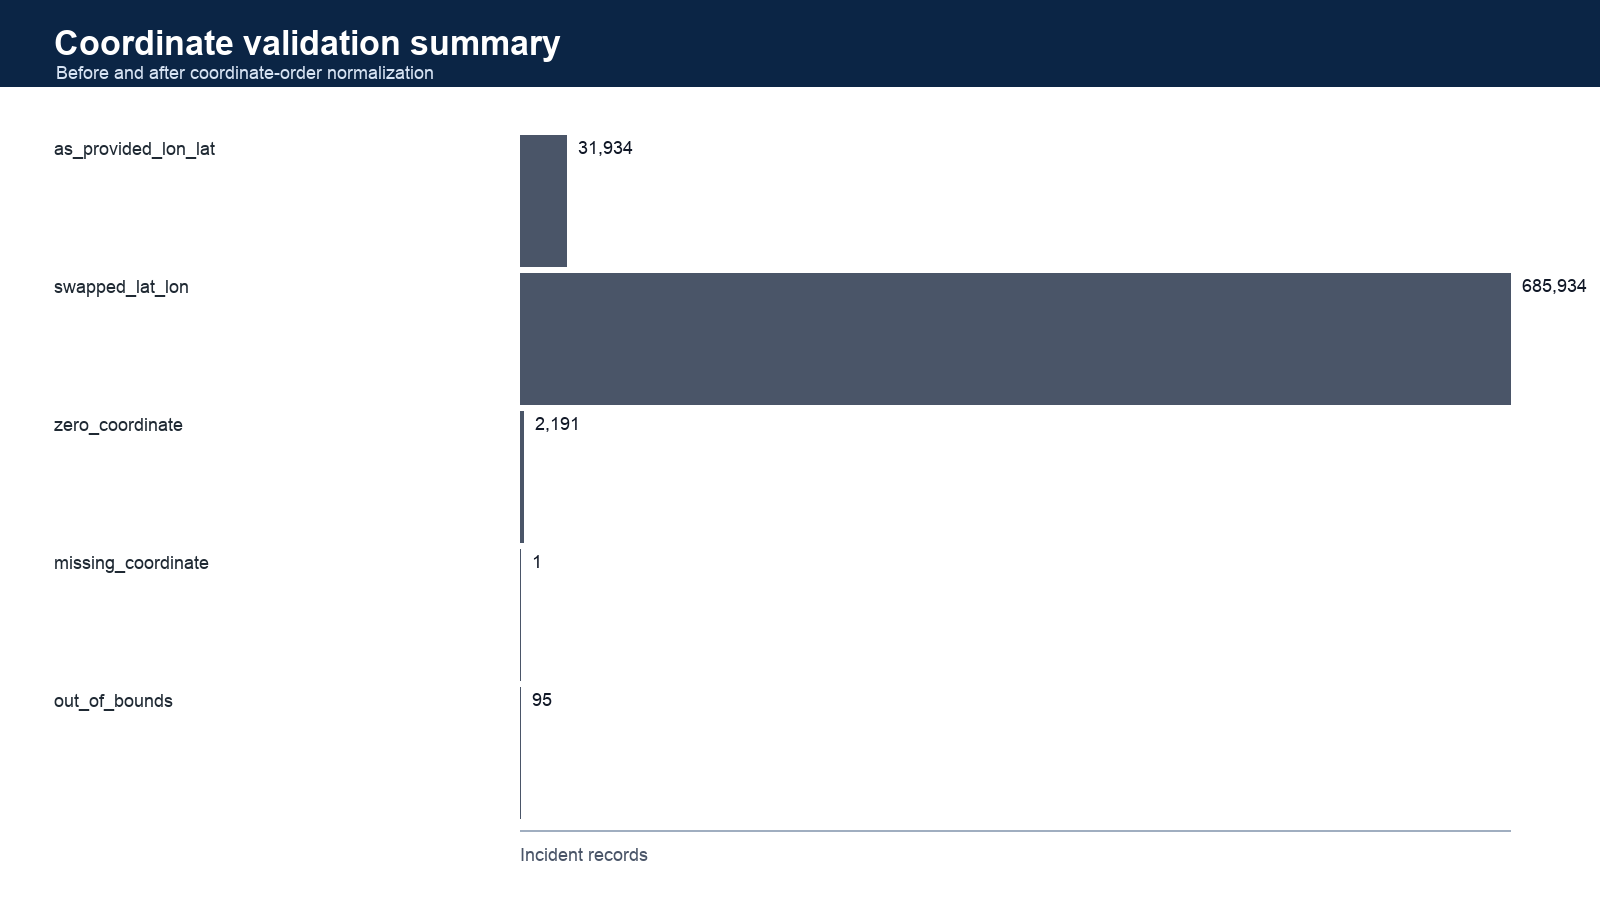
\includegraphics[width=0.82\textwidth]{coordinate_validation_summary.png}
\caption{Coordinate validation summary after raw coordinate audit and normalization.}
\label{fig:coordinate_validation_summary_final}
\end{figure}

This step is essential. Without coordinate normalization, most valid records would be assigned to incorrect locations, which would damage hotspot maps, H3 cell assignment, historical-risk priors, neighbor features, and dashboard maps.

\section{Exploratory data analysis}

After category exclusions, 719,729 rows remain for category and temporal EDA. The map-based EDA population is slightly smaller because it also requires valid normalized coordinates. The most common translated incident type is disabled vehicle on road, with 83,297 records. Thursday is the busiest day in the dataset with 110,569 incidents, and 14:00 is the busiest hour with 45,011 incidents.

\begin{table}[H]
\centering
\caption{Selected EDA findings}
\label{tab:selected_eda_findings}
\small
\begin{tabularx}{\textwidth}{L{0.36\textwidth}Y}
\toprule
\textbf{Metric} & \textbf{Finding} \\
\midrule
Raw records & 720,155 \\
Category/temporal EDA records & 719,729 \\
Map-usable rows & 717,615 \\
Top incident type & Disabled vehicle on road, 83,297 records \\
Top day of week & Thursday, 110,569 records \\
Top hour of day & 14:00, 45,011 records \\
Severity distribution & 82.22\% minor, 0.42\% moderate, 7.09\% severe, 10.27\% unknown \\
\bottomrule
\end{tabularx}
\end{table}

\begin{figure}[H]
\centering
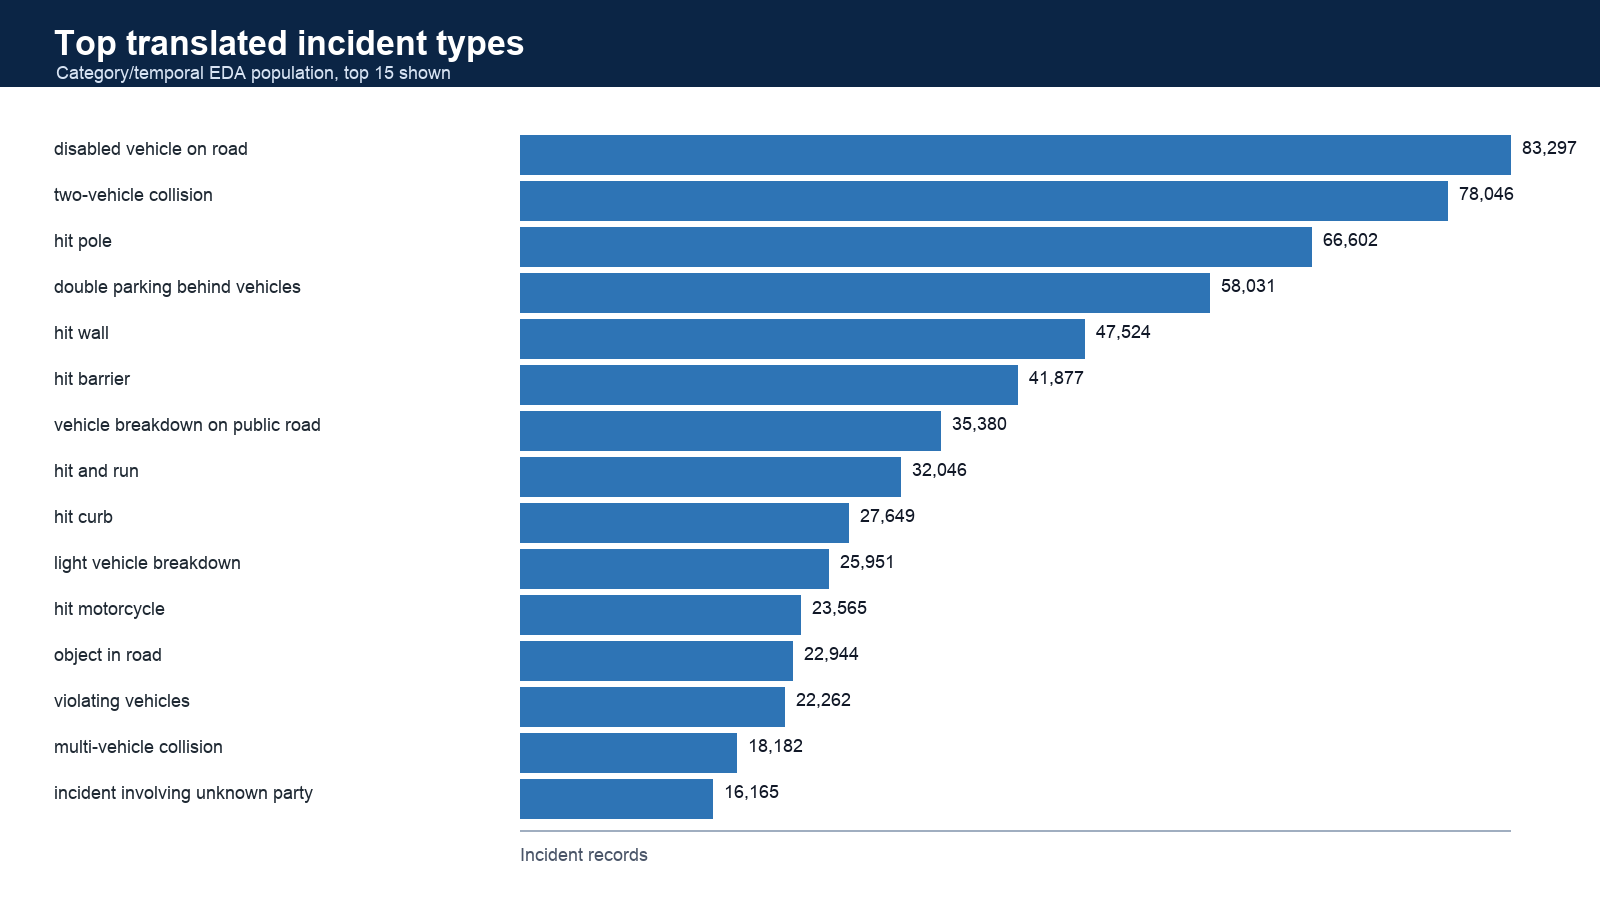
\includegraphics[width=0.92\textwidth]{top_incident_types.png}
\caption{Top translated incident types in the category/temporal EDA population.}
\label{fig:top_incident_types_final}
\end{figure}

The top categories show that the dataset is broader than an injury-crash file. It includes disabled vehicles, collisions, double parking, hit barriers, hit poles, hit walls, road objects, congestion, and related operational events. This supports the thesis title's focus on non-recurrent incident risk rather than only crash severity.

\begin{figure}[H]
\centering
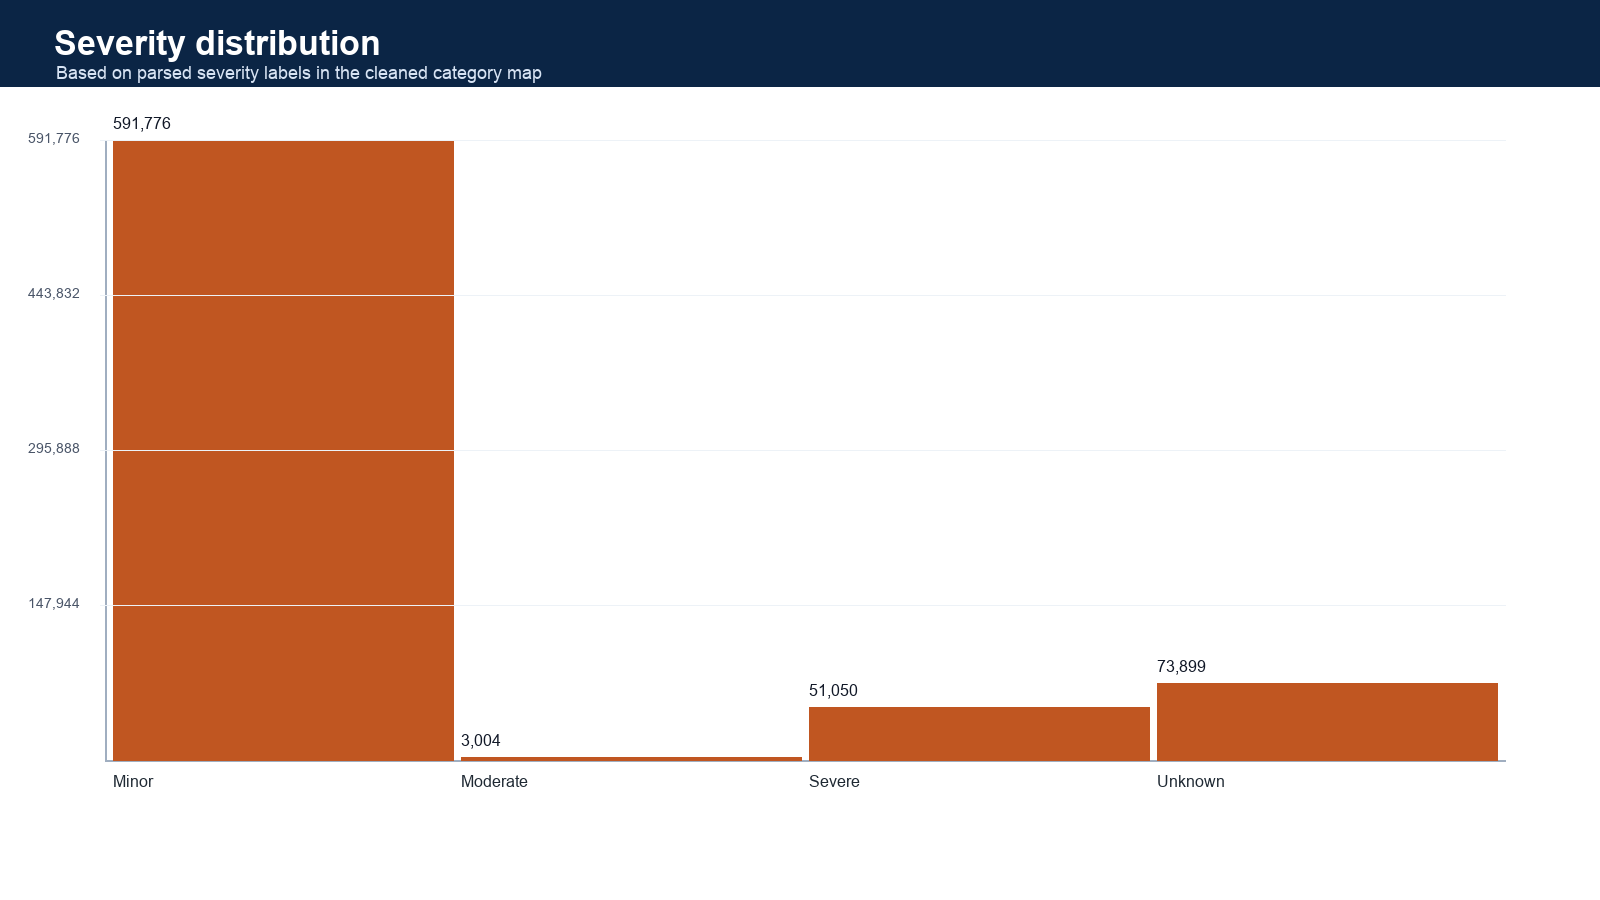
\includegraphics[width=0.78\textwidth]{severity_distribution.png}
\caption{Parsed severity distribution in the category/temporal EDA population.}
\label{fig:severity_distribution_final}
\end{figure}

The severity distribution is highly skewed toward minor incidents. There are 591,776 minor records, 3,004 moderate records, 51,050 severe records, and 73,899 unknown-severity records in the category/temporal EDA population. This supports keeping severity-aware analysis secondary. The main prediction target remains binary incident occurrence because the data contains many real incident reports without a fully specified severity label.

\begin{figure}[H]
\centering
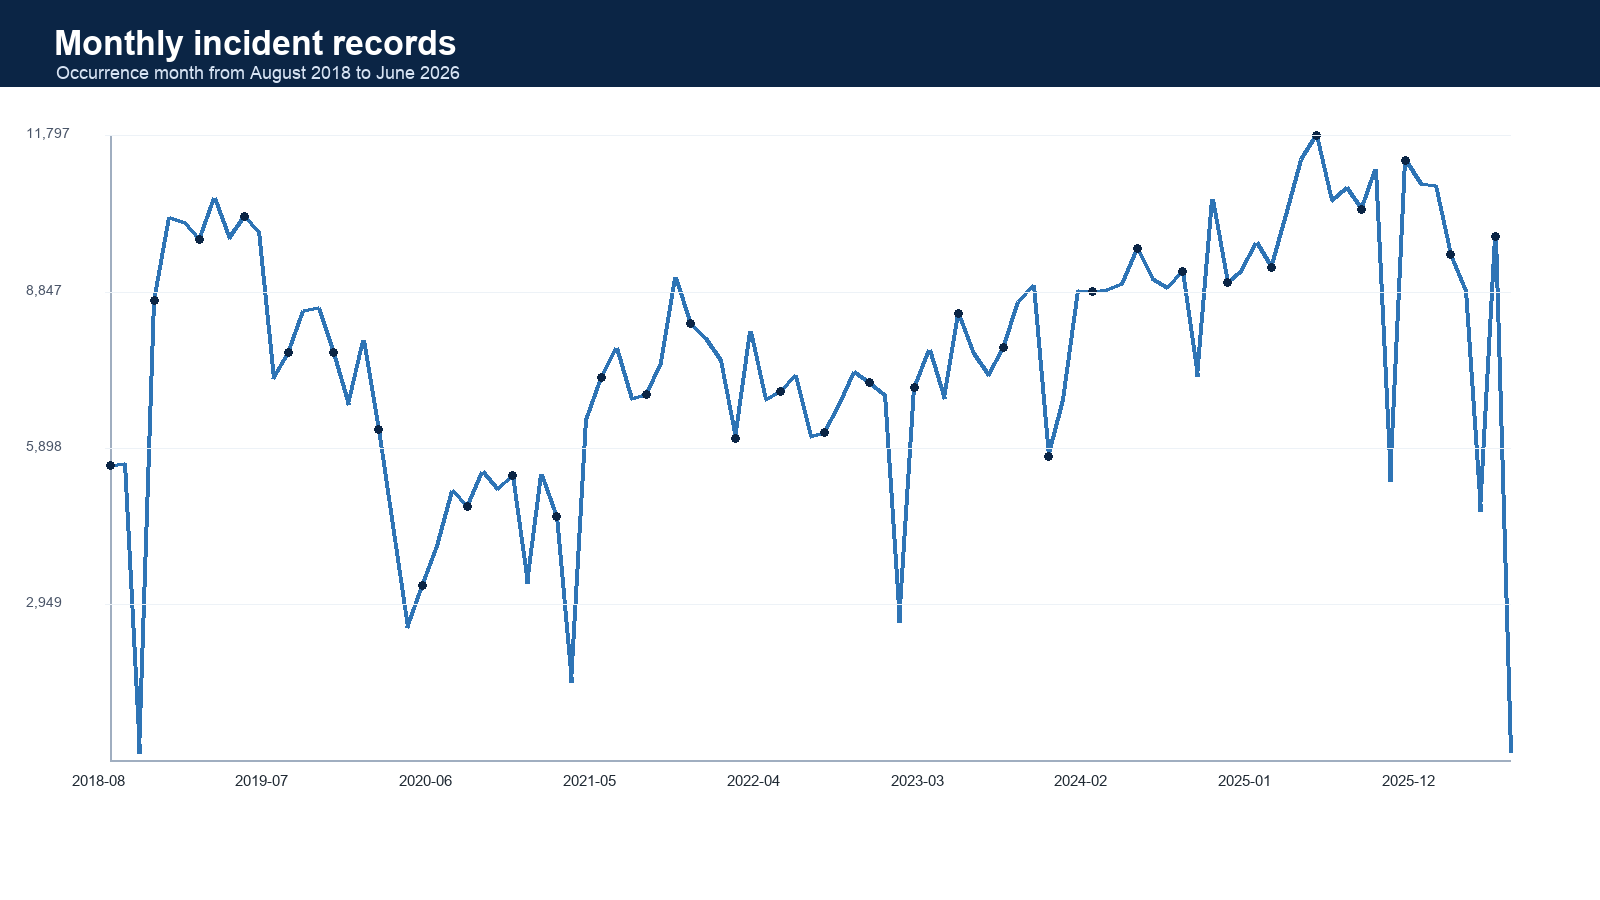
\includegraphics[width=0.88\textwidth]{monthly_incidents.png}
\caption{Monthly incident counts from August 2018 to June 2026.}
\label{fig:monthly_incidents_final}
\end{figure}

The monthly trend shows that incident reporting volume is not constant across the full period. Some early and final months are partial because the snapshot starts in August 2018 and ends on 1 June 2026. This is why chronological evaluation is more appropriate than random splitting: later periods should be treated as later periods, not randomly mixed with early data.

\begin{figure}[H]
\centering
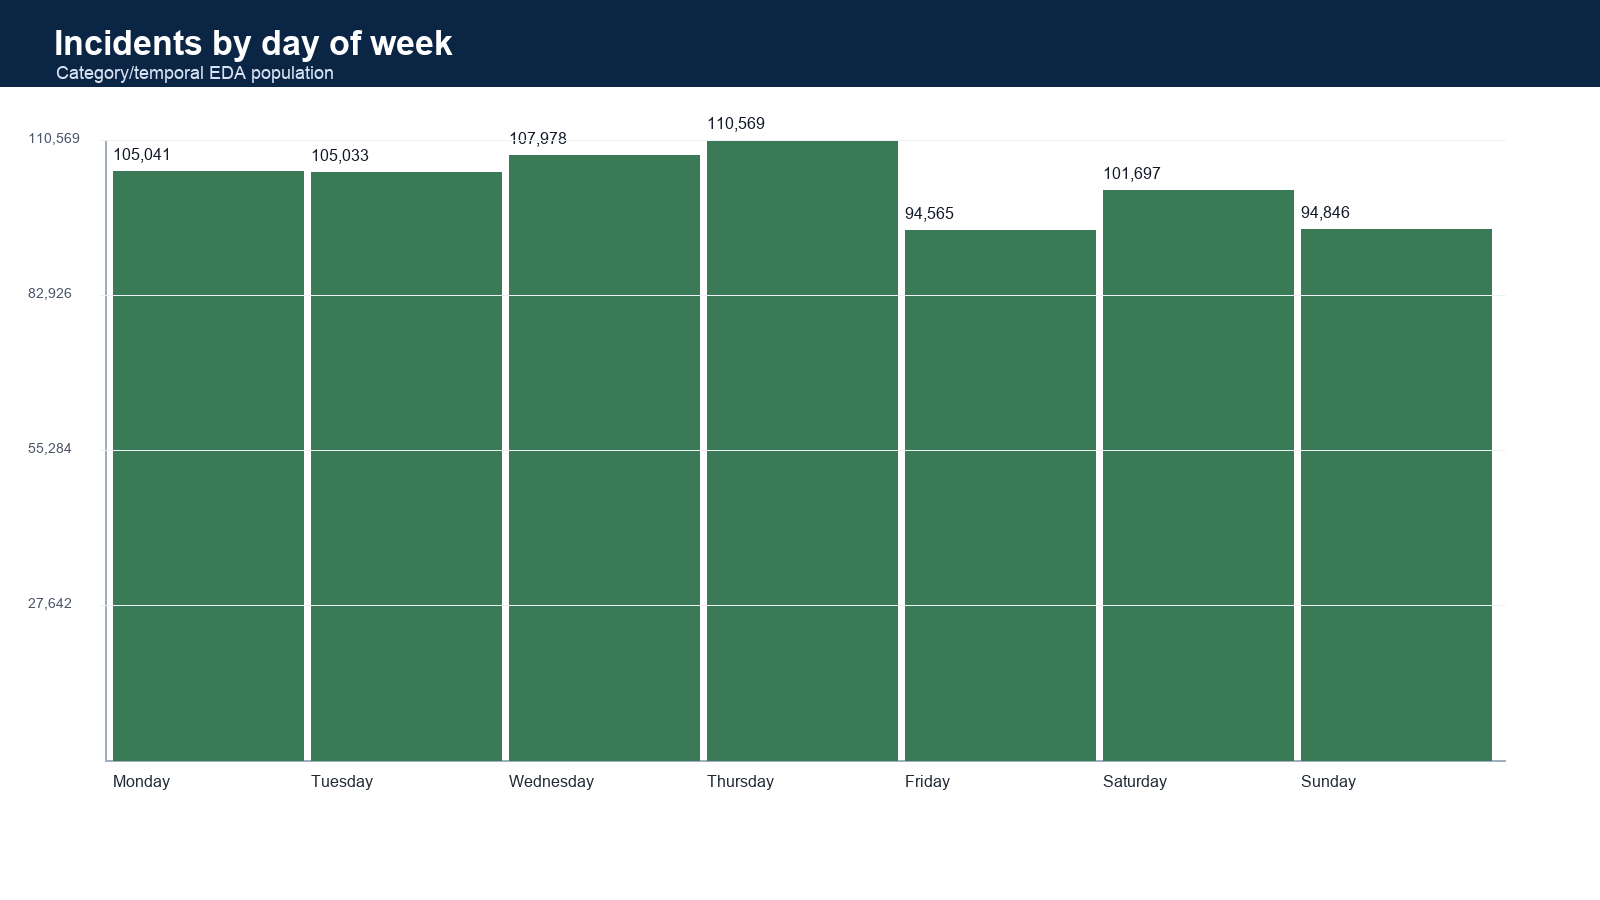
\includegraphics[width=0.78\textwidth]{day_of_week_incidents.png}
\caption{Incident counts by day of week.}
\label{fig:day_of_week_incidents_final}
\end{figure}

\begin{figure}[H]
\centering
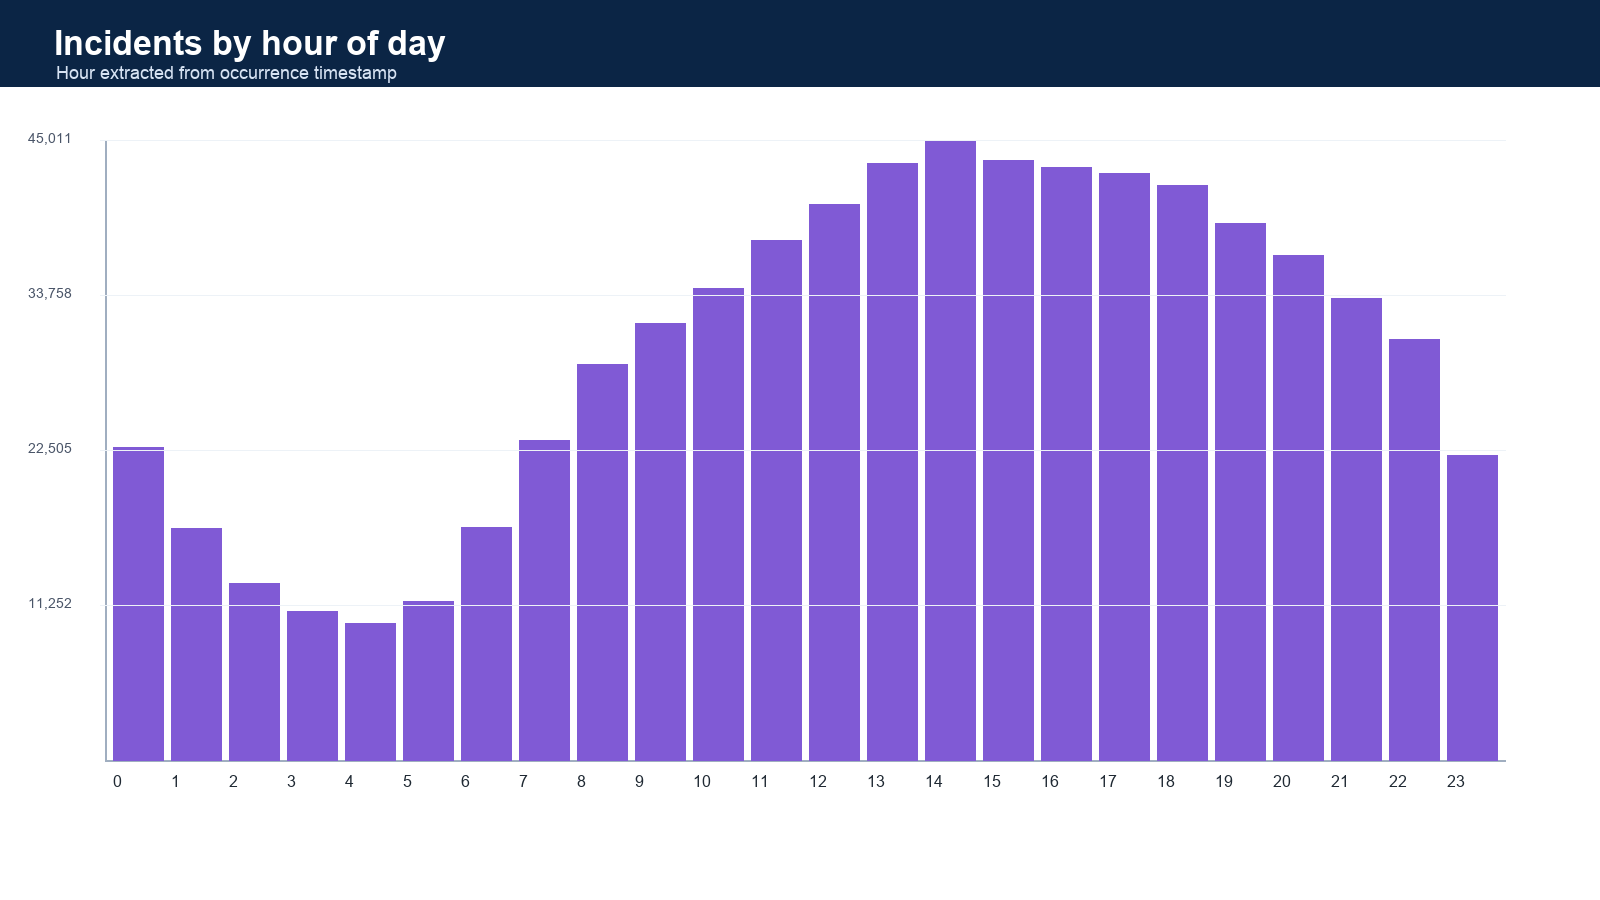
\includegraphics[width=0.78\textwidth]{hour_of_day_incidents.png}
\caption{Incident counts by hour of day.}
\label{fig:hour_of_day_incidents_final}
\end{figure}

The day-of-week and hour-of-day figures justify calendar features. They also make the task easier to explain: the model is not using a black-box timestamp. It uses explicit hour blocks, weekday patterns, weekend flags, month, and year, combined with historical and recent incident features.

\begin{figure}[H]
\centering
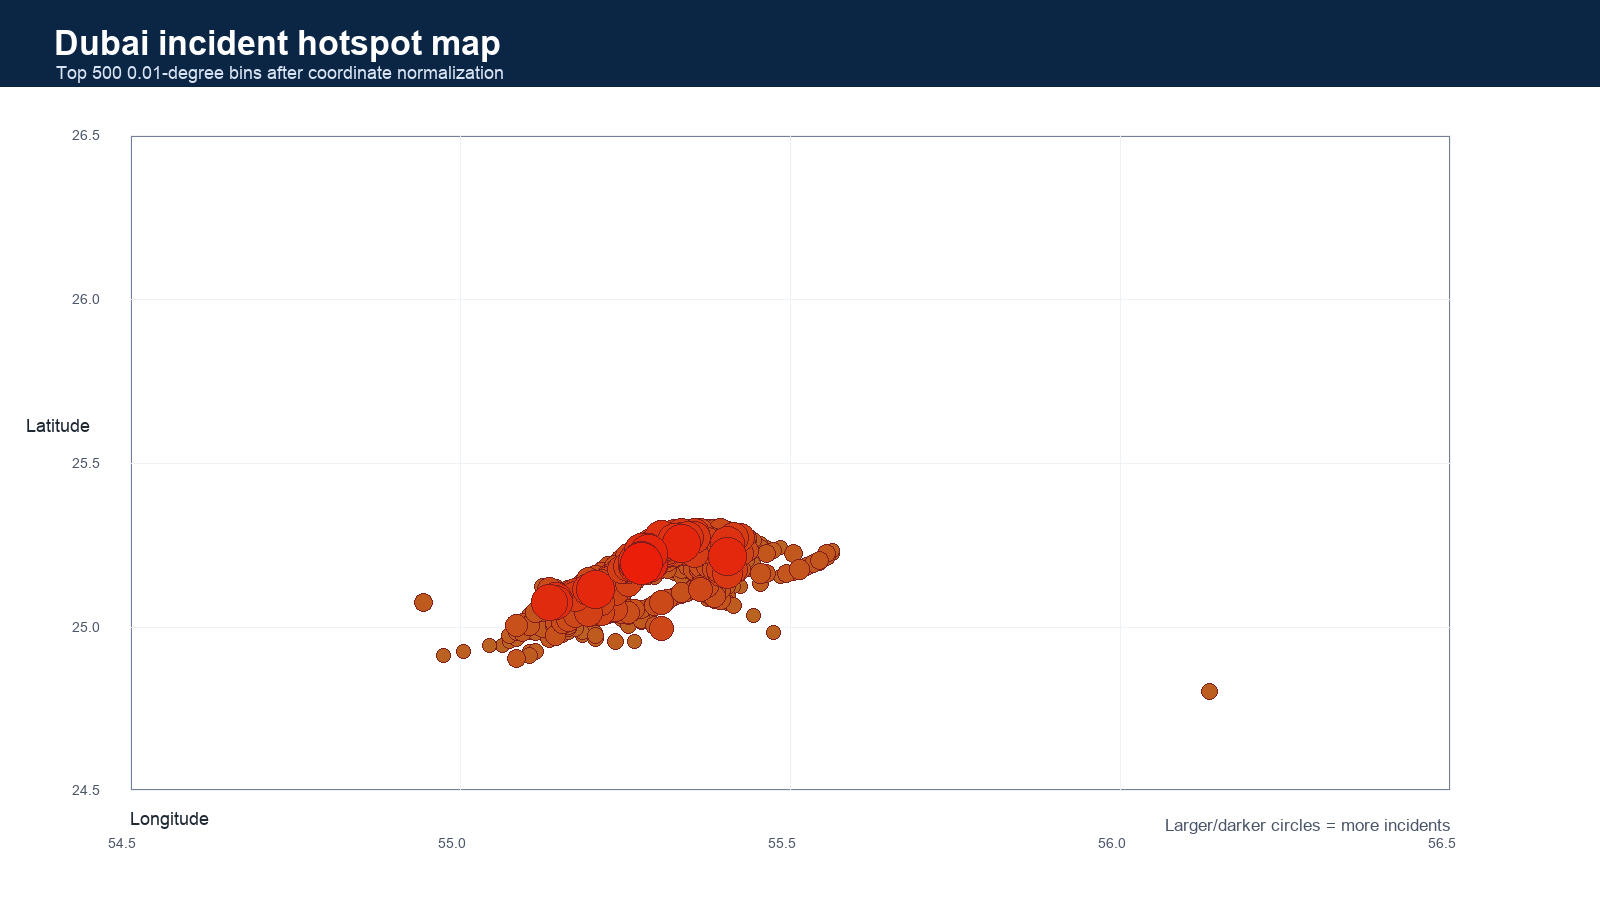
\includegraphics[width=0.86\textwidth]{dubai_hotspot_static.png}
\caption{Static Dubai hotspot plot using corrected coordinates.}
\label{fig:dubai_hotspot_static_final}
\end{figure}

The hotspot plot is a descriptive sanity check before modeling. It confirms that corrected coordinates place incidents in plausible Dubai locations. The final predictive maps use H3 cells and calibrated model scores rather than raw point-density bins.

\FloatBarrier

\section{H3 grid-time formulation}

The map-usable incidents are assigned to H3 cells. The main setting is H3 resolution 8 with 3-hour time windows. H3 was selected because it gives stable cell identifiers, supports neighbor queries, and works directly from coordinates. A Dubai boundary GeoJSON defines the main inside-Dubai cell universe. Peripheral observed cells and outside-UAE flags are retained in audits, but the final model and report focus on inside-Dubai cells.

H3 resolution 8 is a middle-scale choice. Coarser cells reduce sparsity but hide local spatial variation. Finer cells preserve more detail but make positives rarer and make the dashboard harder to read. The final sensitivity checks compare resolution 8 against coarser and finer settings before keeping it as the main thesis resolution.

The binary prediction target is:

\[
y_{z,t} =
\begin{cases}
1, & \text{if at least one incident occurs in H3 cell } z \text{ during window } t,\\
0, & \text{otherwise.}
\end{cases}
\]

Positive rows are observed incident cell/windows. Negative rows are cell/windows where no incident is observed. The negative rows are not raw records in the source file; they are constructed from the grid/time universe. This is why the model table can contain millions of rows even though the raw incident file contains 720,155 incident records.

\begin{table}[H]
\centering
\caption{Main H3 resolution-8, 3-hour grid-time dataset}
\label{tab:h3_grid_time_dataset}
\small
\begin{tabularx}{\textwidth}{L{0.40\textwidth}Y}
\toprule
\textbf{Item} & \textbf{Value} \\
\midrule
Map-usable incident points & 717,615 \\
Study-universe H3 cells before final inside-Dubai filtering & 3,584 \\
Inside-Dubai H3 cells for final evaluation & 1,305 \\
Positive grid-time rows & 678,174 \\
Sampled model rows & 4,069,044 \\
Negative sampling ratio & 5 negative rows per positive row \\
Window count & 22,795 \\
Window range & 13 August 2018 06:00 to 1 June 2026 12:00 \\
\bottomrule
\end{tabularx}
\end{table}

The first model sample contains all positive grid-time rows and five sampled negative rows for each positive row. Full-grid validation and test evaluation are then run on all inside-Dubai cells, not sampled negatives. This distinction is central to the results chapter.

\section{Chronological split}

The split is chronological. This is necessary because the model is meant to learn from earlier time windows and be evaluated on later time windows. A random row split would allow temporal patterns from later periods to appear in training and would make the result easier than the intended use case.

\begin{table}[H]
\centering
\caption{Inside-Dubai full-grid chronological split}
\label{tab:chronological_split}
\small
\begin{tabular}{lrrrr}
\toprule
\textbf{Split} & \textbf{Window indices} & \textbf{Candidate rows} & \textbf{Positive rows} & \textbf{Positive rate} \\
\midrule
Train & 0--15955 & 20,822,580 & 360,278 & 1.73\% \\
Validation & 15956--19374 & 4,461,795 & 104,435 & 2.34\% \\
Test & 19375--22794 & 4,463,100 & 108,224 & 2.42\% \\
\bottomrule
\end{tabular}
\end{table}

The validation and test periods have higher positive rates than the training period. This split drift is reported rather than hidden because it affects threshold selection, precision, recall, and dashboard interpretation. The model must be judged on the later period, not on a randomly mixed subset that would be easier to predict.

\chapter{Methodology}

The methodology is designed to keep the prediction task reproducible and defensible. The pipeline starts with cleaned incident records, constructs grid-time labels, builds only past-available features, compares simple and stronger models, and then explains the selected model.

This final report extends the mid-semester pipeline rather than replacing it. The same data audit, Arabic category translation, coordinate normalization, H3 grid construction, and chronological evaluation design are retained. The final stage adds neighbor-lag model selection, calibration, SHAP/LIME comparison, and the rolling-replay dashboard.

\section{Pipeline overview}

The complete pipeline has six stages:

\begin{enumerate}
    \item clean raw incident records, translate categories, and normalize coordinates;
    \item assign incidents to H3 cells and 3-hour windows;
    \item aggregate positive grid-time rows and construct negative grid-time rows;
    \item build leakage-safe temporal, lag, historical-risk, and neighboring-cell features;
    \item train and evaluate baseline and machine-learning models under chronological splits;
    \item calibrate and explain the selected model, then present it in a dashboard.
\end{enumerate}

The important design principle is that every model feature must be available before the target window begins. If a row represents cell \(z\) during window \(t\), the model may use information from earlier windows but not the incident count inside window \(t\). This rule is applied to same-cell lag features, neighboring-cell lag features, historical-risk priors, threshold selection, calibration, and dashboard replay.

\section{Prediction unit and label construction}

The prediction unit is an H3 cell/time-window pair. Let \(z\) denote an H3 cell and \(t\) denote a 3-hour window. The model row is \((z,t)\). The binary label is:

\[
y_{z,t} =
\begin{cases}
1, & \text{if one or more incidents occur in cell } z \text{ during window } t,\\
0, & \text{otherwise.}
\end{cases}
\]

This formulation creates two types of rows. A positive row means at least one cleaned incident point falls in that H3 cell during that window. A negative row means the cell and window exist in the evaluation universe but no incident is observed. The negative rows do not appear directly in the raw incident file; they are created by combining cells and time windows.

This is why the model sample is larger than the raw file. The raw file has 720,155 incident records. The H3/time construction creates 678,174 positive grid-time rows and many more possible negative cell/windows. The first training table keeps all positive rows and a 5:1 sampled set of negative rows, giving 4,069,044 model rows. Full-grid validation and test use every inside-Dubai cell/window candidate.

\section{Feature groups}

All model features are designed to be available before the target 3-hour window begins. Current-window incident counts, severity sums, and severity category counts are excluded from model inputs because they are part of the label being predicted.

\begin{table}[H]
\centering
\caption{Feature groups used in the final model path}
\label{tab:feature_groups}
\small
\begin{tabularx}{\textwidth}{L{0.27\textwidth}Y}
\toprule
\textbf{Feature group} & \textbf{Examples and purpose} \\
\midrule
Calendar features & Hour block, day of week, weekend flag, month, and year. These represent recurring temporal patterns. \\
Same-cell lag features & Previous 3-hour, 24-hour, and 7-day incident counts for the same H3 cell. These capture recent local activity. \\
Severity-weighted lag features & Previous 24-hour and 7-day known-severity weighted sums. Unknown severity contributes zero. \\
Historical-risk priors & Train-period empirical risk by cell-hour, cell, hour, and global rate. These capture long-run spatial and time-of-day risk. \\
Neighboring-cell lag features & Ring-1 H3 neighbor incident counts, severity-weighted sums, and active-cell counts. These capture nearby recent activity. \\
\bottomrule
\end{tabularx}
\end{table}

The calendar features are simple but important. The EDA shows that incident volume varies by hour and weekday. The lag features represent recent conditions in the same H3 cell. For example, a cell that had several incidents in the previous week may be more likely to be active again than a cell with no recent activity. Historical-risk priors represent long-term patterns learned from the training period only.

\section{Neighboring-cell feature design}

Neighboring cells are obtained from the H3 ring-1 neighborhood. The center cell is excluded, and only inside-Dubai cells are retained. This gives a simple spatial-neighborhood signal without requiring a full road-network graph.

The final neighbor features are:

\begin{itemize}
    \item previous 3-hour neighboring incident count;
    \item previous 24-hour neighboring incident count;
    \item previous 7-day neighboring incident count;
    \item previous 24-hour neighboring severity-weighted sum;
    \item previous 7-day neighboring severity-weighted sum;
    \item previous 24-hour active-neighbor-cell count;
    \item previous 7-day active-neighbor-cell count;
    \item number of inside-Dubai ring-1 neighbors retained for the cell.
\end{itemize}

These features are useful because incidents are not always isolated inside one hexagon. A nearby breakdown, obstruction, or collision may affect surrounding cells, and adjacent cells may share road corridors or activity patterns. The final report does not claim that H3 neighbors are the same as road-network neighbors. They are a reproducible spatial approximation that can be computed from the available data.

\section{Training design}

The first model training table uses all positive grid-time rows and a deterministic 5:1 sample of negative rows. This keeps training feasible while exposing the models to non-incident conditions. The final validation and test evaluation are not sampled. They score every inside-Dubai H3 cell for every validation or test 3-hour window.

This distinction matters. Sampled-negative results are useful for checking that the pipeline works, but they do not represent the real rarity of incident-positive cell/windows. The full-grid inside-Dubai evaluation is the main result because it uses the actual evaluation denominator: all candidate cells and windows in the selected spatial scope.

\begin{table}[H]
\centering
\caption{Training and evaluation populations}
\label{tab:training_evaluation_populations}
\small
\begin{tabularx}{\textwidth}{L{0.28\textwidth}L{0.22\textwidth}Y}
\toprule
\textbf{Population} & \textbf{Rows} & \textbf{Purpose} \\
\midrule
Sampled training table & 4,069,044 rows before later inside-Dubai filtering & Used for initial model training and the first sampled-negative baseline. \\
Inside-Dubai full-grid training universe & 20,822,580 candidate rows & Used to compute train-period historical-risk denominators. \\
Inside-Dubai full-grid validation & 4,461,795 candidate rows & Used for threshold selection and calibration fitting. \\
Inside-Dubai full-grid test & 4,463,100 candidate rows & Used once for final reported performance. \\
\bottomrule
\end{tabularx}
\end{table}

The training cap for XGBoost is 1,000,000 deterministic sampled rows. This cap keeps training feasible on a laptop while still using a large training sample. Validation and test are never capped in the full-grid experiments.

\section{Model families}

Four model families are compared.

\subsection{Historical risk baseline}

The historical risk baseline is the minimum serious baseline for this task. It estimates train-period empirical risk by H3 cell and hour block, with fallback rates where needed. If a specific cell-hour combination has little or no training history, the baseline falls back to broader cell-level, hour-level, and global rates.

This baseline is strong because the task is spatial and temporal. Some zones and time blocks are repeatedly active. A machine-learning model must therefore do more than rediscover that historically active cells remain risky.

\subsection{Logistic Regression}

Logistic Regression is used as a simple supervised baseline. It tests whether the engineered features contain predictive signal in a linear model. Numeric features are scaled, categorical features are one-hot encoded, and class balancing is used. Logistic Regression is not expected to capture complex nonlinear interactions, but it is useful because it is easier to interpret than tree ensembles.

\subsection{Random Forest}

Random Forest is a nonlinear tree ensemble. It can capture interactions between calendar variables, historical risk, and lag counts. It is included as a stronger baseline before XGBoost. The training run uses a deterministic cap because fitting large forests on the full sampled table is heavier than fitting the linear model.

\subsection{XGBoost}

XGBoost is the selected model family for the final pipeline. It is a gradient-boosted tree method suited to structured tabular data \cite{chen2016xgboost}. It can model nonlinear interactions, works well with engineered historical and lag features, and integrates cleanly with SHAP explanations. LightGBM is reviewed as a related boosted-tree framework \cite{ke2017lightgbm}, but the final implementation uses XGBoost because it was already integrated with the full-grid evaluation, calibration, SHAP, LIME, and dashboard workflow.

\section{Leakage controls}

The main leakage risk is using information from the target window or later periods when building features. The model must predict whether a cell/window will contain an incident, so the current-window incident count and severity statistics cannot be predictors.

\begin{table}[H]
\centering
\caption{Leakage controls used in modeling}
\label{tab:leakage_controls}
\small
\begin{tabularx}{\textwidth}{L{0.30\textwidth}Y}
\toprule
\textbf{Leakage risk} & \textbf{Control used} \\
\midrule
Current-window incident counts used as features & \texttt{incident\_count}, severity sums, and severity count columns are excluded from model inputs. \\
Future temporal patterns used in training & Train, validation, and test splits are chronological. Random K-fold is not used as the main validation design. \\
Historical-risk priors computed from future periods & Main historical priors are computed from the training period; an expanding-history audit checks whether training-row historical priors materially change the result. \\
Lag features using the current window & Previous-window features are computed from windows before the target window only. \\
Hard-negative mining from validation/test & Hard negatives are mined only from training-window negatives. Validation and test remain untouched. \\
Calibration fitted on test labels & Sigmoid and isotonic calibration are fitted only on validation predictions and labels. \\
Dashboard forecasting beyond data cutoff & Active dashboard uses rolling replay. Later forecasts require updated incident records because recent lag features are unavailable after 1 June 2026. \\
\bottomrule
\end{tabularx}
\end{table}

Random K-fold cross-validation is not used as the main result. In a time-indexed risk task, random folds would mix earlier and later windows. The model could learn temporal patterns from future windows and then appear stronger when evaluated on earlier rows. If a later robustness check is added, it should use blocked or rolling time-series cross-validation rather than random K-fold.

\section{Model-improvement experiments}

After the first full-grid evaluation, four improvement or robustness checks are run:

\begin{enumerate}
    \item \textbf{Historical-risk audit}: compare full features, expanding training-history priors, no historical-risk features, temporal-lag-only features, temporal-only features, and historical score only.
    \item \textbf{H3/time-window sensitivity}: compare H3 resolution 7, 8, and 9, and 1-hour, 3-hour, and 6-hour window choices.
    \item \textbf{Neighboring-cell lag features}: add ring-1 H3 neighbor history and compare against the current XGBoost feature set.
    \item \textbf{Hard-negative and tuning experiments}: test whether a harder negative training sample or tuned XGBoost hyperparameters improve the untouched full-grid test result.
\end{enumerate}

The experiments are ordered deliberately. The full-grid result comes before model improvement so that the project has a realistic evaluation denominator. The historical-risk audit checks whether the model is mainly historical memorization. Sensitivity checks test whether the chosen grid/time setting is defensible. Neighbor features are added only after the main pipeline works. Hard-negative training and tuning are treated as experiments, not automatically accepted improvements.

\section{Evaluation metrics}

The report uses ROC-AUC, PR-AUC, precision, recall, F1, confusion matrices, and top-k hotspot metrics. PR-AUC is emphasized because incident-positive cell/windows are rare \cite{saito2015prauc}. Accuracy is not emphasized because a model that predicts every cell/window as negative would look accurate in a rare-event task while being useless for hotspot detection.

ROC-AUC measures whether the model tends to score positive rows above negative rows across thresholds. PR-AUC focuses on precision and recall, so it is more sensitive to rare positives. F1 is the harmonic mean of precision and recall at the selected threshold. Recall measures how many true positive cell/windows are captured. Precision measures how many predicted positive cell/windows actually contain incidents.

Top-k hotspot metrics answer a different question. For each test time window, the model ranks all inside-Dubai cells by risk. The top-k metric checks whether the highest-ranked cells contain actual incidents. This is closer to how a traffic analyst might inspect the model output: the analyst may care about the top 5, 10, or 20 zones per time block rather than a binary decision for every cell in the city.

\section{Calibration}

The selected XGBoost score is calibrated before dashboard display. Calibration does not change the ranking model; it post-processes scores so the displayed risk value is closer to an observed probability. Sigmoid calibration and isotonic calibration are fitted on validation predictions only. The test set is used for final reporting.

Calibration is needed because a raw machine-learning probability can be poorly calibrated even when it ranks cells well. A score of 0.80 should not be displayed as an 80\% risk unless the observed rate in similar scored cases is close to 80\%. The calibration experiment shows that the uncalibrated XGBoost score is useful for ranking but too confident as a probability. Sigmoid calibration is therefore used for dashboard risk display.

\section{Explainability}

SHAP is the main explanation method because it provides global and local feature attributions for the selected XGBoost model \cite{lundberg2017shap}. LIME is used as a local model-agnostic comparison on selected examples \cite{ribeiro2016lime}. The explanations describe how the model uses available features. They do not prove that a feature causes an incident.

The SHAP global output ranks feature groups by average contribution magnitude. This shows whether the model is mainly using historical cell-hour risk, recent incident history, neighboring-cell history, calendar variables, or other engineered features. The SHAP local output explains one selected prediction by showing which features pushed the score up or down. LIME is used on the same local cases to check whether a different explanation method points to similar drivers.

The final dashboard uses SHAP for selected-zone explanations because SHAP can be computed consistently for the final tree model and can be shown as top reasons with contribution bars. LIME remains in the report as a supporting local comparison.

\chapter{Results and discussion}

This chapter presents the final experimental story. The first sampled-negative models showed that the pipeline worked, but the main evidence comes from inside-Dubai full-grid validation and test scoring. The final model path is selected only after checking the historical-risk features, H3/time-window choices, neighboring-cell lag features, hard-negative training, XGBoost tuning, calibration, and explainability.

\begin{table}[H]
\centering
\caption{Completed experiments and final decisions}
\label{tab:completed_experiments_decisions}
\footnotesize
\begin{tabularx}{\textwidth}{L{0.28\textwidth}L{0.30\textwidth}Y}
\toprule
\textbf{Experiment} & \textbf{Purpose} & \textbf{Decision in final report} \\
\midrule
Sampled-negative baseline & Check the end-to-end supervised-learning pipeline with historical risk, Logistic Regression, Random Forest, and XGBoost. & Kept as an initial pipeline check, not the final performance denominator. \\
Inside-Dubai full-grid evaluation & Evaluate all inside-Dubai H3 cells in validation and test windows. & Used as the main model-selection evidence. XGBoost was strongest among the first full-grid models. \\
Historical-risk audit & Test whether historical-risk features dominate or create training-time leakage. & Kept historical priors. Expanding-history results were almost unchanged, reducing leakage concern. \\
H3/time-window sensitivity & Compare H3-7, H3-8, H3-9 and 1-hour, 3-hour, 6-hour windows. & Kept H3-8 with 3-hour windows as the main balance of detail, sparsity, and dashboard practicality. \\
Neighboring-cell lag features & Test whether ring-1 H3 neighbor history improves prediction. & Promoted. Neighbor lags improved PR-AUC, F1, and top-20 incident capture modestly. \\
Hard-negative training & Test whether high-scoring training negatives improve the selected model. & Rejected. It reduced full-grid PR-AUC, F1, and hotspot capture. \\
XGBoost tuning & Tune the neighbor-feature XGBoost model using validation-only selection. & Rejected. The tuned model did not improve the untouched test result. \\
Sigmoid calibration & Make displayed risk scores more reliable for the dashboard. & Promoted for probability display. Ranking metrics were preserved and Brier score improved. \\
SHAP/LIME explanations & Explain the final model globally and locally. & SHAP is the main explanation method. LIME is retained as a supporting local comparison. \\
Dashboard & Present where, when, and why the model ranks zones as risky. & Implemented as a rolling replay using the final neighbor-feature XGBoost model, English dashboard map, and SHAP reasons. \\
\bottomrule
\end{tabularx}
\end{table}

\section{Initial sampled-negative baseline}

The first baseline used the 5:1 sampled model table. It compared historical risk, Logistic Regression, Random Forest, and XGBoost on the initial modeling population. These results were useful for checking the end-to-end pipeline, but they are not the final evaluation denominator because the test negatives were sampled.

This stage answered a practical question: after the data audit, H3 conversion, feature engineering, and chronological split, can the supervised-learning pipeline train and score models without leakage columns? The sampled-negative table is useful for this purpose because it contains all positive rows and enough negative rows to train the first models. It is not the final performance claim because the negative class is artificially reduced.

\begin{table}[H]
\centering
\caption{Initial sampled-negative baseline result}
\label{tab:initial_sampled_negative_baseline}
\small
\begin{tabular}{lrrrr}
\toprule
\textbf{Model} & \textbf{ROC-AUC} & \textbf{PR-AUC} & \textbf{Recall} & \textbf{F1} \\
\midrule
Historical risk & 0.8850 & 0.6387 & 0.7403 & 0.6437 \\
Logistic Regression & 0.8847 & 0.6442 & 0.7405 & 0.6439 \\
Random Forest & 0.8904 & 0.6542 & 0.7420 & 0.6473 \\
XGBoost & 0.8899 & 0.6544 & 0.7437 & 0.6471 \\
\bottomrule
\end{tabular}
\end{table}

The sampled-negative PR-AUC values are much higher than the full-grid PR-AUC values because the sampled table contains many fewer non-incident cell/windows than the real full grid. This is why the report treats the sampled-negative baseline as a pipeline check rather than the final performance claim.

The tree-based models are slightly stronger than the historical and linear baselines in the sampled table, but the gap is not large. This already suggested that historical location/time risk is a strong signal. It also showed that the final evaluation needed a harder denominator. A good score on sampled negatives does not prove that the model can rank all inside-Dubai cells in later windows.

\begin{figure}[H]
\centering
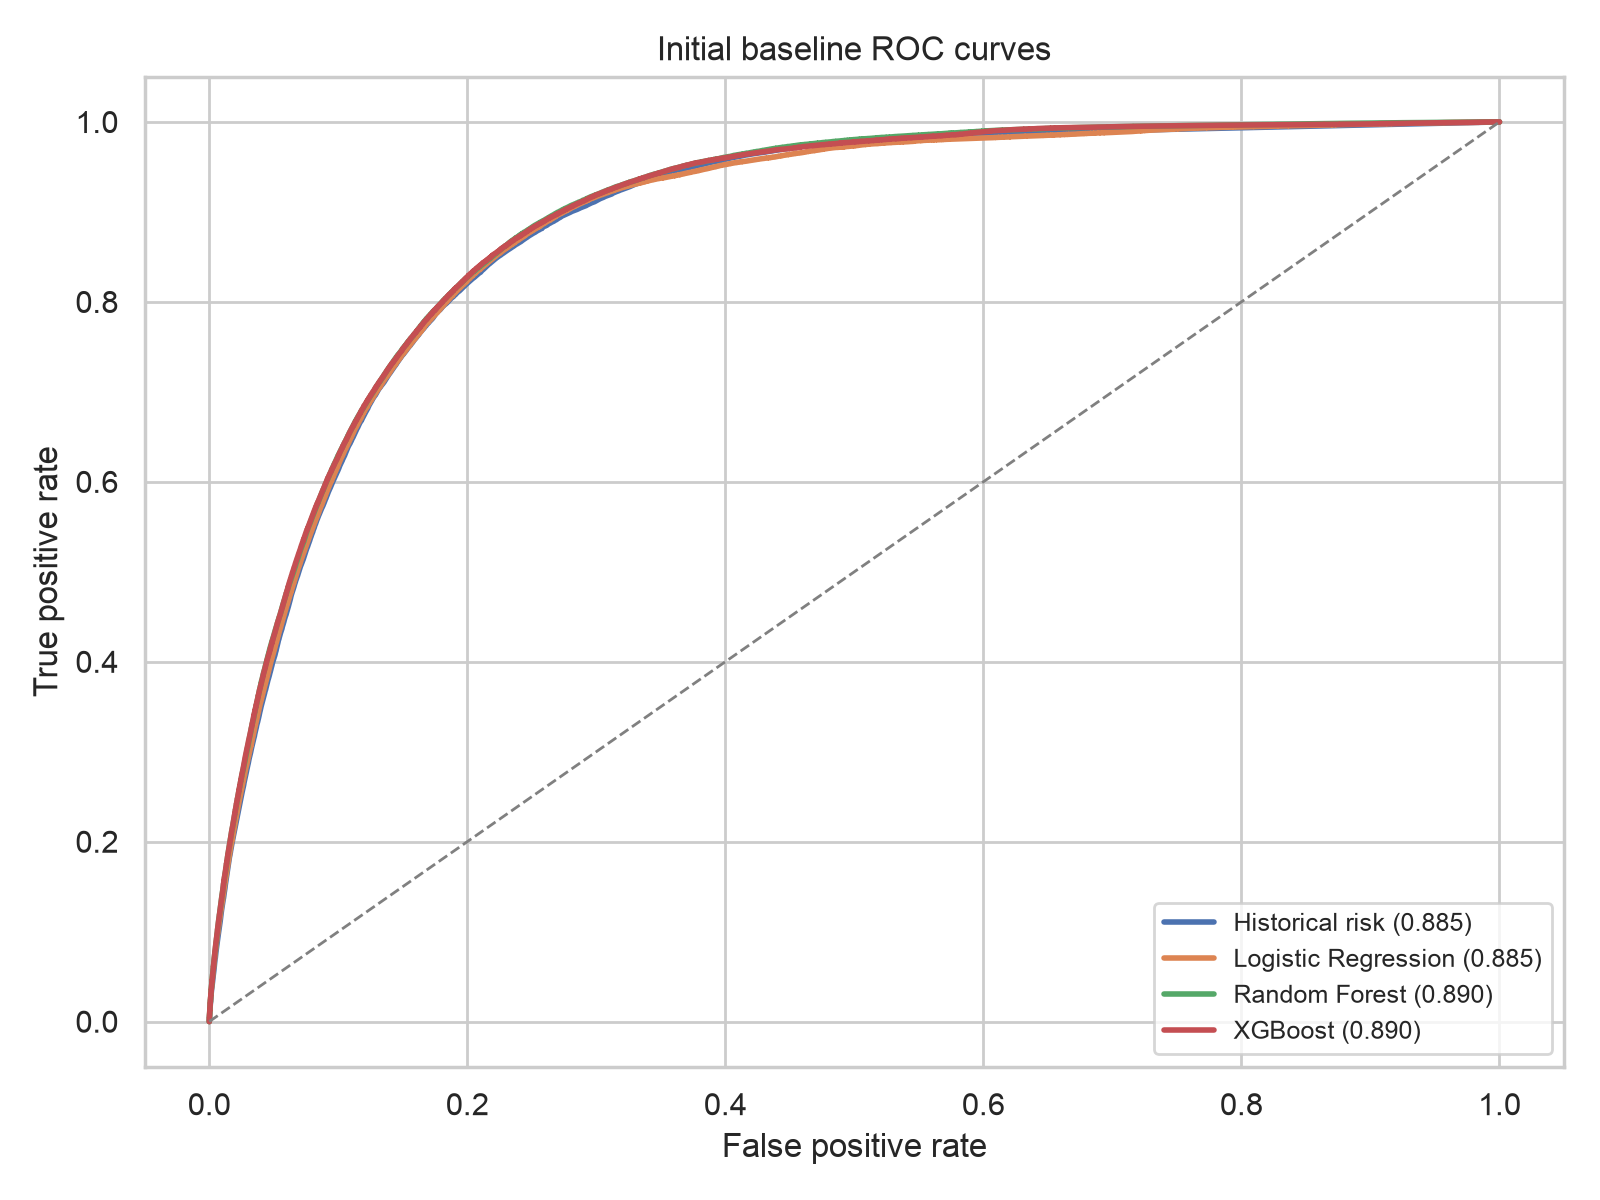
\includegraphics[width=0.86\textwidth]{initial_baseline_roc_curve.png}
\caption{ROC curves for the initial sampled-negative baseline.}
\label{fig:initial_baseline_roc_curve_final}
\end{figure}

\begin{figure}[H]
\centering
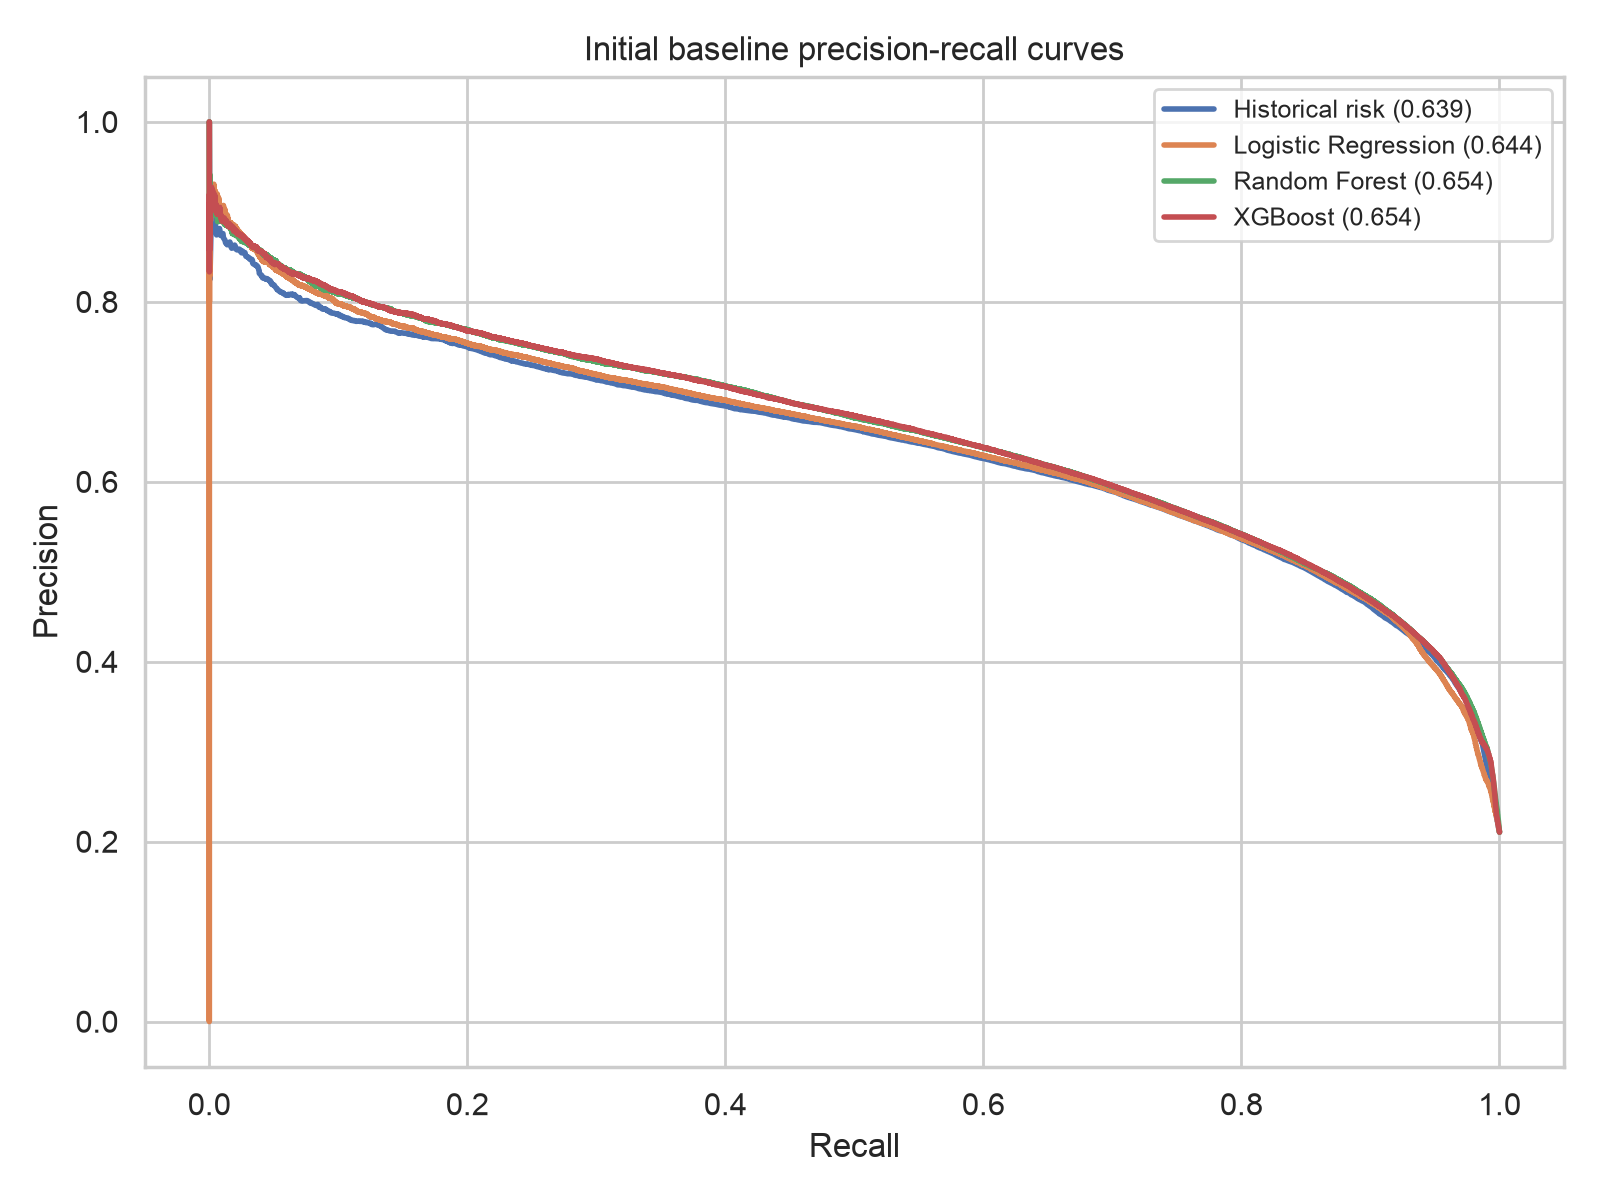
\includegraphics[width=0.86\textwidth]{initial_baseline_pr_curve.png}
\caption{Precision-recall curves for the initial sampled-negative baseline.}
\label{fig:initial_baseline_pr_curve_final}
\end{figure}

\FloatBarrier

\section{Inside-Dubai full-grid evaluation}

The main evaluation uses the inside-Dubai H3 resolution-8, 3-hour full grid. The test period contains 4,463,100 candidate cell/windows, of which 108,224 are positive. The base incident-positive rate is therefore 2.42\%. This rare-event setting makes PR-AUC and top-k hotspot metrics more meaningful than accuracy.

\begin{table}[H]
\centering
\caption{Inside-Dubai full-grid baseline result}
\label{tab:final_full_grid_baseline}
\small
\begin{tabular}{lrrrrr}
\toprule
\textbf{Model} & \textbf{ROC-AUC} & \textbf{PR-AUC} & \textbf{Precision} & \textbf{Recall} & \textbf{F1} \\
\midrule
Historical risk & 0.7990 & 0.0882 & 0.1063 & 0.2679 & 0.1522 \\
Logistic Regression & 0.7995 & 0.0932 & 0.1087 & 0.2792 & 0.1565 \\
Random Forest & 0.8062 & 0.0954 & 0.1133 & 0.2721 & 0.1599 \\
XGBoost & 0.8067 & 0.0967 & 0.1165 & 0.2630 & 0.1615 \\
\bottomrule
\end{tabular}
\end{table}

XGBoost is the strongest model in the first full-grid comparison. The improvement over historical risk is modest but consistent: PR-AUC improves from 0.0882 to 0.0967, and F1 improves from 0.1522 to 0.1615. This is expected because historical cell/time risk is already a strong predictor for this task.

The full-grid result is much more conservative than the sampled-negative result. Test PR-AUC falls from about 0.65 in the sampled table to about 0.10 in the full-grid setting. This does not mean the model failed. It means the evaluation denominator changed to the true city grid, where most cell/windows do not contain incidents. In this setting, even a small PR-AUC improvement over historical risk is meaningful if it also improves top-k hotspot ranking.

\begin{table}[H]
\centering
\caption{Inside-Dubai full-grid top-20 hotspot ranking}
\label{tab:final_full_grid_top20}
\footnotesize
\begin{tabular}{lrrrr}
\toprule
\textbf{Model} & \textbf{Pos. cells} & \textbf{Prec.@20} & \textbf{Hit@20} & \textbf{Incidents} \\
\midrule
Historical risk & 8,847 & 0.1293 & 0.9106 & 10,043 \\
Logistic Regression & 8,994 & 0.1315 & 0.9103 & 10,227 \\
Random Forest & 8,946 & 0.1308 & 0.9122 & 10,186 \\
XGBoost & 9,049 & 0.1323 & 0.9183 & 10,281 \\
\bottomrule
\end{tabular}
\end{table}

The top-k result is a hotspot-ranking result, not a proof that every future incident can be located. It asks whether the highest-ranked cells in each test window contain incidents. XGBoost captures the most top-20 incidents in the first full-grid evaluation.

The top-k comparison is especially important for defending the model. A traffic-risk dashboard is unlikely to ask a user to inspect all 1,305 cells in every 3-hour window. It is more realistic to rank cells and inspect the highest-risk zones. The top-20 result shows that XGBoost captures 10,281 incidents in the highest-ranked cells across the test period, compared with 10,043 for historical risk. The gain is modest, but it is consistent with the PR-AUC and F1 improvement.

\begin{figure}[H]
\centering
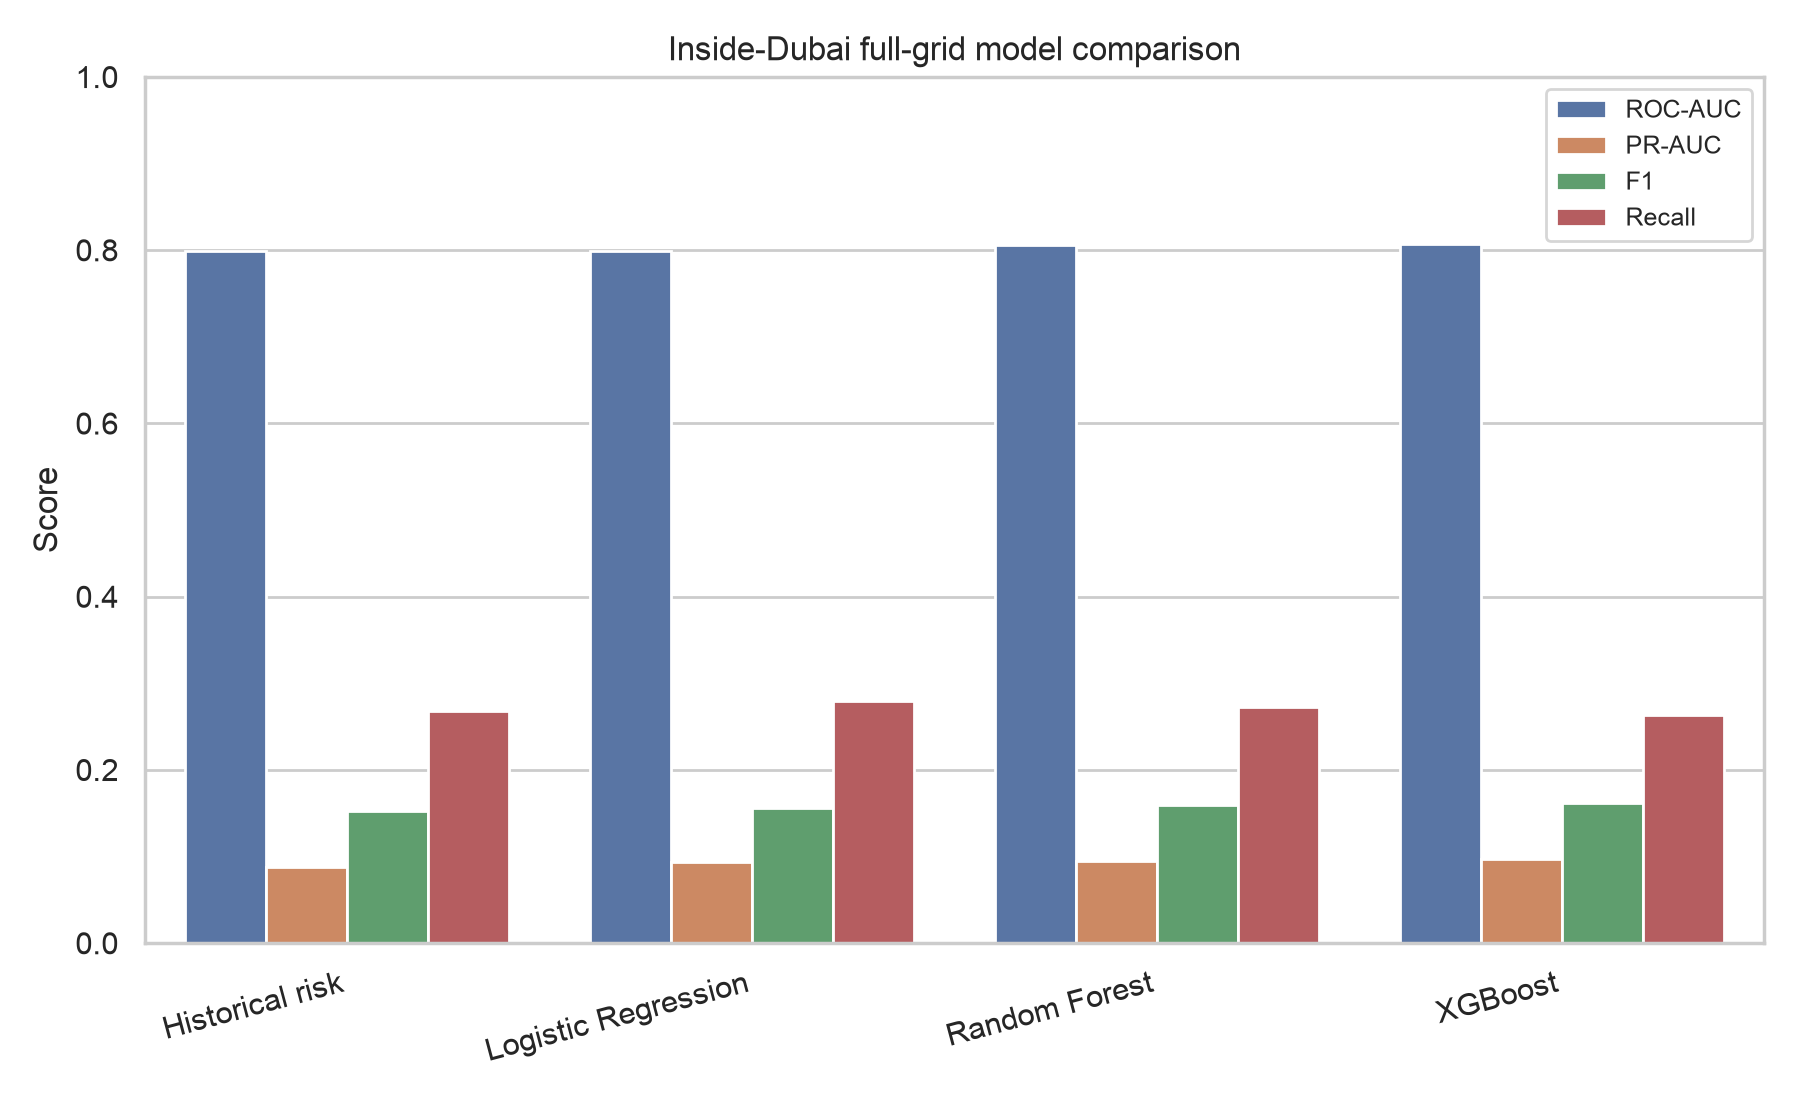
\includegraphics[width=0.88\textwidth]{final_full_grid_model_comparison.png}
\caption{Inside-Dubai full-grid model comparison}
\label{fig:final_full_grid_model_comparison}
\end{figure}

\begin{figure}[H]
\centering
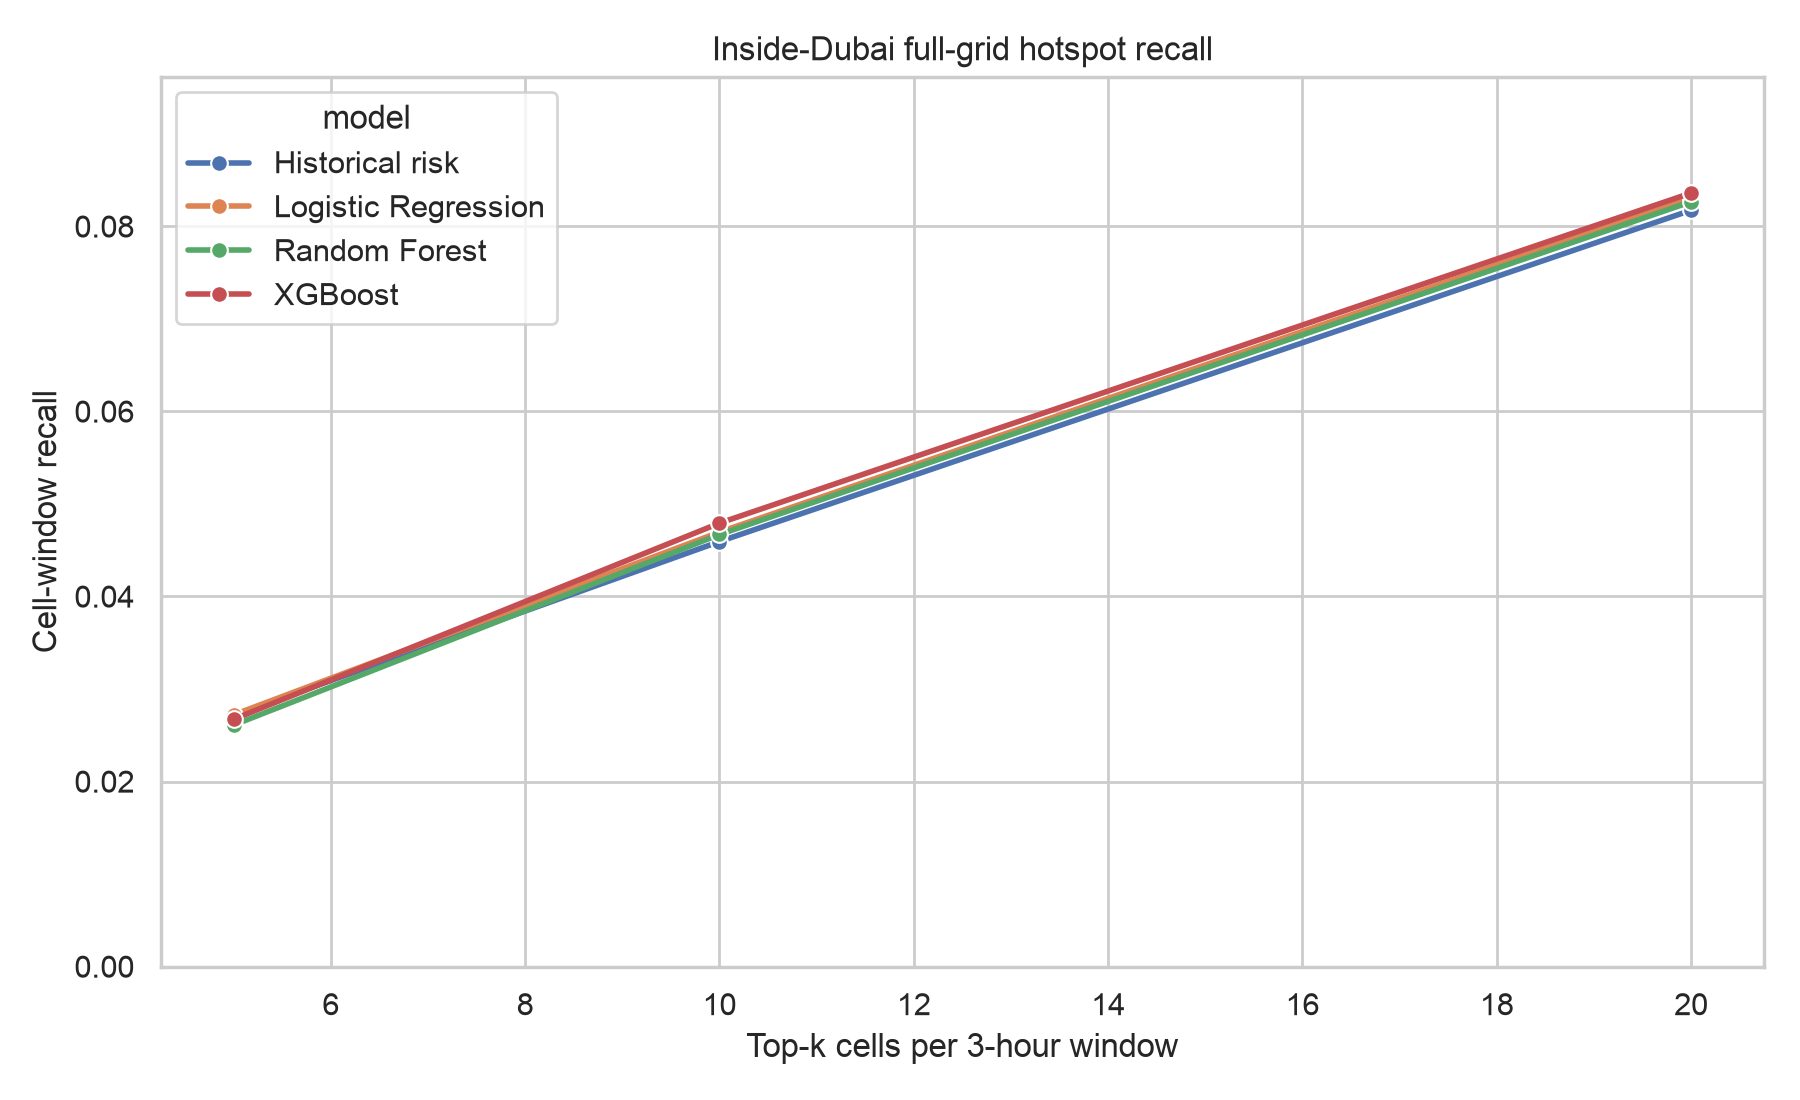
\includegraphics[width=0.88\textwidth]{final_full_grid_topk_comparison.png}
\caption{Inside-Dubai full-grid top-k hotspot comparison}
\label{fig:final_full_grid_topk_comparison}
\end{figure}

\FloatBarrier

\section{Historical-risk feature audit}

Because historical cell/time risk is expected to be strong, an audit was run to check whether model performance depends mainly on those features and whether the train-period historical priors create a leakage concern. The audit compares the full XGBoost feature set, an expanding-training-history variant, versions without historical-risk features, temporal-only features, and a historical-score-only baseline.

\begin{table}[H]
\centering
\caption{Historical-risk feature audit}
\label{tab:historical_risk_audit}
\small
\begin{tabular}{lrrrr}
\toprule
\textbf{Feature set} & \textbf{ROC-AUC} & \textbf{PR-AUC} & \textbf{Recall} & \textbf{F1} \\
\midrule
All features, train-period history & 0.8067 & 0.0967 & 0.2630 & 0.1615 \\
All features, expanding train history & 0.8066 & 0.0963 & 0.2649 & 0.1613 \\
No historical-risk features & 0.7757 & 0.0843 & 0.2761 & 0.1498 \\
Temporal and lag only & 0.7760 & 0.0850 & 0.2713 & 0.1501 \\
Temporal only & 0.5983 & 0.0311 & 0.4794 & 0.0615 \\
Historical score only & 0.7990 & 0.0882 & 0.2679 & 0.1522 \\
\bottomrule
\end{tabular}
\end{table}

Removing historical-risk features reduces PR-AUC from 0.0967 to 0.0843 and F1 from 0.1615 to 0.1498. Historical priors therefore matter. The expanding-history check is almost identical to the train-period historical-prior result, which reduces the concern that the reported performance is an artifact of training-time historical-risk leakage.

The audit also clarifies the role of the model. The XGBoost model is not discovering risk from calendar variables alone. Temporal-only features give PR-AUC 0.0311 and F1 0.0615, which is much weaker than the full model. Same-cell and lag features improve the result, but the long-term cell/hour historical prior remains central. This is reasonable for incident-risk prediction because road layout, land use, traffic generators, and reporting patterns are partly stable over time.

\begin{figure}[H]
\centering
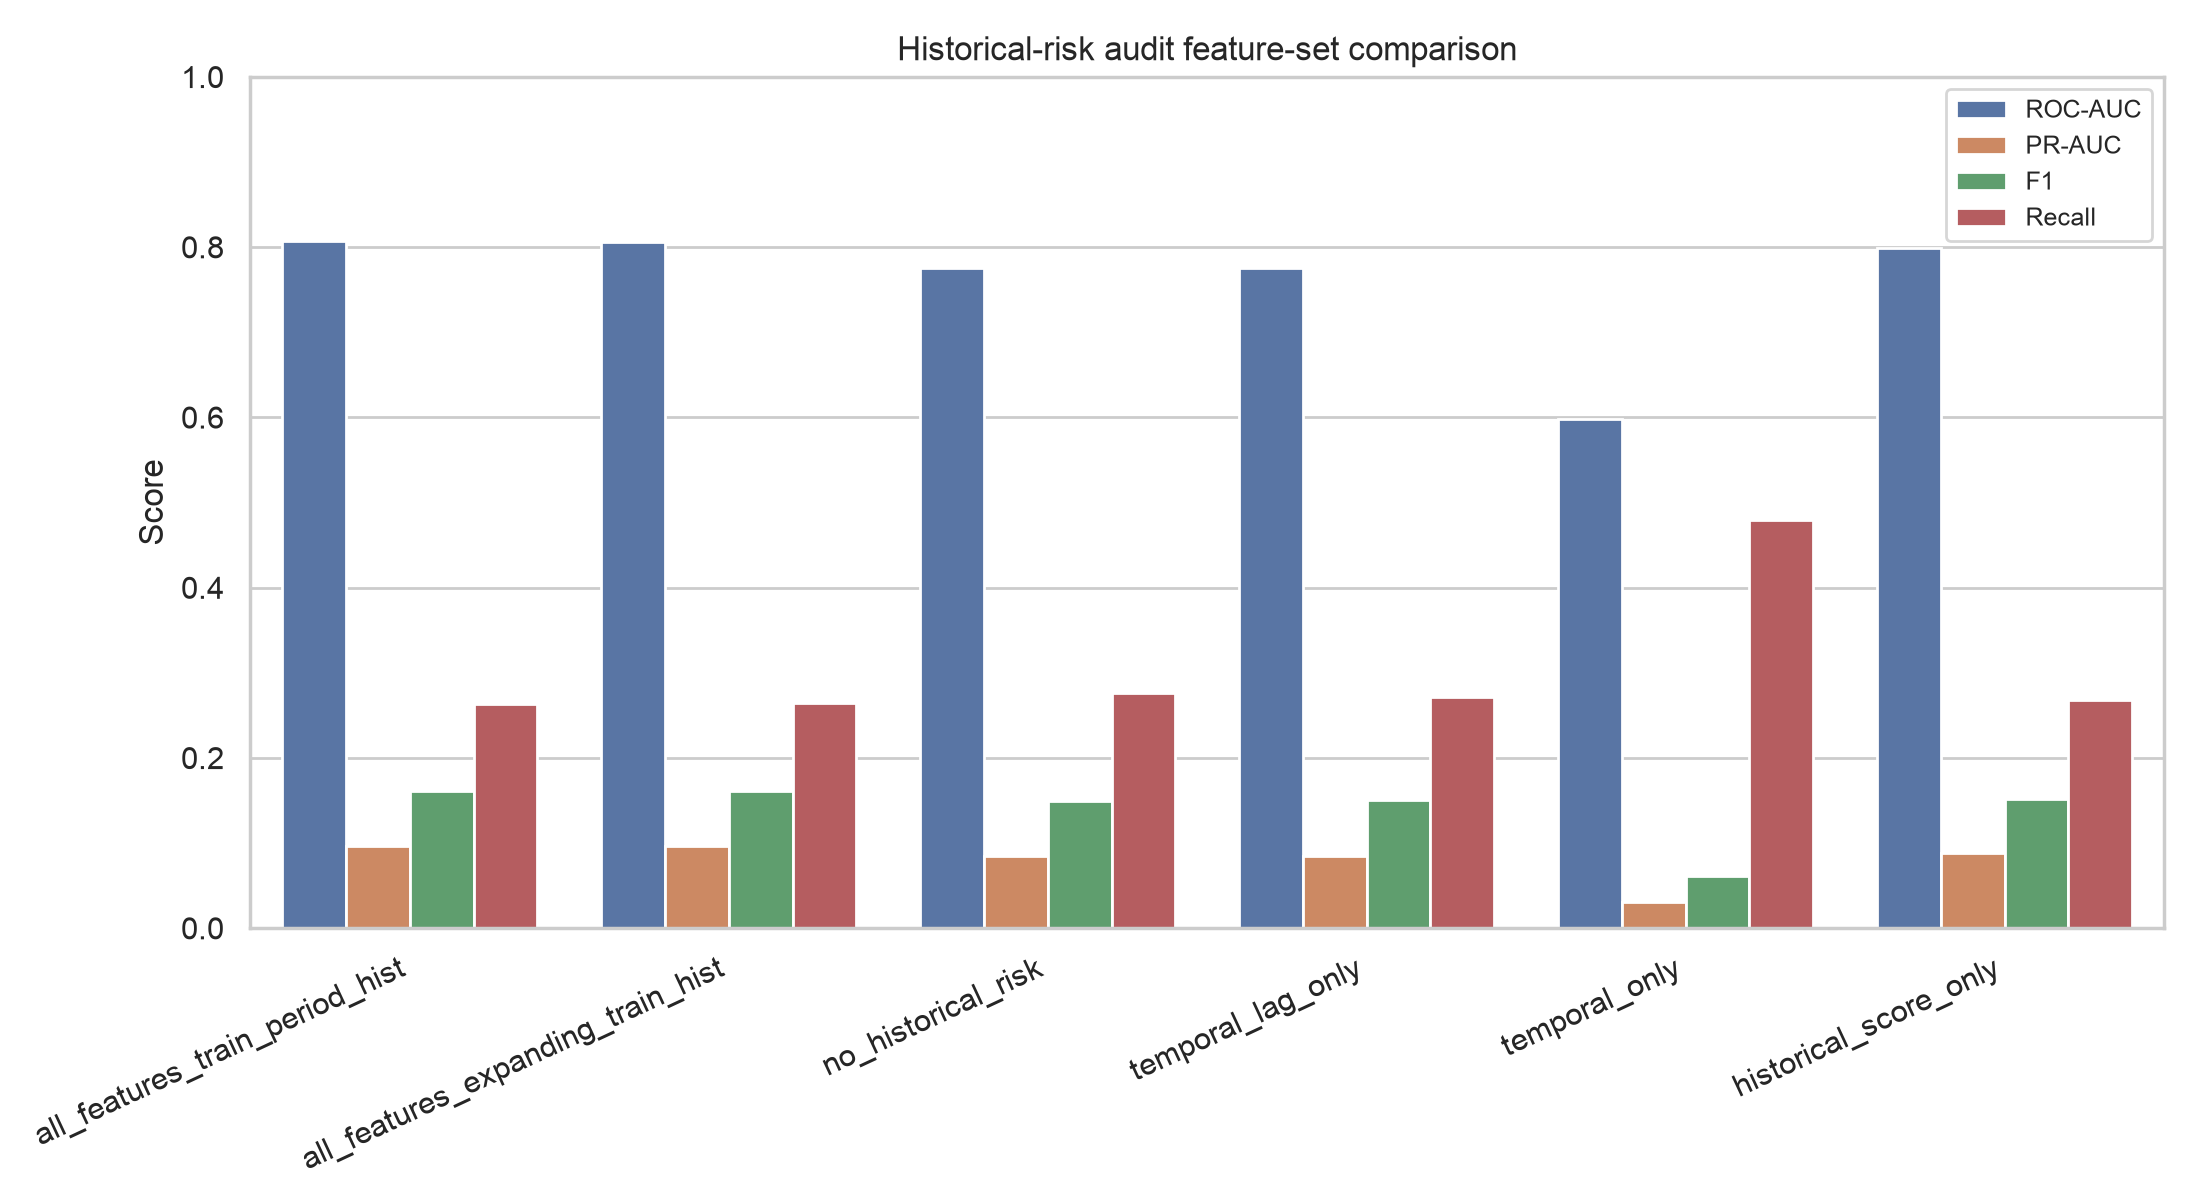
\includegraphics[width=0.88\textwidth]{historical_risk_audit_model_comparison.png}
\caption{Historical-risk feature audit result}
\label{fig:historical_risk_audit_model_comparison}
\end{figure}

\FloatBarrier

\section{H3 and time-window sensitivity checks}

Sensitivity checks compare the main H3 resolution-8, 3-hour setting with H3 resolution 7 and 9, and with 1-hour and 6-hour windows at resolution 8. The comparison uses historical risk and XGBoost with a controlled training design.

\begin{table}[H]
\centering
\caption{H3/time-window sensitivity result}
\label{tab:h3_time_sensitivity}
\small
\begin{tabular}{lrrrrr}
\toprule
\textbf{Setting} & \textbf{Cells} & \textbf{Window} & \textbf{Model} & \textbf{Test base rate} & \textbf{PR-AUC} \\
\midrule
H3-7 & 216 & 3h & XGBoost & 0.1309 & 0.2192 \\
H3-8 & 1,305 & 1h & XGBoost & 0.0084 & 0.0242 \\
H3-8 & 1,305 & 3h & XGBoost & 0.0242 & 0.0564 \\
H3-8 & 1,305 & 6h & XGBoost & 0.0465 & 0.0964 \\
H3-9 & 8,579 & 3h & XGBoost & 0.0038 & 0.0132 \\
\bottomrule
\end{tabular}
\end{table}

The sensitivity results must be read with the positive rate. H3-7 and 6-hour windows have higher PR-AUC partly because they are coarser and make positive labels less rare. H3-9 and 1-hour windows are much sparser. H3-8 with 3-hour windows remains the main setting because it balances spatial detail, temporal detail, dashboard usability, and computational cost. It is also the setting used for the full-grid model selection and final SHAP/LIME explanation.

The sensitivity check is therefore not a simple search for the largest PR-AUC. A coarser grid can look better because many incidents are merged into the same larger cell. A longer time window can look better because more incidents fall into each positive row. Those settings may be easier to predict but less useful for a map-based dashboard. H3-8 with 3-hour windows keeps a local spatial scale and a usable time scale while remaining computationally feasible.

\begin{figure}[H]
\centering
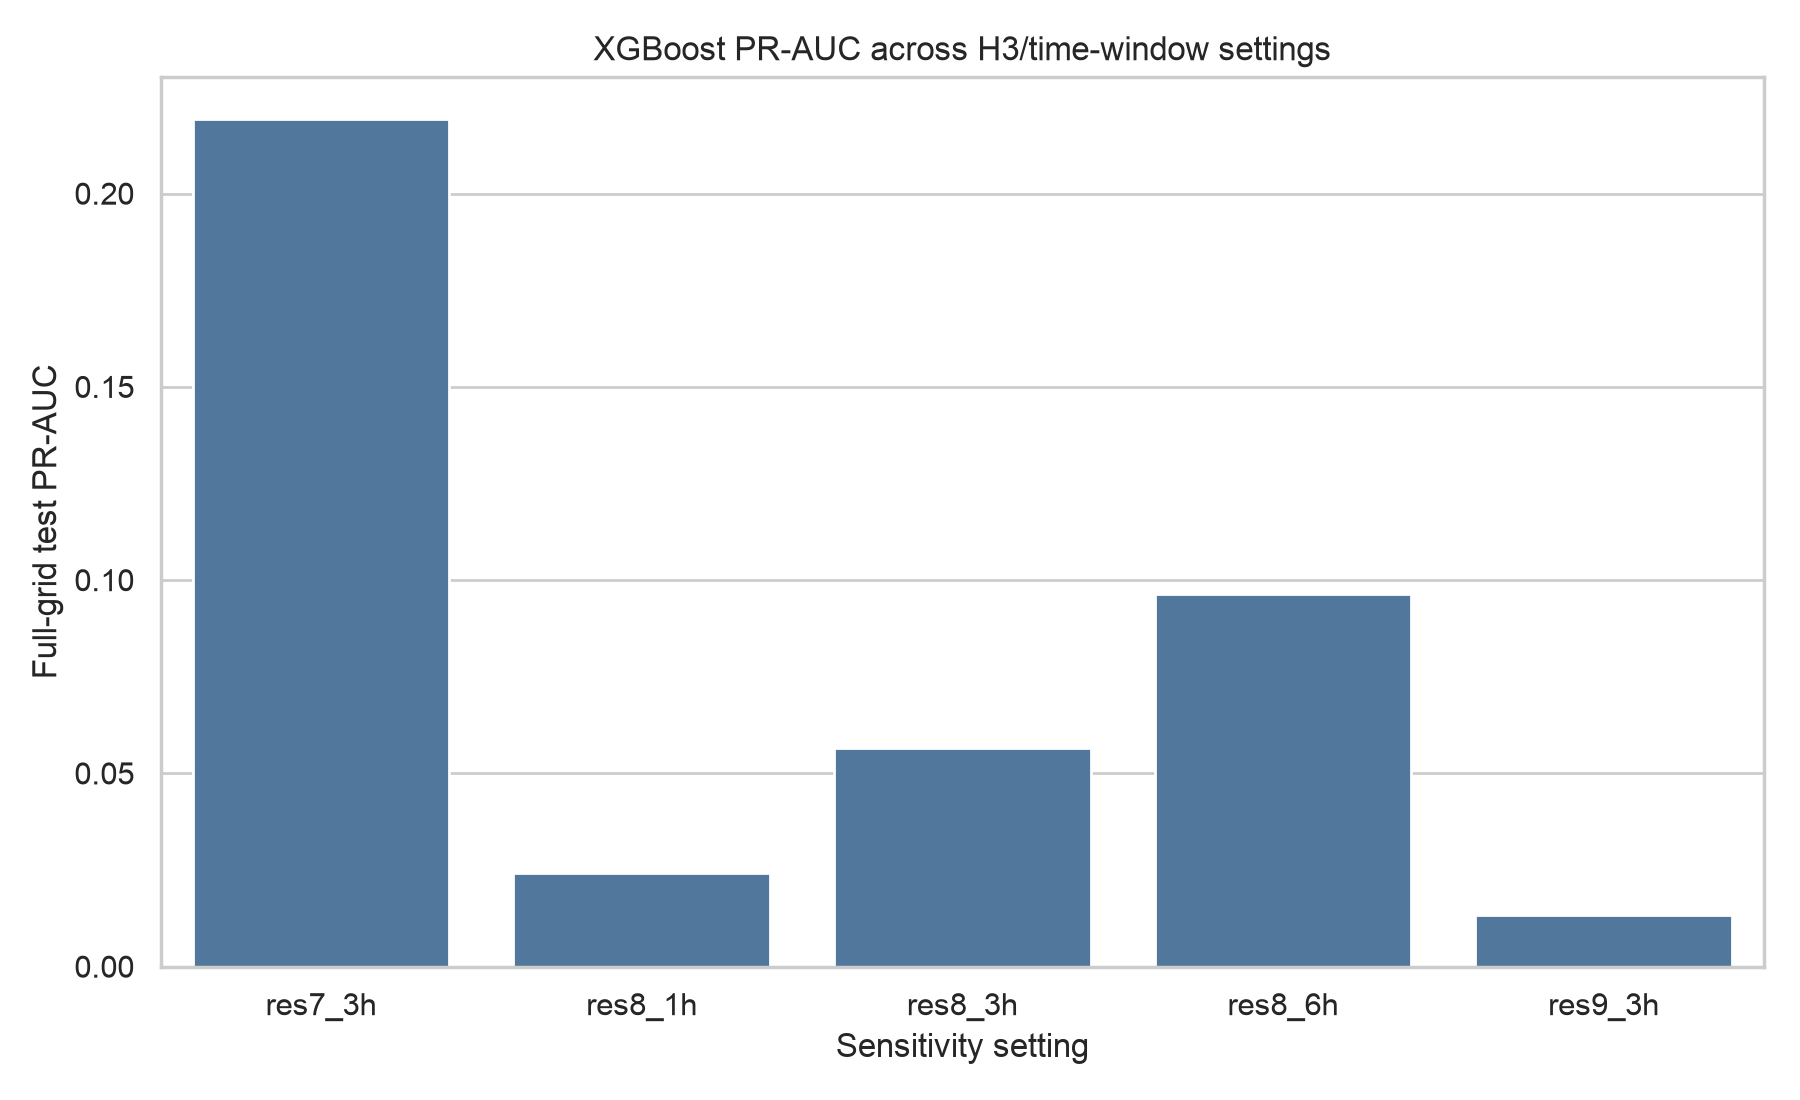
\includegraphics[width=0.88\textwidth]{h3_time_sensitivity_pr_auc.png}
\caption{H3/time-window sensitivity PR-AUC comparison}
\label{fig:h3_time_sensitivity_pr_auc}
\end{figure}

\begin{figure}[H]
\centering
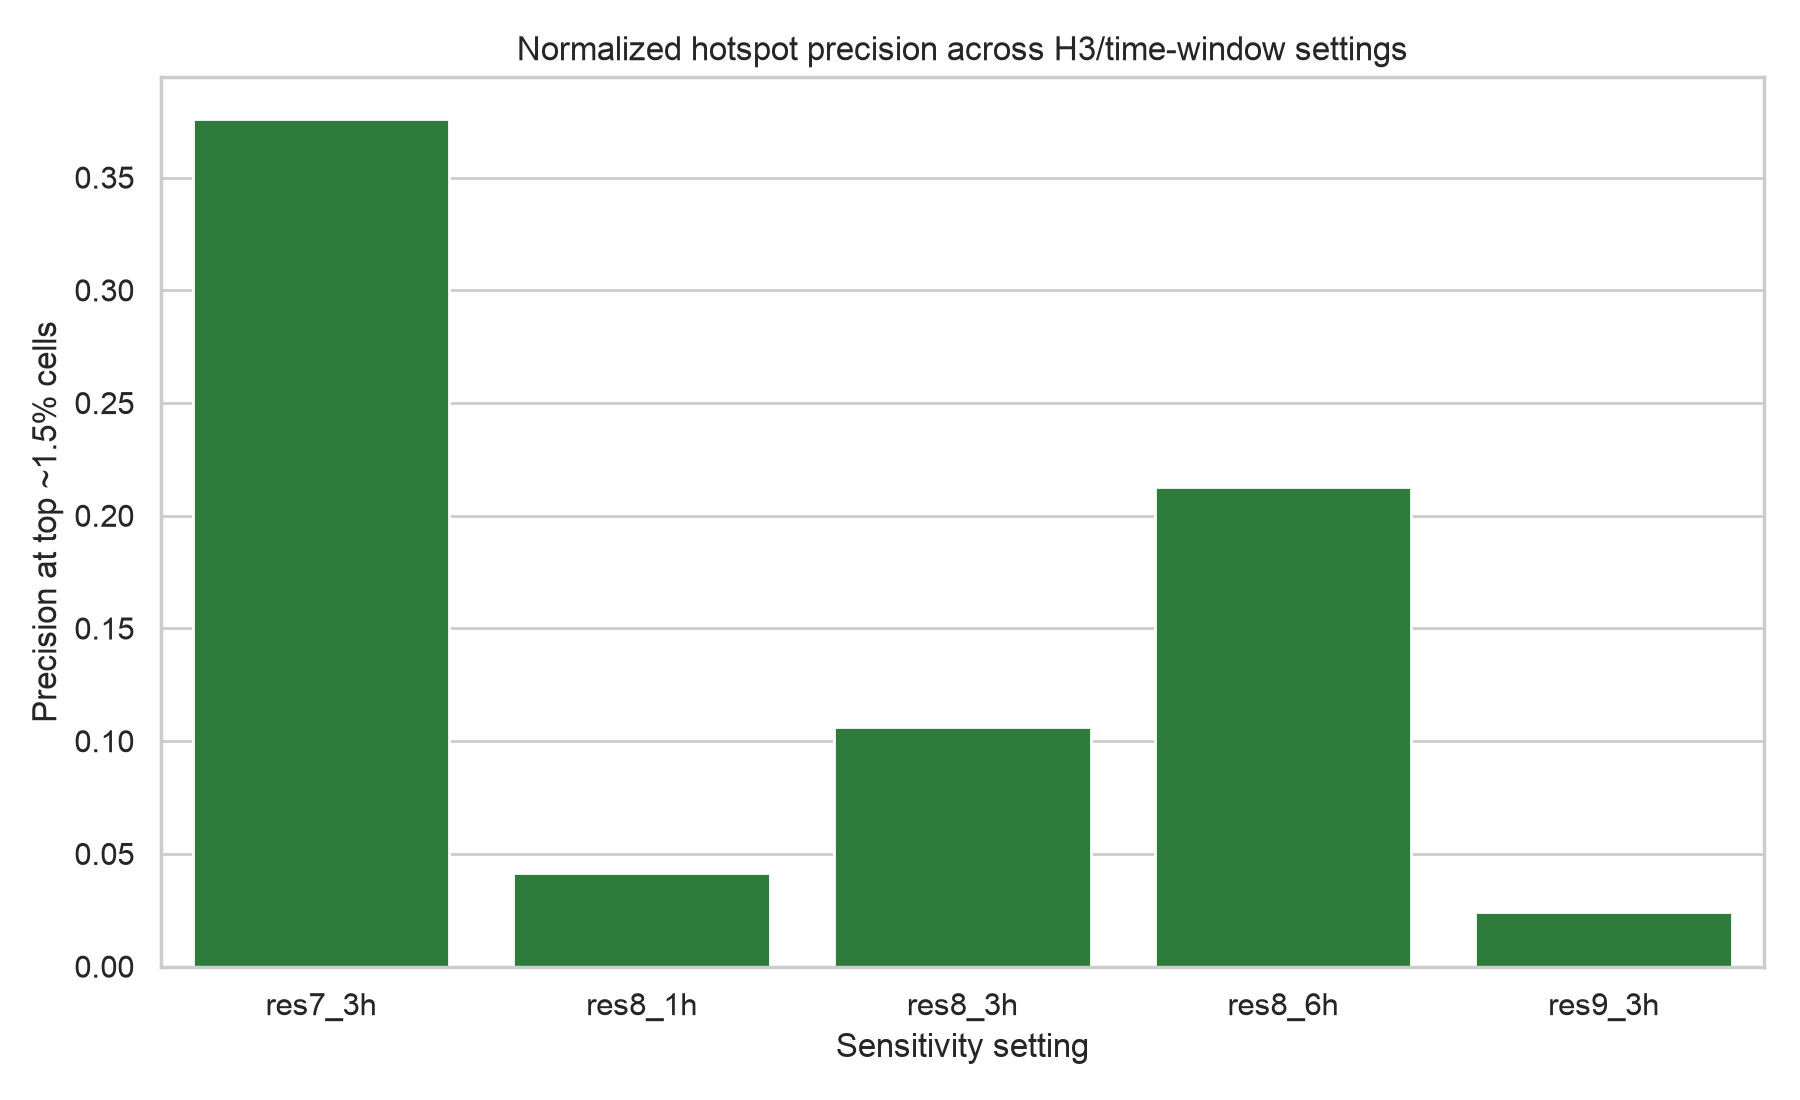
\includegraphics[width=0.88\textwidth]{h3_time_sensitivity_topk.png}
\caption{H3/time-window sensitivity top-k comparison.}
\label{fig:h3_time_sensitivity_topk_final}
\end{figure}

\begin{figure}[H]
\centering
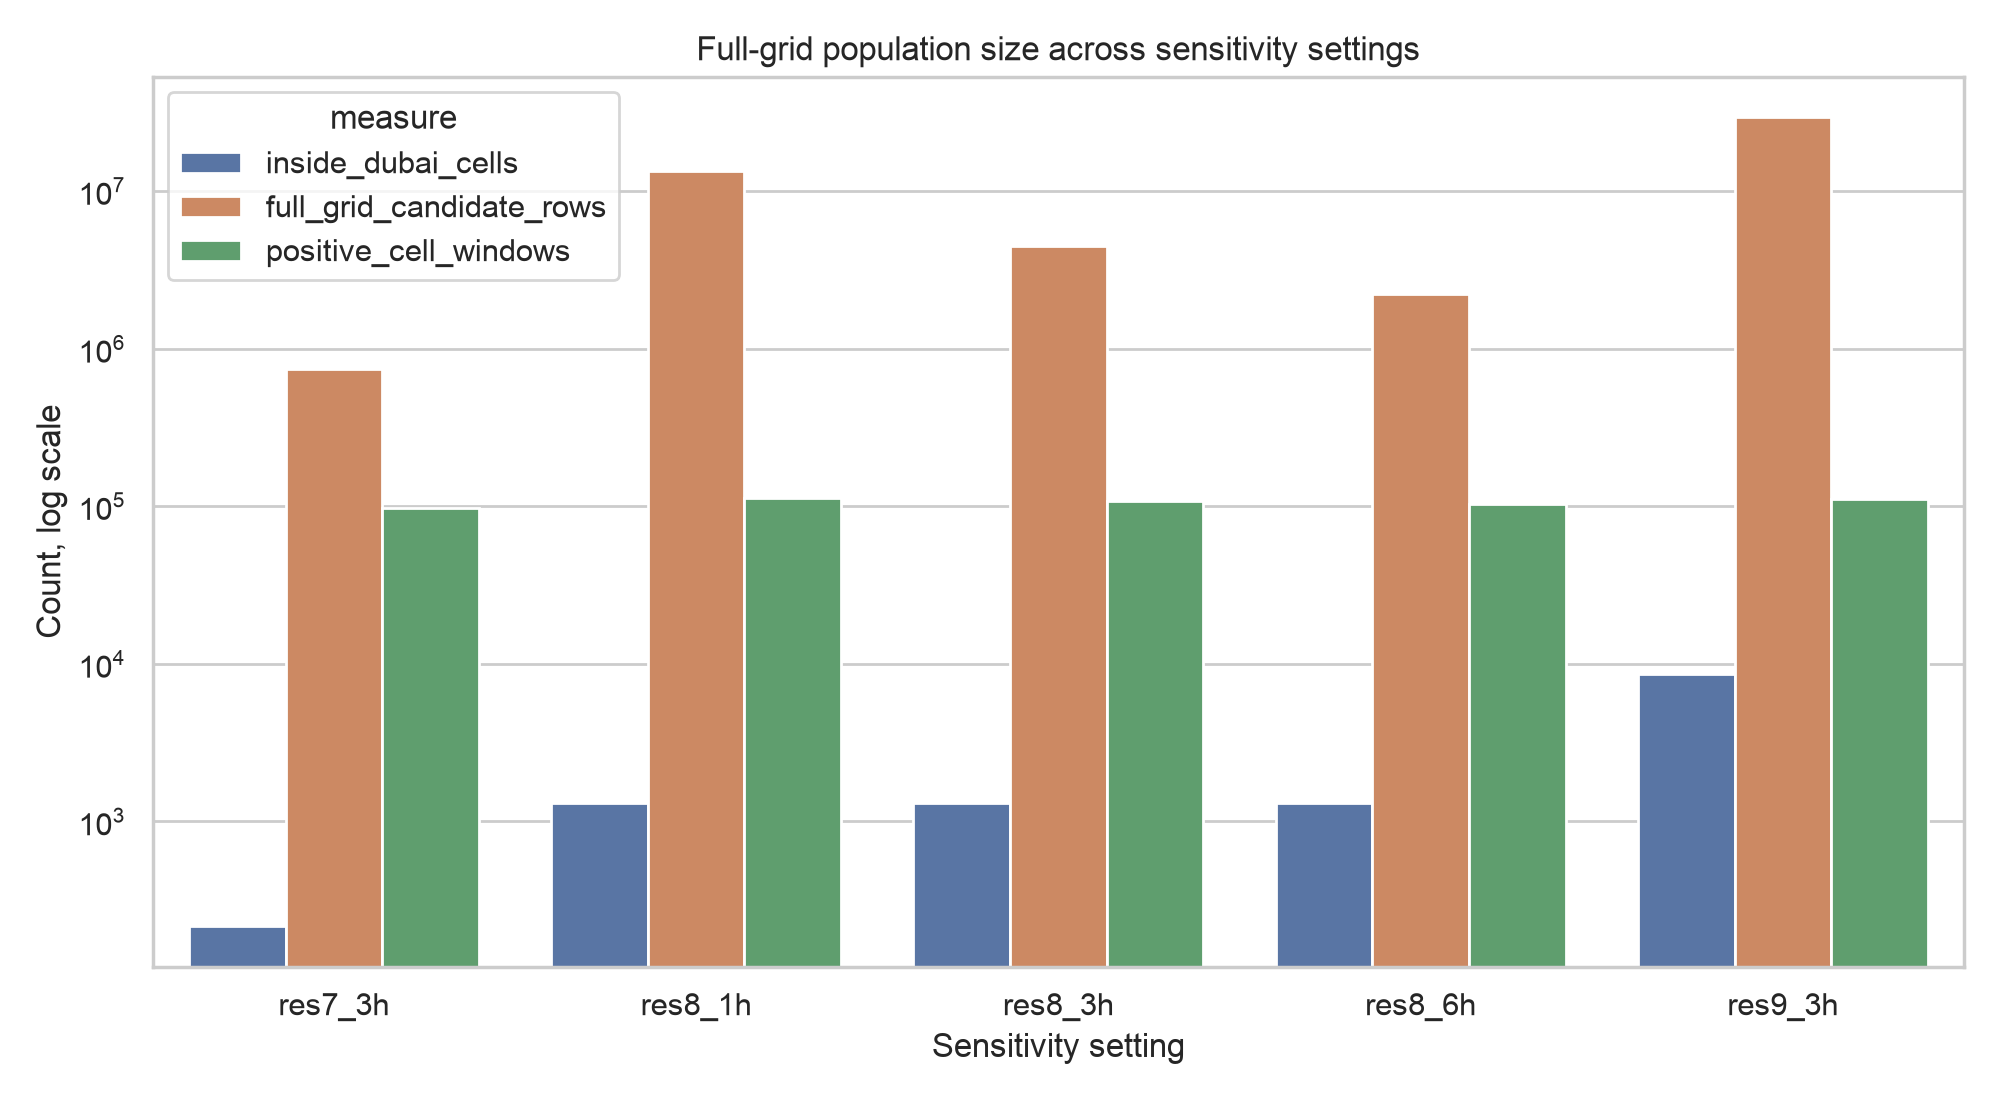
\includegraphics[width=0.88\textwidth]{h3_time_sensitivity_population.png}
\caption{H3/time-window sensitivity population comparison.}
\label{fig:h3_time_sensitivity_population_final}
\end{figure}

\FloatBarrier

\section{Neighboring-cell lag feature experiment}

A neighboring-cell feature experiment was added after the main full-grid evaluation. The purpose was to test whether recent incident activity in adjacent H3 cells improves prediction beyond the current same-cell temporal and historical-risk features. For each inside-Dubai H3 cell, ring-1 neighbors were obtained with \texttt{h3.grid\_disk(cell, 1)}. The center cell was excluded, and only inside-Dubai neighbors were retained. The inside-neighbor count ranges from 2 to 6, with a mean of 5.681.

The added features are previous 3-hour, 24-hour, and 7-day neighboring incident counts; previous 24-hour and 7-day neighboring severity-weighted sums; and previous 24-hour and 7-day neighboring active-cell counts. These features use only windows before the target prediction window. Unknown-severity incidents remain in incident counts, while unknown severity contributes zero to the severity-weighted sums.

\begin{table}[H]
\centering
\caption{Inside-Dubai full-grid result with neighboring H3 lag features}
\label{tab:neighbor_lag_feature_metrics}
\small
\begin{tabular}{lrrrrr}
\toprule
\textbf{Model} & \textbf{ROC-AUC} & \textbf{PR-AUC} & \textbf{Precision} & \textbf{Recall} & \textbf{F1} \\
\midrule
Historical risk & 0.7990 & 0.0882 & 0.1063 & 0.2679 & 0.1522 \\
XGBoost current features & 0.8067 & 0.0967 & 0.1165 & 0.2630 & 0.1615 \\
XGBoost + neighbor lags & 0.8120 & 0.0992 & 0.1179 & 0.2720 & 0.1645 \\
\bottomrule
\end{tabular}
\end{table}

The neighboring-cell lag features give a modest but consistent improvement. PR-AUC increases by 0.0025, ROC-AUC increases by 0.0053, and F1-score increases by 0.0030 compared with the current XGBoost feature set. This suggests that nearby recent activity contains additional spatial signal, but the improvement is not large enough to change the interpretation that historical cell/time risk remains the dominant predictor.

This result is useful because it improves the model without changing the thesis formulation. The target remains binary incident occurrence. The spatial unit remains H3 resolution 8. The validation and test periods remain full-grid and untouched. Only the feature set changes by adding information from adjacent cells in previous windows. Since the improvement is consistent across PR-AUC, F1, and top-k capture, the neighbor features are promoted into the final model path.

\begin{table}[H]
\centering
\caption{Top-k hotspot ranking with neighboring H3 lag features}
\label{tab:neighbor_lag_feature_topk}
\small
\begin{tabular}{lrrrr}
\toprule
\textbf{Model} & \textbf{k} & \textbf{Recall@k} & \textbf{Precision@k} & \textbf{Incident recall@k} \\
\midrule
Historical risk & 20 & 0.0817 & 0.1293 & 0.0871 \\
XGBoost current features & 20 & 0.0836 & 0.1323 & 0.0892 \\
XGBoost + neighbor lags & 20 & 0.0844 & 0.1336 & 0.0903 \\
\bottomrule
\end{tabular}
\end{table}

At top 20, the neighbor-feature model captures 9,138 positive cell/windows and 10,416 incidents, compared with 9,049 positive cell/windows and 10,281 incidents for the current XGBoost model. The gain is small, but it supports keeping neighboring-cell lag features as part of the final model-improvement path before tuning and calibration.

\begin{figure}[H]
\centering
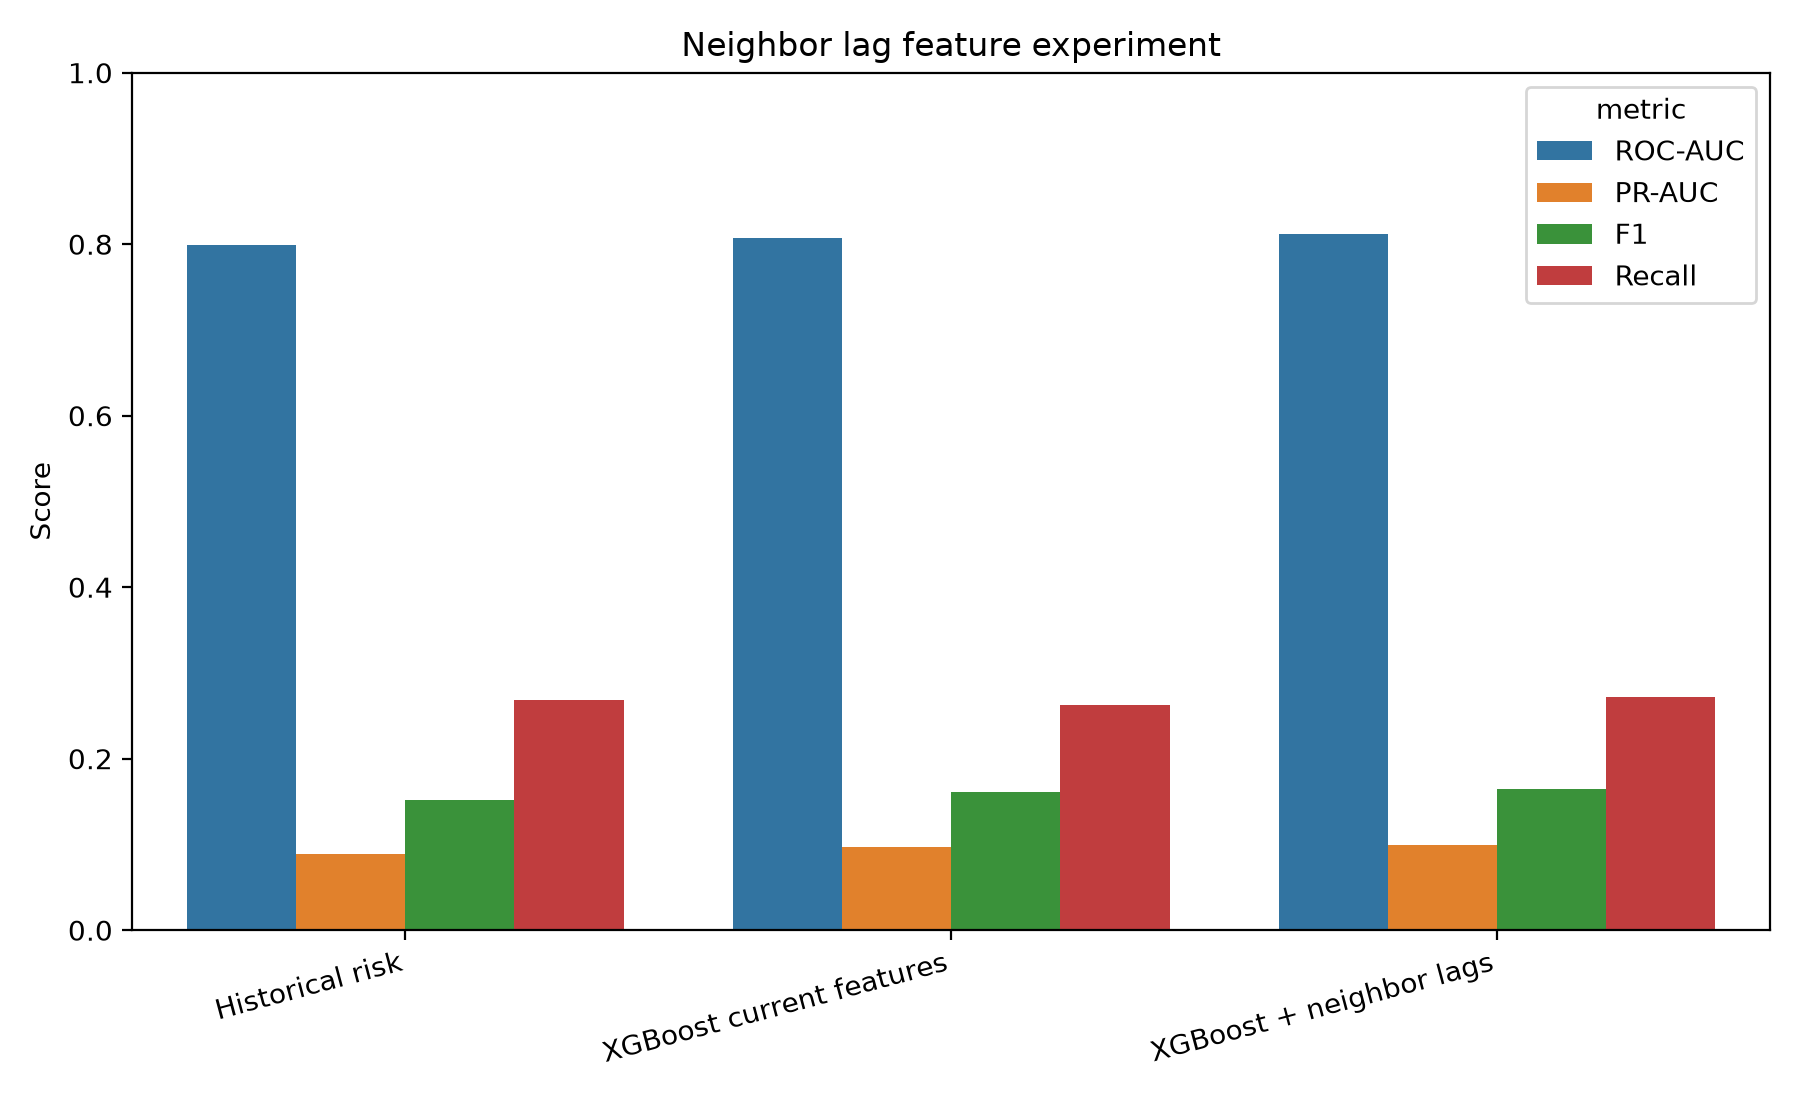
\includegraphics[width=0.88\textwidth]{neighbor_lag_feature_model_comparison.png}
\caption{Neighboring H3 lag feature model comparison}
\label{fig:neighbor_lag_feature_model_comparison}
\end{figure}

\begin{figure}[H]
\centering
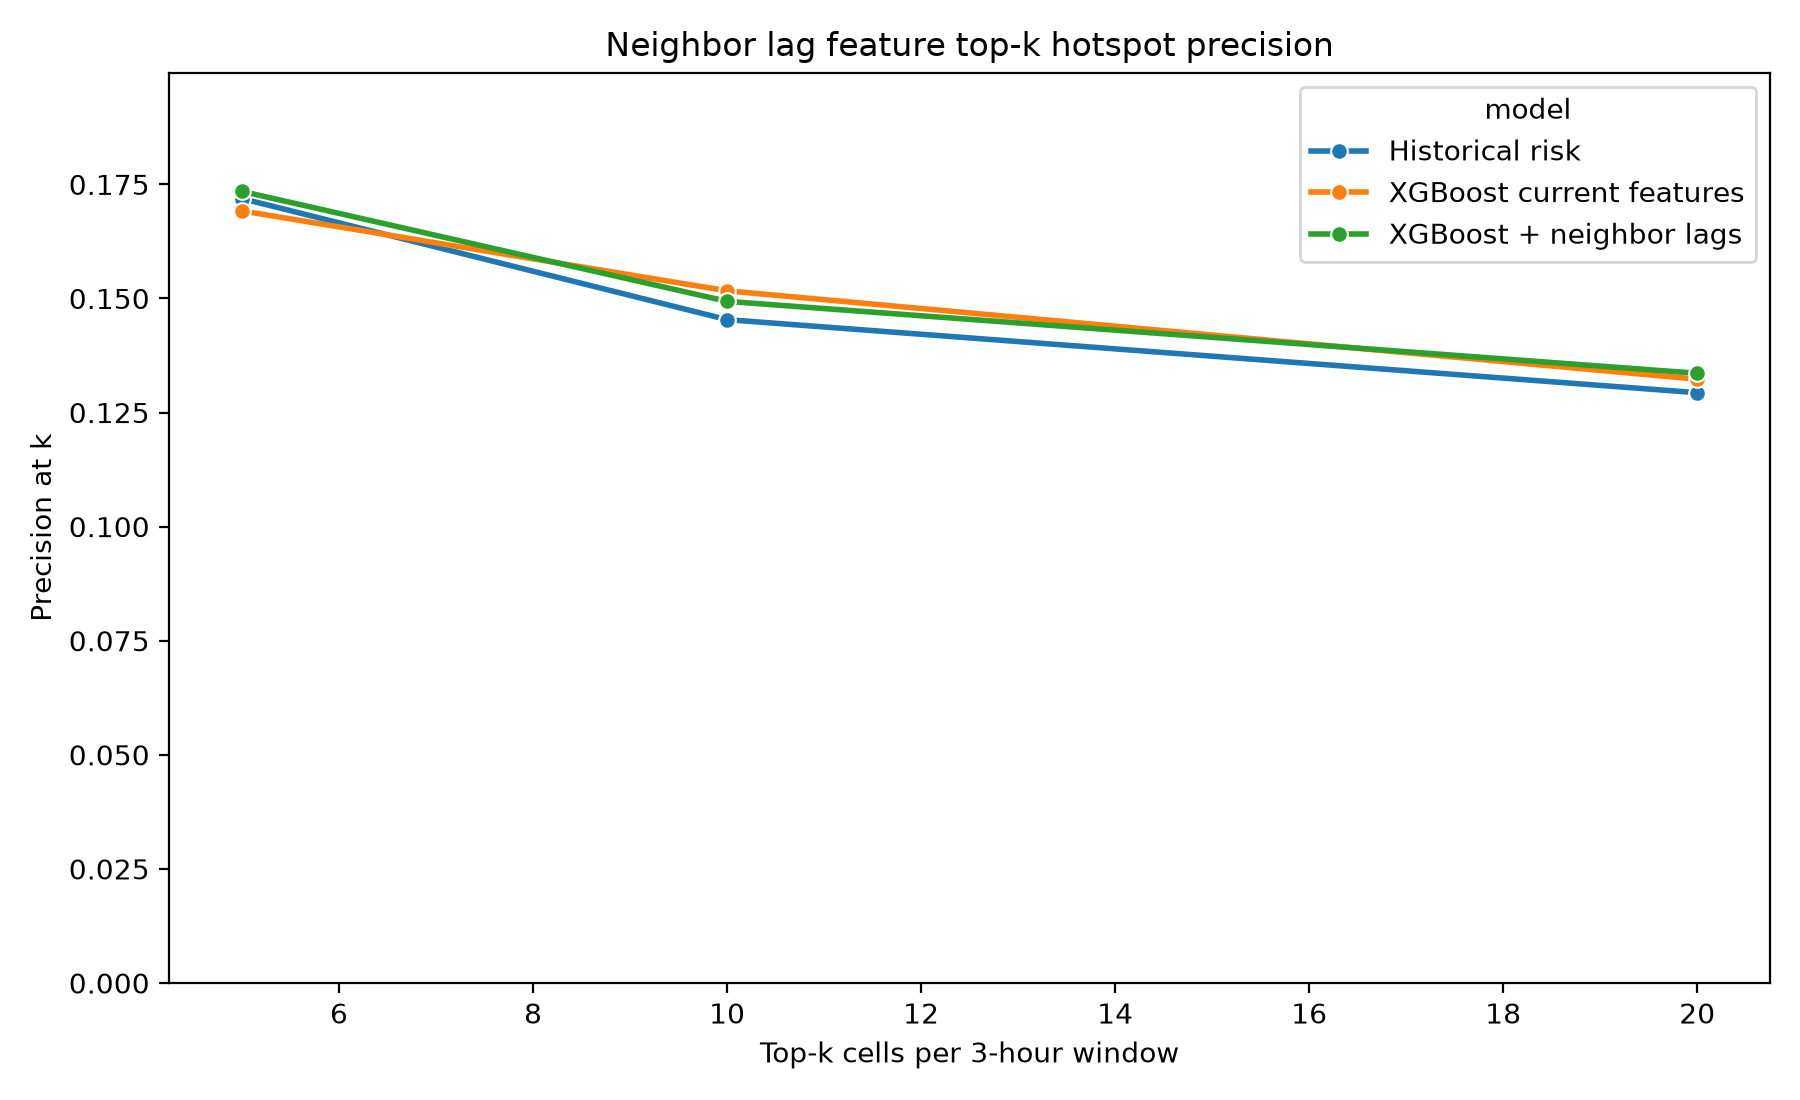
\includegraphics[width=0.88\textwidth]{neighbor_lag_feature_topk_comparison.png}
\caption{Neighboring H3 lag feature top-k comparison}
\label{fig:neighbor_lag_feature_topk_comparison}
\end{figure}

\FloatBarrier

\section{Hard-negative training sample experiment}

After the neighboring-cell feature experiment, a hard-negative training sample was tested. The aim was to see whether the XGBoost model would improve if it learned from training-window cell/time pairs that looked risky to the current model but did not contain incidents. A deterministic miner model was first trained with the existing random-negative training sample. It then scored all full-grid training negatives. The final hard-negative sample kept all positive training rows and filled the remaining training budget with 70\% high-scoring hard negatives and 30\% random negatives. Validation and test remained full-grid and unchanged.

\begin{table}[H]
\centering
\caption{Hard-negative and random-negative training sample composition}
\label{tab:hard_negative_training_sample}
\footnotesize
\begin{tabular}{lrrrrr}
\toprule
\textbf{Sample} & \textbf{Rows} & \textbf{Pos.} & \textbf{Neg.} & \textbf{Hard neg.} & \textbf{Rand. neg.} \\
\midrule
Current random sample & 1,000,000 & 296,022 & 703,978 & 0 & 703,978 \\
Hard-negative sample & 1,000,000 & 360,278 & 639,722 & 447,805 & 191,917 \\
\bottomrule
\end{tabular}
\end{table}

\begin{table}[H]
\centering
\caption{Inside-Dubai full-grid result with hard-negative training}
\label{tab:hard_negative_training_metrics}
\footnotesize
\begin{tabularx}{\textwidth}{L{0.34\textwidth}rrrrr}
\toprule
\textbf{Model} & \textbf{ROC-AUC} & \textbf{PR-AUC} & \textbf{Precision} & \textbf{Recall} & \textbf{F1} \\
\midrule
Historical risk & 0.7990 & 0.0882 & 0.1063 & 0.2679 & 0.1522 \\
XGBoost neighbor random sample & 0.8120 & 0.0992 & 0.1179 & 0.2720 & 0.1645 \\
XGBoost neighbor hard negatives & 0.6934 & 0.0487 & 0.0599 & 0.3333 & 0.1015 \\
\bottomrule
\end{tabularx}
\end{table}

The hard-negative sample did not improve the model. PR-AUC fell from 0.0992 to 0.0487, F1 fell from 0.1645 to 0.1015, and precision fell from 0.1179 to 0.0599. Recall increased, but the increase came with many more false positives. This is not a useful tradeoff for hotspot ranking.

This failed experiment is still important. It shows that the thesis did not simply accept every added technique. Hard-negative mining is plausible for rare-event prediction because it gives the model difficult negative examples. In this dataset, however, the tested 70/30 hard-negative strategy appears too aggressive. It teaches the model that many historically risky-looking rows are negative, which reduces the model's ability to rank true future hotspots.

\begin{table}[H]
\centering
\caption{Top-k hotspot ranking with hard-negative training}
\label{tab:hard_negative_training_topk}
\small
\begin{tabular}{lrrrr}
\toprule
\textbf{Model} & \textbf{k} & \textbf{Recall@k} & \textbf{Precision@k} & \textbf{Incident recall@k} \\
\midrule
Historical risk & 20 & 0.0817 & 0.1293 & 0.0871 \\
XGBoost neighbor random sample & 20 & 0.0844 & 0.1336 & 0.0903 \\
XGBoost neighbor hard negatives & 20 & 0.0386 & 0.0610 & 0.0384 \\
\bottomrule
\end{tabular}
\end{table}

At top 20, the hard-negative model captures 4,427 incidents, compared with 10,416 for the random-sample neighbor-feature model. The likely reason is that the hard-negative sample over-emphasizes difficult high-risk-looking non-incident rows. That teaches the model to suppress scores in historically risky areas, which damages the ranking of true hotspots in the later test period. For the current thesis pipeline, the hard-negative strategy is therefore rejected.

\begin{figure}[H]
\centering
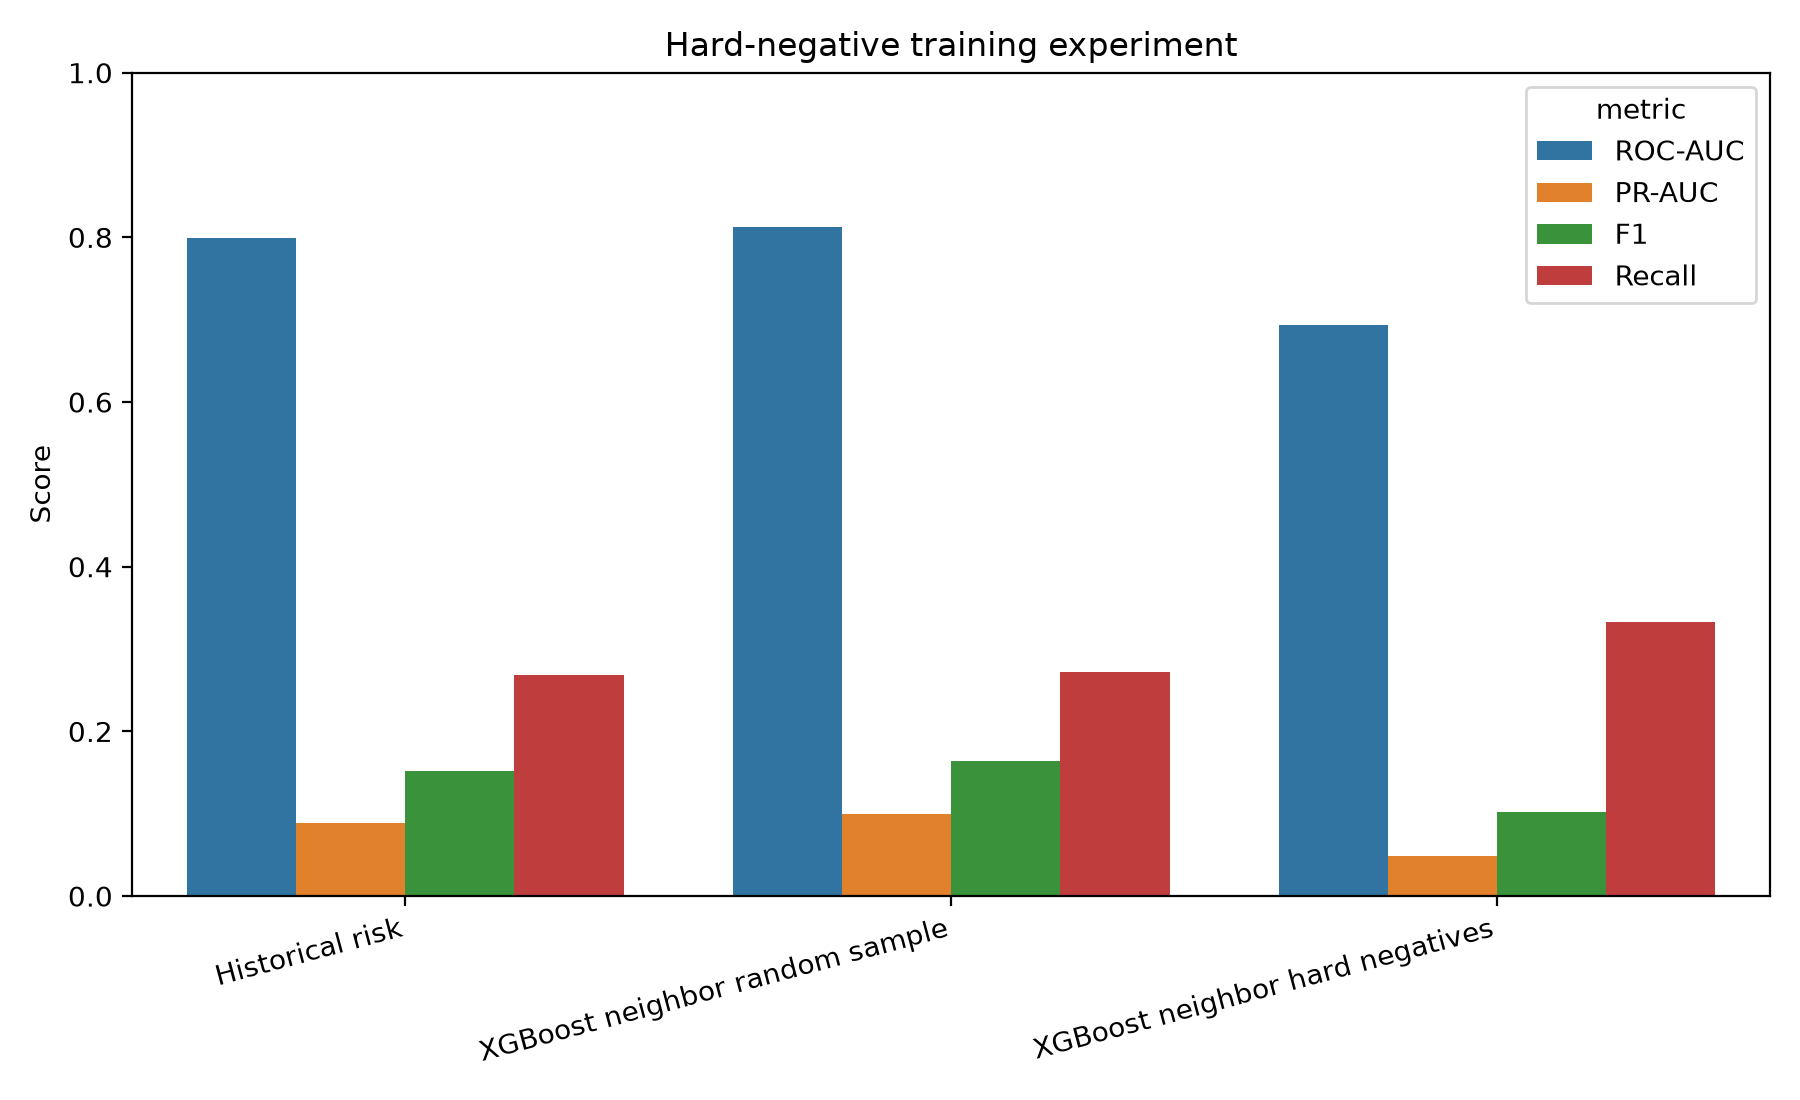
\includegraphics[width=0.88\textwidth]{hard_negative_training_model_comparison.png}
\caption{Hard-negative training model comparison}
\label{fig:hard_negative_training_model_comparison}
\end{figure}

\begin{figure}[H]
\centering
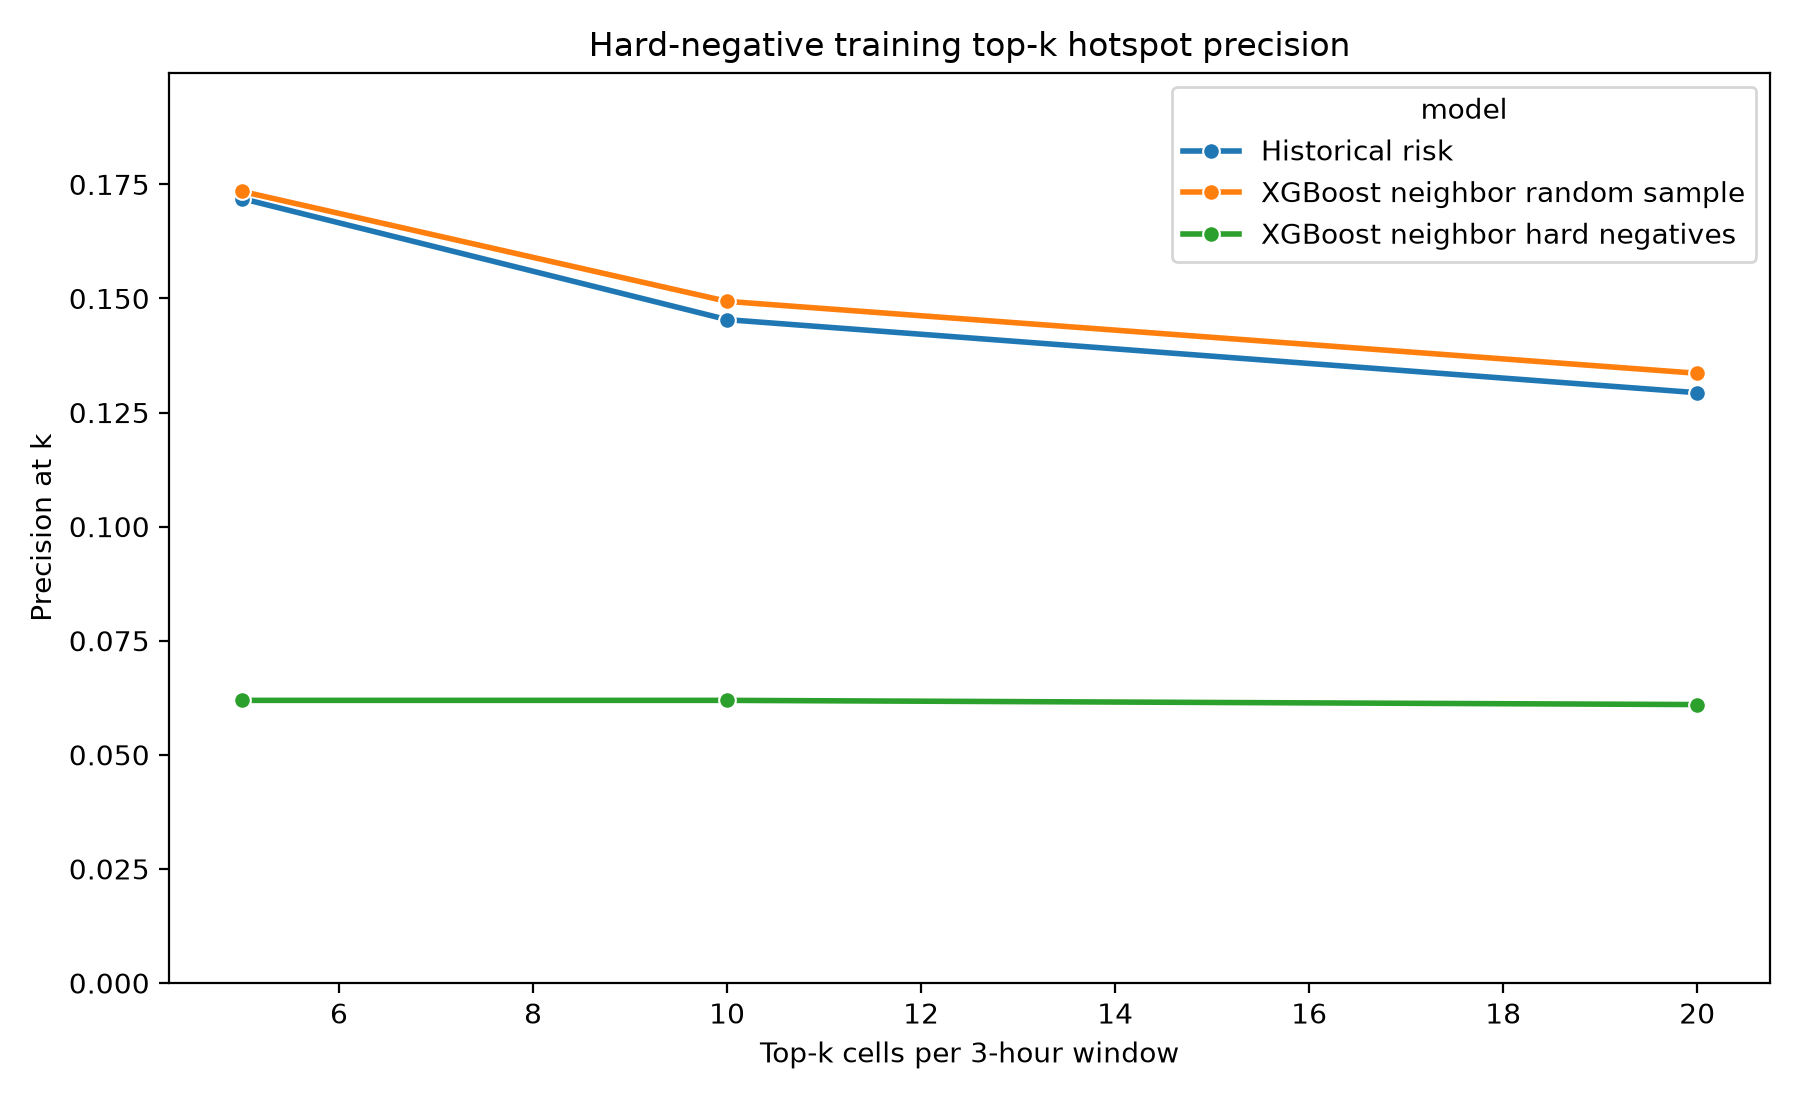
\includegraphics[width=0.88\textwidth]{hard_negative_training_topk_comparison.png}
\caption{Hard-negative training top-k comparison}
\label{fig:hard_negative_training_topk_comparison}
\end{figure}

\FloatBarrier

\section{XGBoost hyperparameter tuning experiment}

After rejecting the hard-negative training sample, XGBoost hyperparameters were tuned for the neighbor-feature model while keeping the original sampled-negative training table. The search used 18 predeclared candidates over tree depth, learning rate, number of estimators, and minimum child weight. All candidates used the same training rows and the same neighbor-lag features. The selection rule used validation data only: highest validation PR-AUC, then validation top-20 incident recall for candidates within 0.001 PR-AUC, then validation F1.

The selected candidate was \texttt{xgb\_tune\_12}, with maximum depth 5, learning rate 0.10, 240 estimators, and minimum child weight 10. It was selected because it was within 0.001 validation PR-AUC of the best candidate and had the strongest validation top-20 incident recall among that group.

\begin{table}[H]
\centering
\caption{Selected XGBoost tuning configuration}
\label{tab:xgboost_tuning_selected_config}
\small
\begin{tabular}{lrrrr}
\toprule
\textbf{Candidate} & \textbf{Depth} & \textbf{Learning rate} & \textbf{Estimators} & \textbf{Min child weight} \\
\midrule
\texttt{xgb\_tune\_12} & 5 & 0.10 & 240 & 10 \\
\bottomrule
\end{tabular}
\end{table}

\begin{table}[H]
\centering
\caption{Inside-Dubai full-grid result after XGBoost tuning}
\label{tab:xgboost_tuning_test_metrics}
\small
\begin{tabular}{lrrrrr}
\toprule
\textbf{Model} & \textbf{ROC-AUC} & \textbf{PR-AUC} & \textbf{Precision} & \textbf{Recall} & \textbf{F1} \\
\midrule
Historical risk & 0.7990 & 0.0882 & 0.1063 & 0.2679 & 0.1522 \\
XGBoost neighbor default & 0.8120 & 0.0992 & 0.1179 & 0.2720 & 0.1645 \\
XGBoost neighbor tuned & 0.8088 & 0.0976 & 0.1156 & 0.2710 & 0.1620 \\
\bottomrule
\end{tabular}
\end{table}

The tuned model did not improve the untouched test result. Test PR-AUC fell from 0.0992 to 0.0976 and F1 fell from 0.1645 to 0.1620. The difference is small, but it does not justify replacing the default neighbor-feature XGBoost model.

The tuning result is a useful caution. The selected candidate was chosen using validation data only, so the procedure itself is valid. The untouched test result shows that the selected candidate does not generalize better than the default neighbor-feature model. This is why the final model is not the most complex or most tuned version. The report keeps the simpler default configuration because it performs slightly better on the final test period and is easier to defend.

\begin{table}[H]
\centering
\caption{Top-k hotspot ranking after XGBoost tuning}
\label{tab:xgboost_tuning_topk}
\small
\begin{tabular}{lrrrr}
\toprule
\textbf{Model} & \textbf{k} & \textbf{Recall@k} & \textbf{Precision@k} & \textbf{Incident recall@k} \\
\midrule
Historical risk & 20 & 0.0817 & 0.1293 & 0.0871 \\
XGBoost neighbor default & 20 & 0.0844 & 0.1336 & 0.0903 \\
XGBoost neighbor tuned & 20 & 0.0838 & 0.1327 & 0.0895 \\
\bottomrule
\end{tabular}
\end{table}

At top 20, the tuned model captures 10,323 incidents, compared with 10,416 for the default neighbor-feature XGBoost. The default model therefore remains the current final candidate for the calibration and dashboard stages.

\begin{figure}[H]
\centering
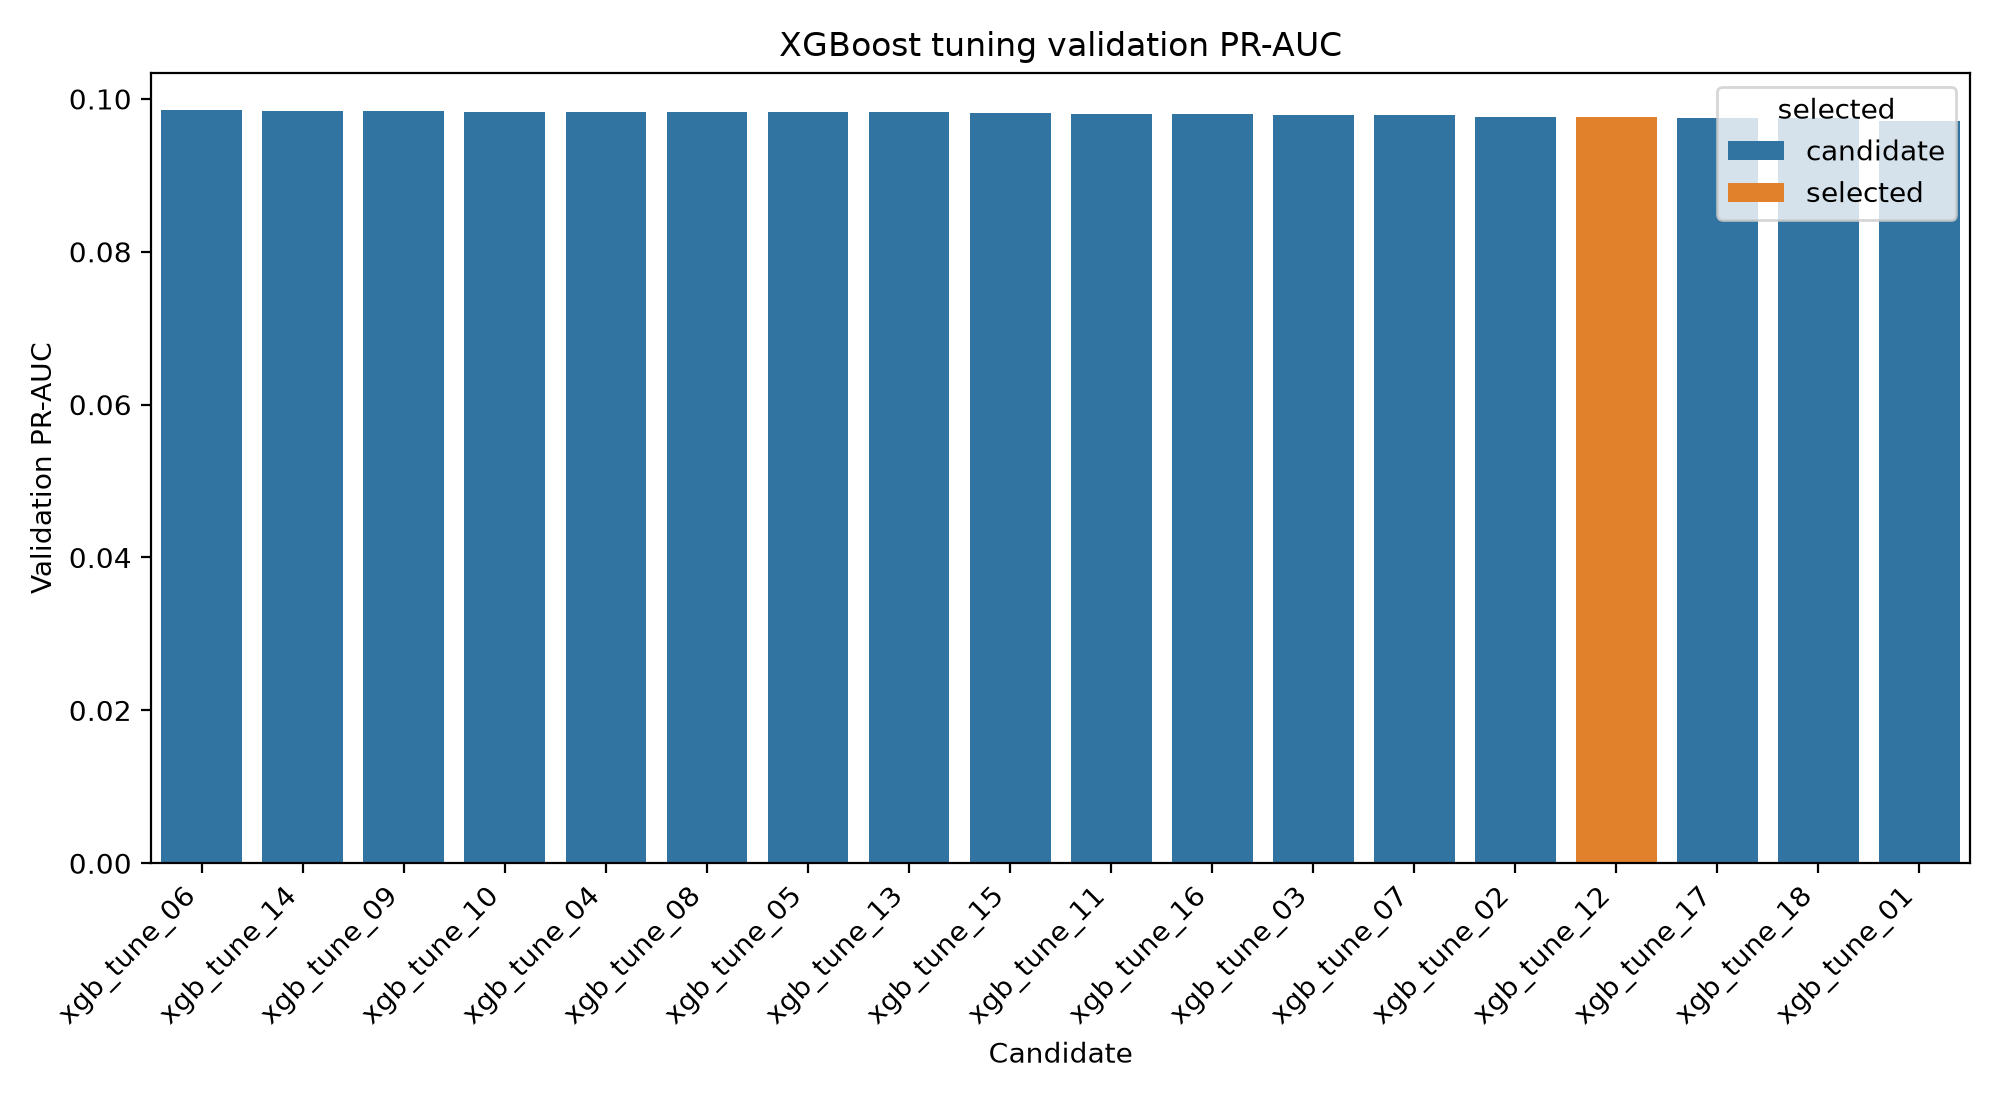
\includegraphics[width=0.88\textwidth]{xgboost_tuning_validation_pr_auc.png}
\caption{XGBoost tuning validation PR-AUC by candidate}
\label{fig:xgboost_tuning_validation_pr_auc}
\end{figure}

\begin{figure}[H]
\centering
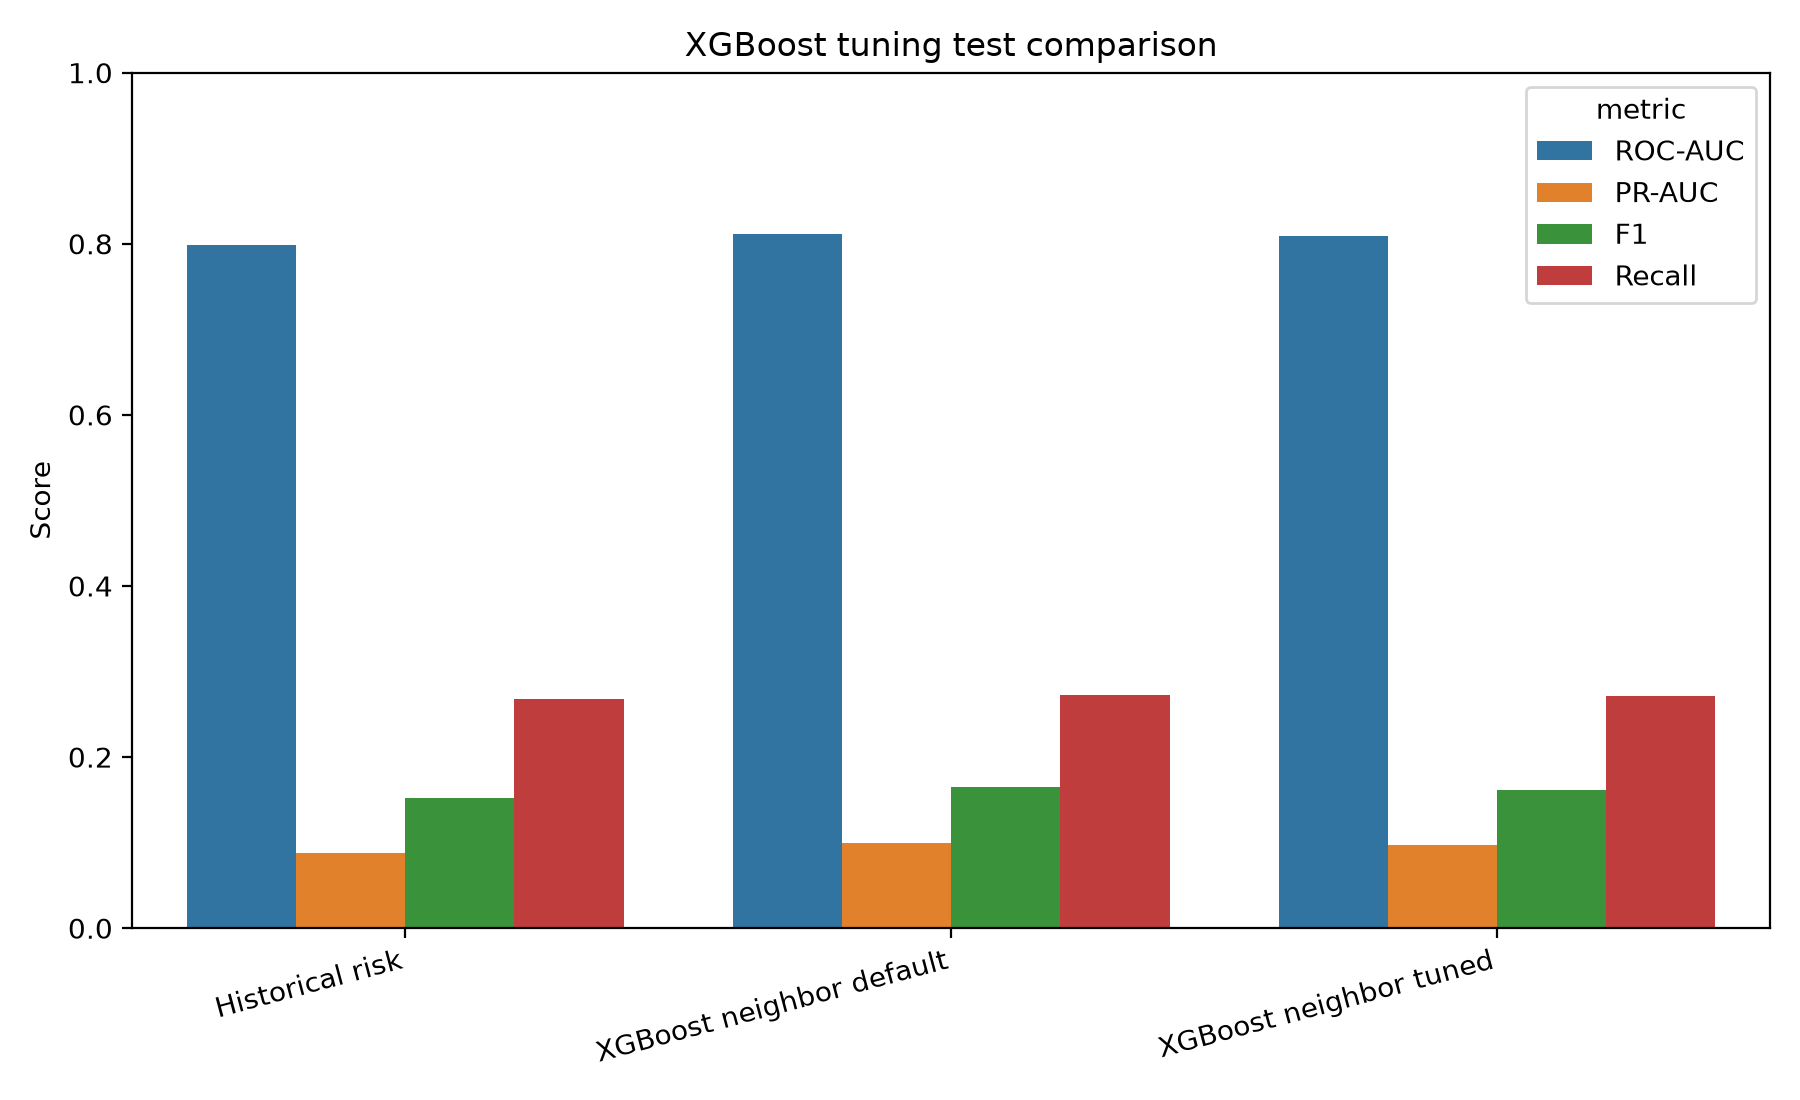
\includegraphics[width=0.88\textwidth]{xgboost_tuning_test_comparison.png}
\caption{XGBoost tuning test comparison}
\label{fig:xgboost_tuning_test_comparison}
\end{figure}

\begin{figure}[H]
\centering
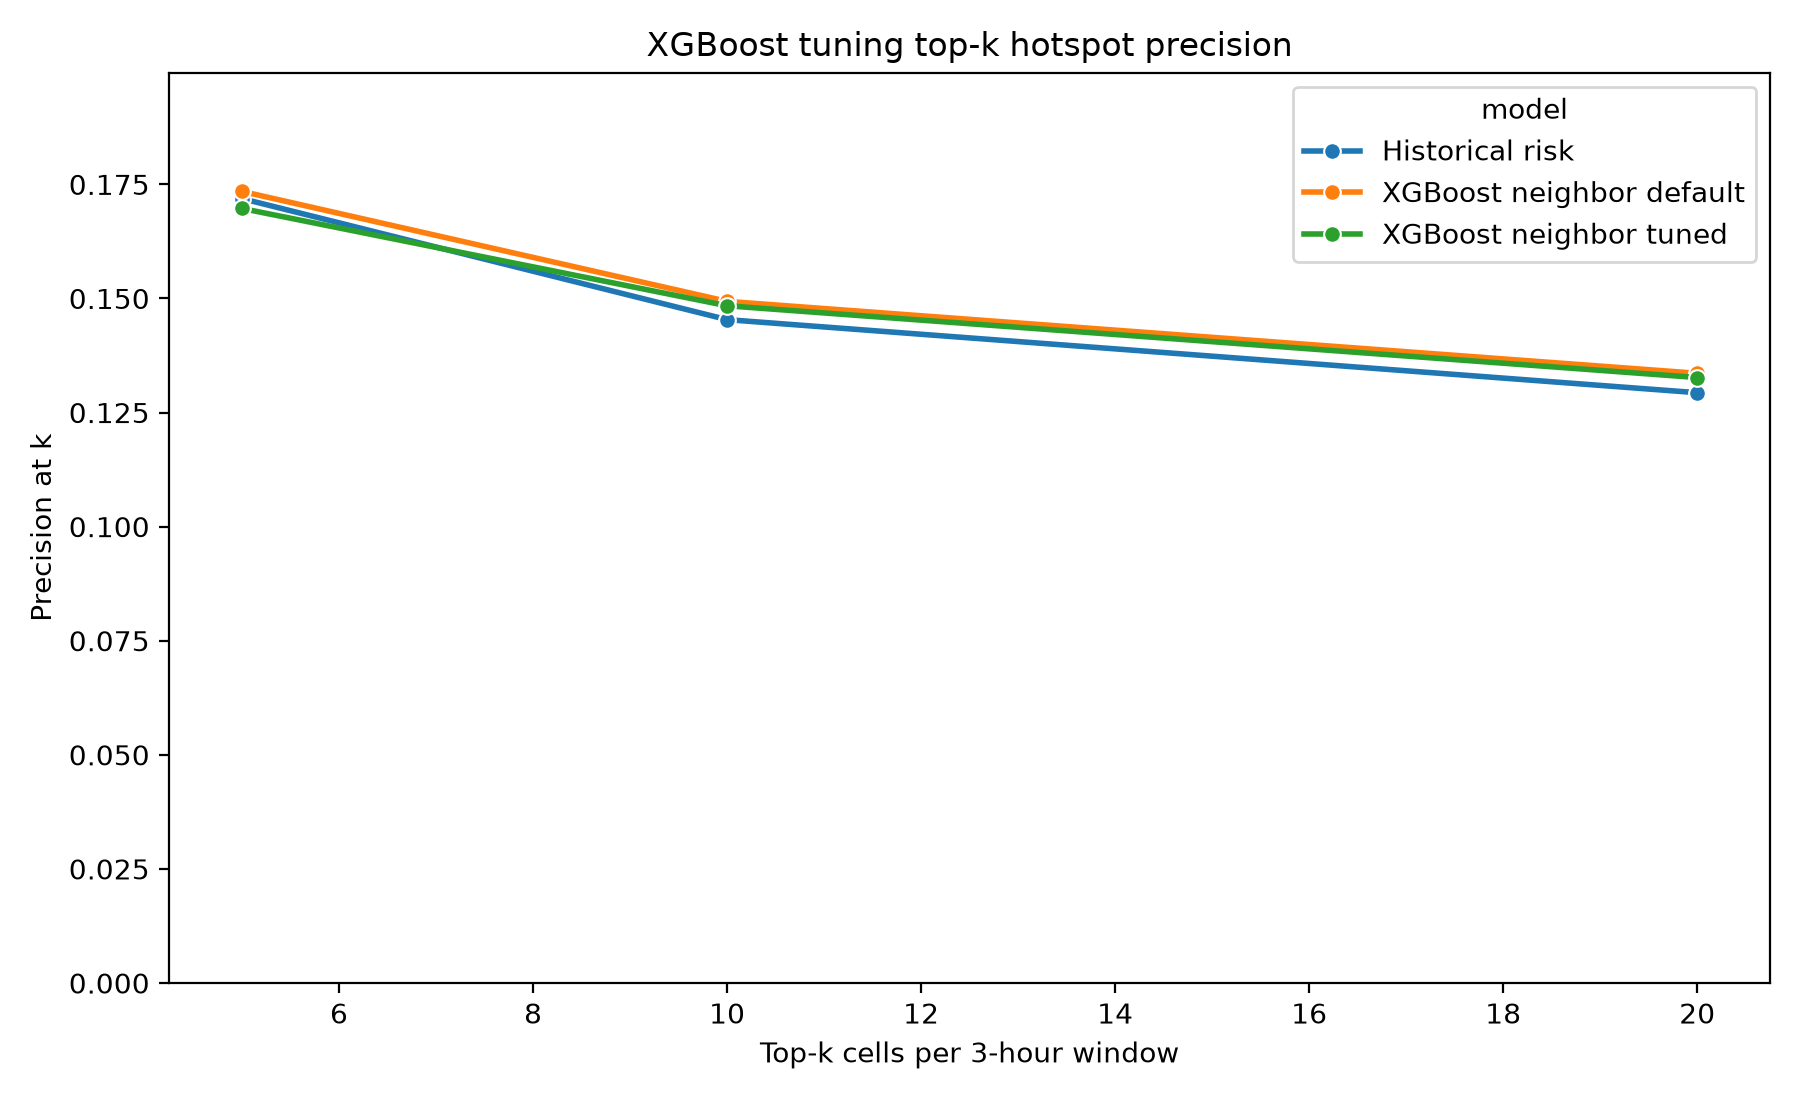
\includegraphics[width=0.88\textwidth]{xgboost_tuning_topk_comparison.png}
\caption{XGBoost tuning top-k comparison}
\label{fig:xgboost_tuning_topk_comparison}
\end{figure}

\FloatBarrier

\section{XGBoost probability calibration experiment}

The default neighbor-feature XGBoost model produces a probability-like score, but the raw score is not automatically a reliable incident probability. This matters for the dashboard because a map should not show an overconfident risk value if the model score is mainly useful for ranking hotspots. A calibration experiment was therefore run after tuning. The classifier, feature set, training sample, H3 resolution, 3-hour window size, and full-grid validation/test population were kept unchanged.

Two post-processing calibration methods were tested. Sigmoid calibration fits a logistic calibration curve to validation-period predictions. Isotonic calibration fits a non-parametric monotonic curve. Both methods were fitted only on validation predictions and labels. The test period was used only for final reporting.

\begin{table}[H]
\centering
\caption{XGBoost probability calibration result}
\label{tab:xgboost_calibration_metrics}
\small
\begin{tabular}{lrrrrr}
\toprule
\textbf{Score} & \textbf{PR-AUC} & \textbf{F1} & \textbf{Brier score} & \textbf{Log loss} & \textbf{ECE} \\
\midrule
Uncalibrated & 0.0992 & 0.1645 & 0.2127 & 0.5953 & 0.3518 \\
Sigmoid calibrated & 0.0992 & 0.1645 & 0.0227 & 0.0983 & 0.0013 \\
Isotonic calibrated & 0.0976 & 0.1645 & 0.0227 & 0.0979 & 0.0013 \\
\bottomrule
\end{tabular}
\end{table}

The uncalibrated score is strongly overconfident as a probability. In the highest score bin, the mean raw predicted score is 0.8404 while the observed incident rate is 0.0990. After sigmoid calibration, the same high-risk bin has a mean predicted risk of 0.0939 and an observed incident rate of 0.0990. This is a much better dashboard risk value.

\begin{table}[H]
\centering
\caption{Top-20 hotspot ranking after calibration}
\label{tab:xgboost_calibration_topk}
\footnotesize
\begin{tabular}{lrrrr}
\toprule
\textbf{Score} & \textbf{Recall@20} & \textbf{Prec.@20} & \textbf{Hit@20} & \textbf{Incident recall@20} \\
\midrule
Uncalibrated & 0.0844 & 0.1336 & 0.9215 & 0.0903 \\
Sigmoid calibrated & 0.0844 & 0.1336 & 0.9215 & 0.0903 \\
Isotonic calibrated & 0.0847 & 0.1340 & 0.9202 & 0.0905 \\
\bottomrule
\end{tabular}
\end{table}

Sigmoid calibration is selected for dashboard probability display. It reduces the Brier score from 0.2127 to 0.0227 and reduces equal-frequency expected calibration error from 0.3518 to 0.0013, while leaving ROC-AUC, PR-AUC, F1-score, and top-k hotspot ranking unchanged. Isotonic calibration gives a slightly lower log loss and maximum calibration error, but it reduces PR-AUC from 0.0992 to 0.0976. Since the dashboard needs stable calibrated risk values without weakening the ranking metric, sigmoid calibration is the better final choice.

The calibration result separates two ideas that are often confused. Ranking quality asks whether high-risk cells are placed above low-risk cells. Probability reliability asks whether the displayed score matches observed incident rates. The uncalibrated XGBoost model is acceptable for ranking but too confident as a probability. Sigmoid calibration fixes this for dashboard display without changing the hotspot ranking.

\begin{figure}[H]
\centering
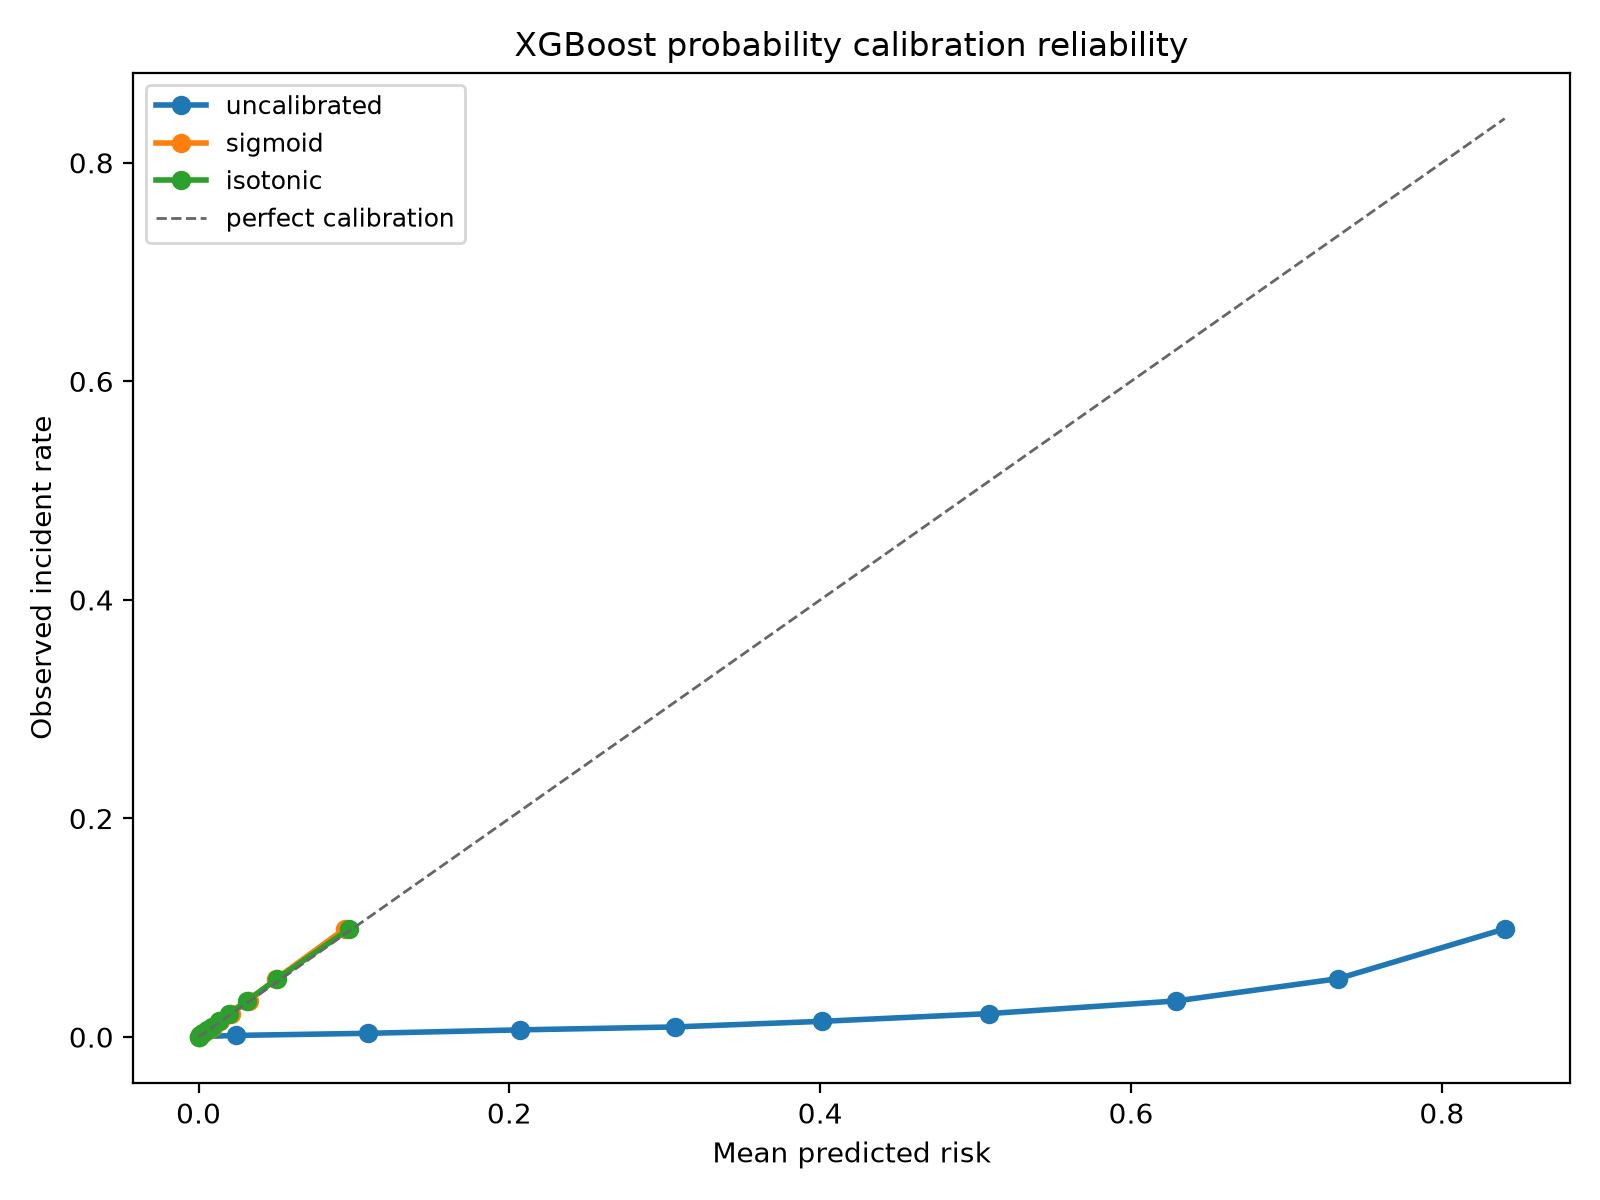
\includegraphics[width=0.82\textwidth]{xgboost_calibration_reliability.png}
\caption{Reliability curve for calibrated XGBoost risk scores}
\label{fig:xgboost_calibration_reliability}
\end{figure}

\begin{figure}[H]
\centering
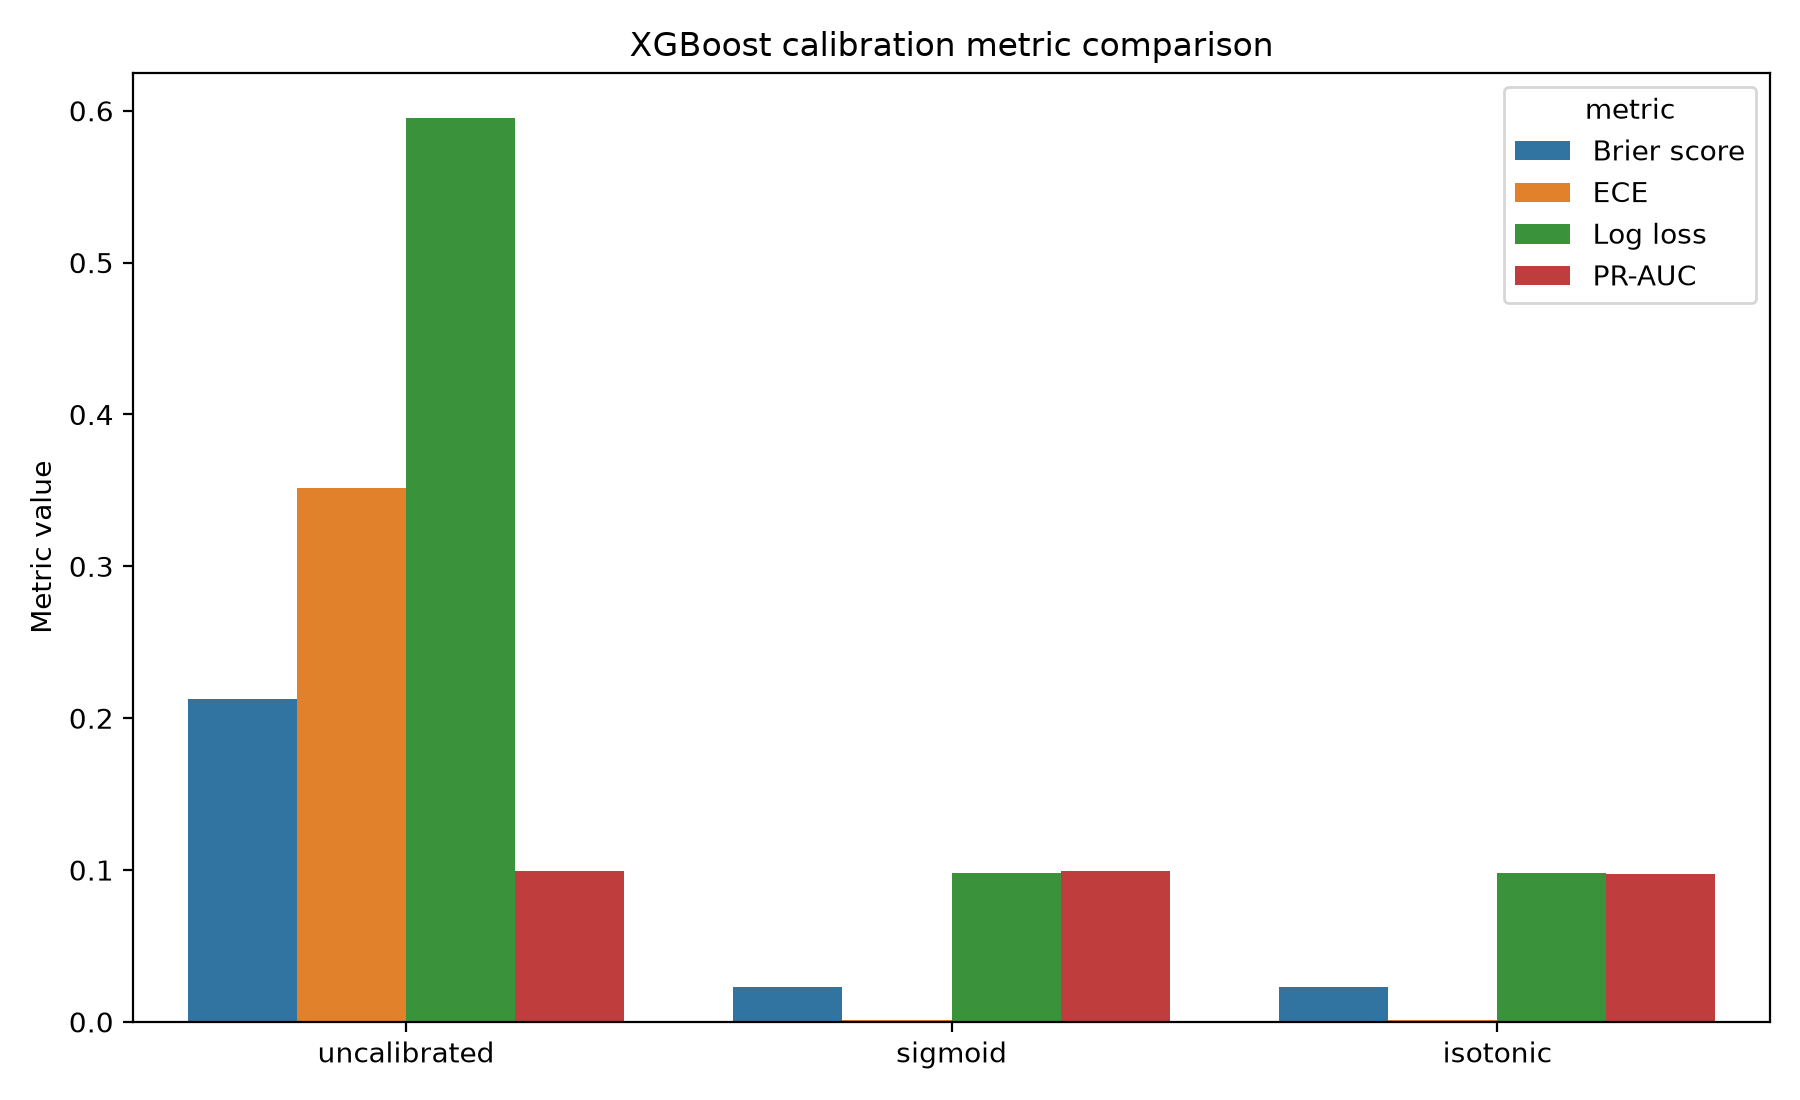
\includegraphics[width=0.82\textwidth]{xgboost_calibration_metric_comparison.png}
\caption{Calibration metric comparison for XGBoost scores}
\label{fig:xgboost_calibration_metric_comparison}
\end{figure}

\begin{figure}[H]
\centering
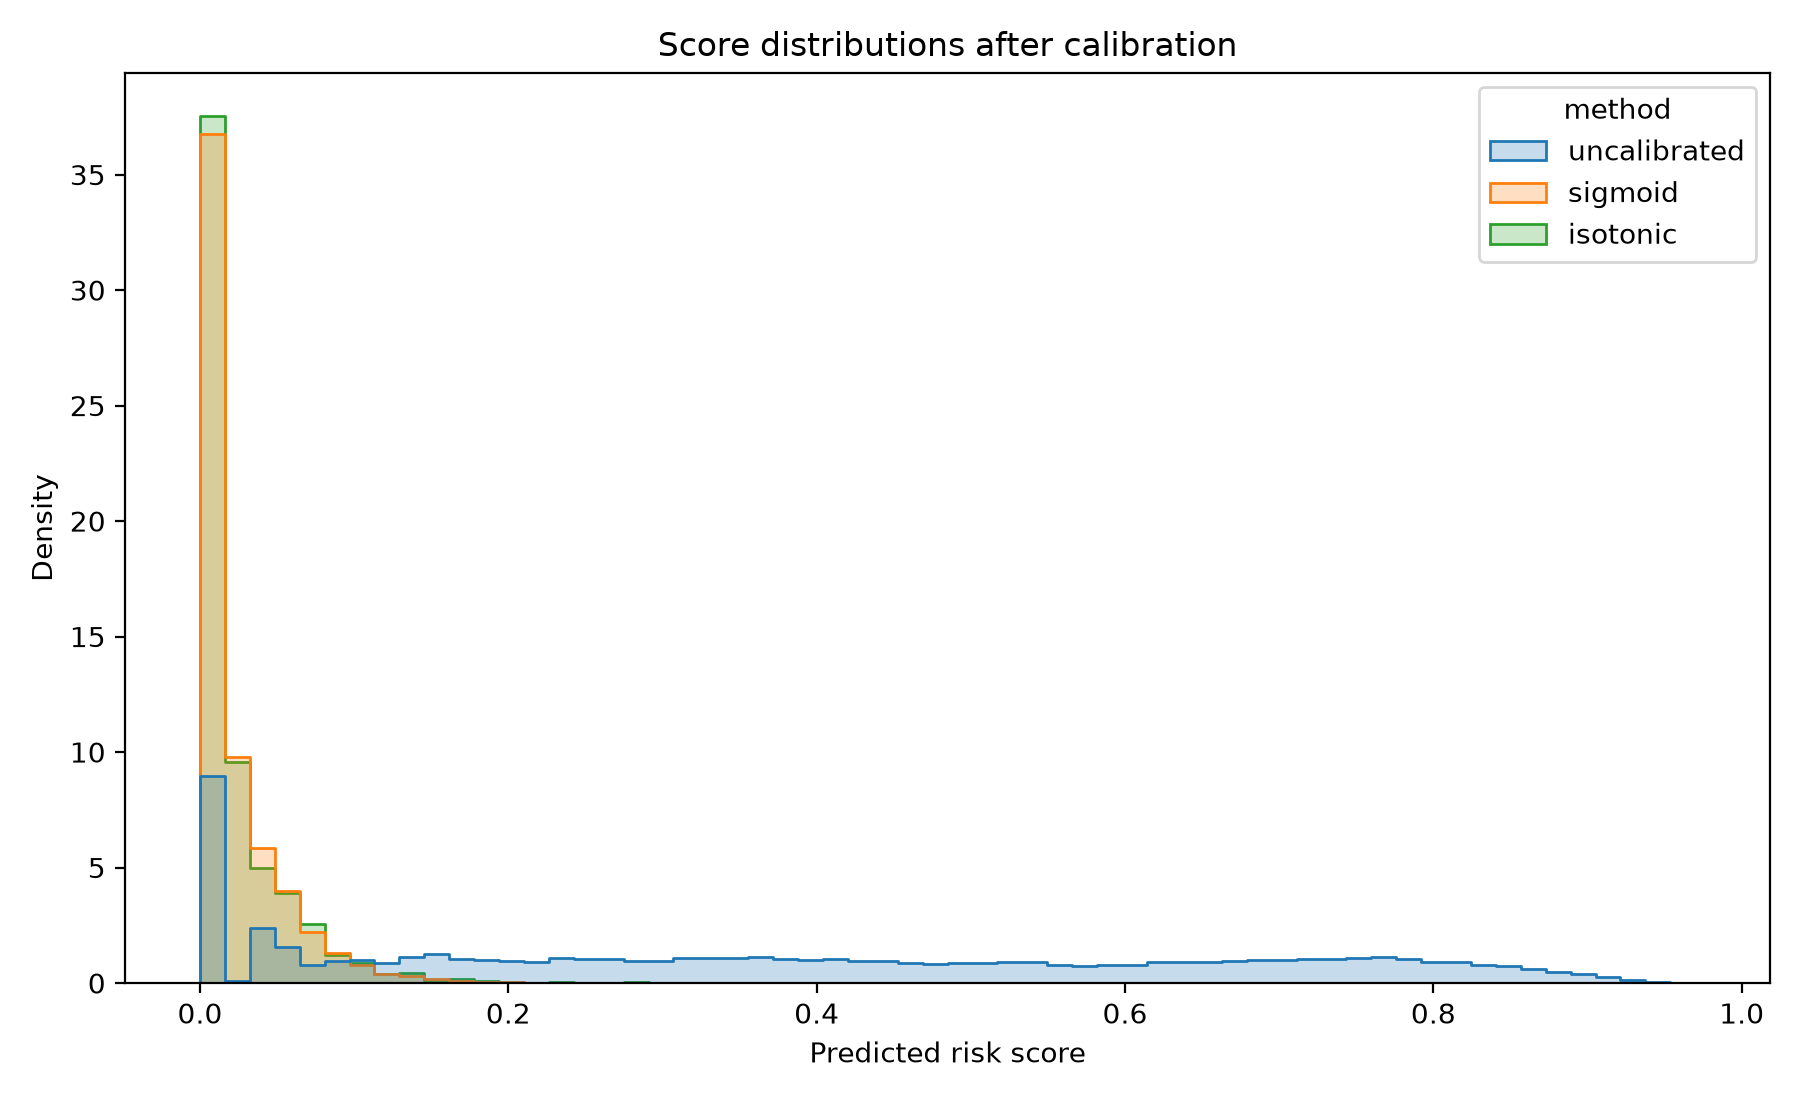
\includegraphics[width=0.82\textwidth]{xgboost_calibration_score_distribution.png}
\caption{Score distribution before and after calibration.}
\label{fig:xgboost_calibration_score_distribution_final}
\end{figure}

\FloatBarrier

\section{Final SHAP and LIME explainability analysis}

After model selection and calibration, SHAP and LIME were rerun for the final selected model: default neighbor-feature XGBoost with H3 resolution 8, 3-hour windows, inside-Dubai cells only, and the existing sampled-negative training table. The rejected hard-negative sample and the tuned XGBoost configuration were not used. SHAP explains the underlying XGBoost raw-margin score. LIME is used as a local model-agnostic comparison. The sigmoid-calibrated probability is reported as the dashboard-facing risk value, not as a separate explanation method.

\begin{table}[H]
\centering
\caption{Top grouped SHAP features for the final XGBoost model}
\label{tab:final_shap_global_features}
\small
\begin{tabular}{lrr}
\toprule
\textbf{Feature group} & \textbf{Mean absolute SHAP} & \textbf{Mean SHAP} \\
\midrule
Historical cell-hour risk & 2.1737 & -1.7115 \\
Year & 0.2534 & 0.2534 \\
Historical cell risk & 0.0988 & -0.0751 \\
Previous 7-day incident count & 0.0937 & -0.0459 \\
Neighbor previous 7-day incident count & 0.0660 & -0.0409 \\
Weekend flag & 0.0494 & 0.0000 \\
Neighbor previous 24-hour incident count & 0.0369 & -0.0121 \\
Day of week & 0.0356 & 0.0003 \\
\bottomrule
\end{tabular}
\end{table}

The SHAP result confirms that the model is driven mainly by historical risk in the same cell and hour block. Recent activity also matters. The final model now uses neighboring-cell features, and those features appear in the global explanation: neighboring 7-day incident count is the fifth strongest grouped feature, and neighboring 24-hour incident count is seventh. This supports the earlier result that nearby recent activity adds a modest but useful spatial signal.

The sign of SHAP values depends on the specific feature value and model context, so the global table is interpreted mainly by mean absolute SHAP. The strongest feature group, historical cell-hour risk, has the largest average contribution magnitude. The model also uses recent same-cell and neighboring-cell incident counts. This matches the intended design: long-term risk gives the baseline, and recent activity adjusts the score around that baseline.

\begin{figure}[H]
\centering
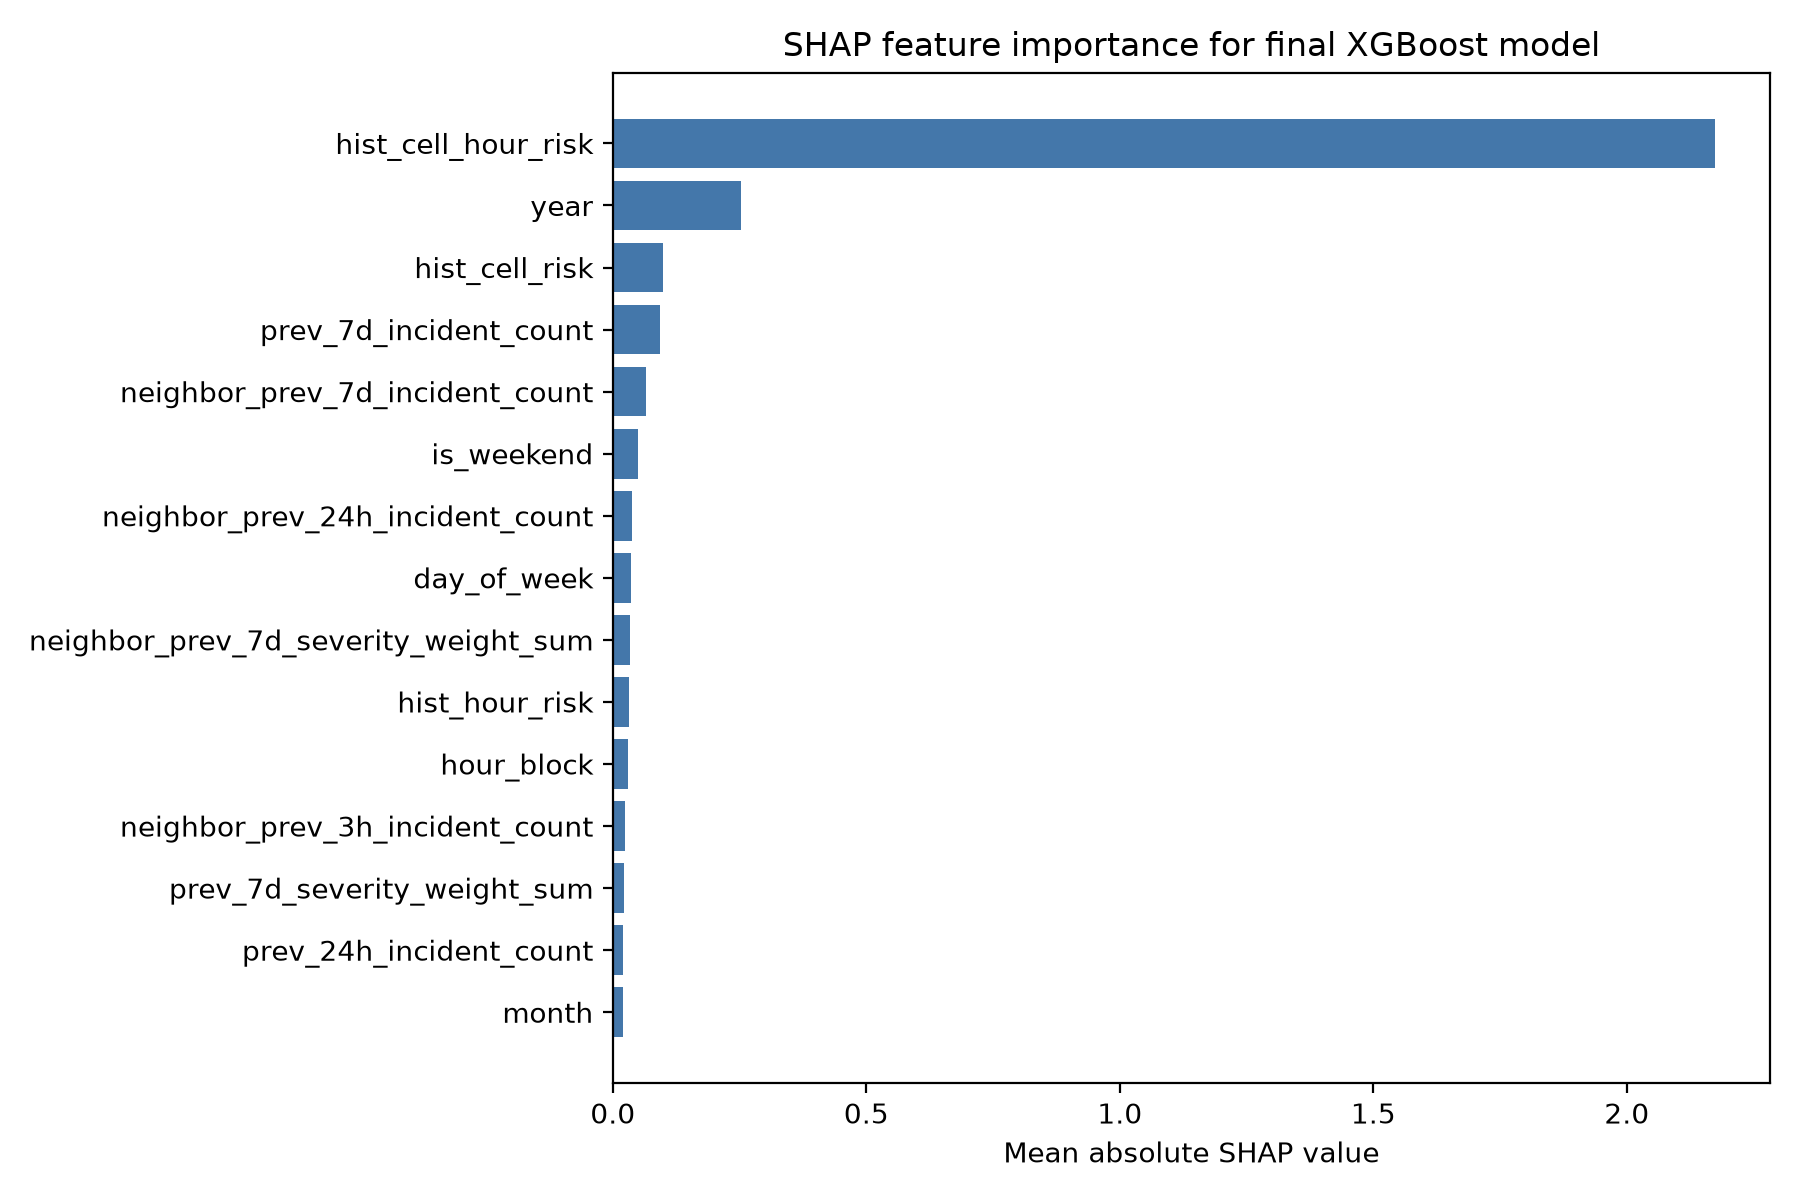
\includegraphics[width=0.88\textwidth]{shap_feature_importance_bar.png}
\caption{SHAP feature importance for the final neighbor-feature XGBoost model}
\label{fig:final_shap_feature_importance}
\end{figure}

\begin{figure}[H]
\centering
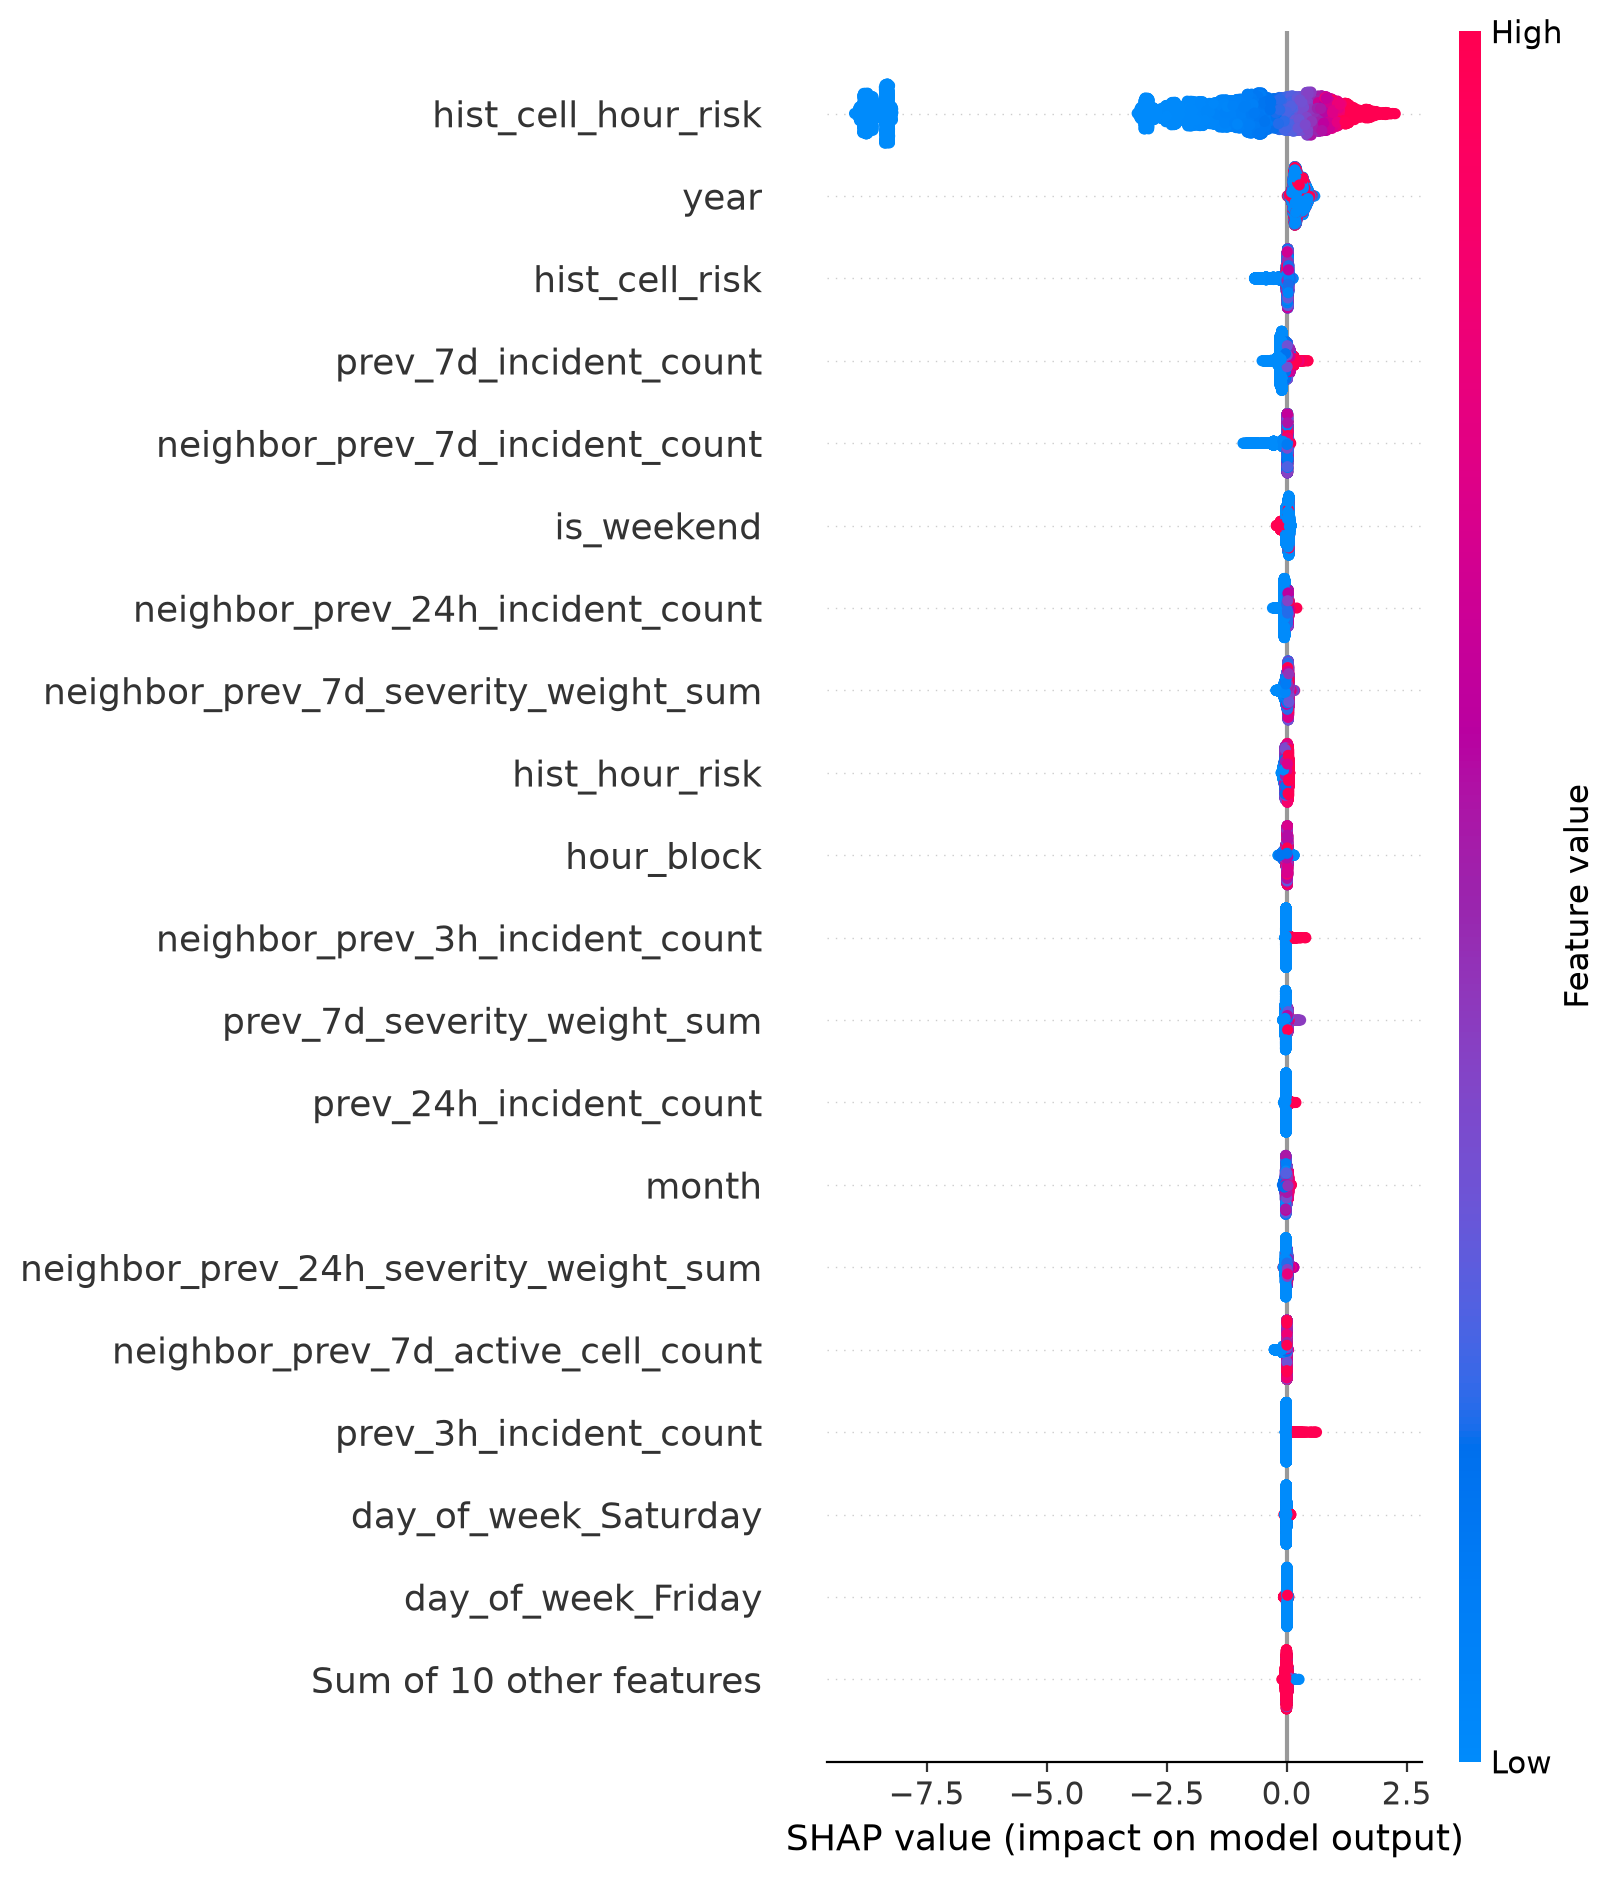
\includegraphics[width=0.88\textwidth]{shap_beeswarm.png}
\caption{SHAP beeswarm plot for final-model test candidates}
\label{fig:final_shap_beeswarm}
\end{figure}

\begin{table}[H]
\centering
\caption{Final local explanation cases}
\label{tab:final_local_explanation_cases}
\small
\begin{tabular}{lrrrr}
\toprule
\textbf{Case} & \textbf{Actual} & \textbf{Raw score} & \textbf{Calibrated risk} & \textbf{Predicted} \\
\midrule
High-risk true positive & 1 & 0.9714 & 0.3505 & 1 \\
High-risk false positive & 0 & 0.9739 & 0.3707 & 1 \\
Low-score false negative & 1 & 0.0001 & 0.0000 & 0 \\
Low-risk true negative & 0 & 0.0001 & 0.0000 & 0 \\
\bottomrule
\end{tabular}
\end{table}

The two high-risk examples are driven by high historical cell-hour risk, high previous 7-day incident counts, and recent neighboring-cell activity. The false positive has the same pattern as the true positive, which is useful diagnostically: the model identifies a historically risky local context, but no incident occurs in that particular cell/window. The false negative and true negative both have zero historical cell-hour risk and little recent local or neighboring activity, so the model assigns very low risk.

\begin{table}[H]
\centering
\caption{SHAP and LIME agreement on selected local cases}
\label{tab:final_lime_shap_comparison}
\footnotesize
\begin{tabularx}{\textwidth}{L{0.25\textwidth}rY}
\toprule
\textbf{Case} & \textbf{Top-5 overlap} & \textbf{Shared explanation pattern} \\
\midrule
High-risk true positive & 5 & Historical cell-hour risk and recent incident history raise risk. \\
High-risk false positive & 4 & Historical cell-hour risk, recent incidents, and neighbor activity raise risk. \\
Low-score false negative & 4 & Zero historical risk and low recent activity reduce risk. \\
Low-risk true negative & 4 & Zero historical risk and low recent activity reduce risk. \\
\bottomrule
\end{tabularx}
\end{table}

SHAP and LIME broadly agree on the main local drivers. SHAP is retained as the main explanation method because it gives a consistent global ranking and local attributions for the tree model. LIME is kept as supporting evidence because it gives a model-agnostic local check requested during supervisor feedback. Neither method should be interpreted causally; both describe how the trained model uses the available features.

The local examples make the model's behavior more concrete. The high-risk true positive and high-risk false positive both have high historical cell-hour risk and recent incident activity. The model therefore raises the risk score in both cases. The difference is that one window contains an actual incident and the other does not. This is expected in a probabilistic risk task. The low-score false negative shows the opposite failure mode: an incident occurs in a cell/window where the model sees little historical or recent warning.

\begin{figure}[H]
\centering
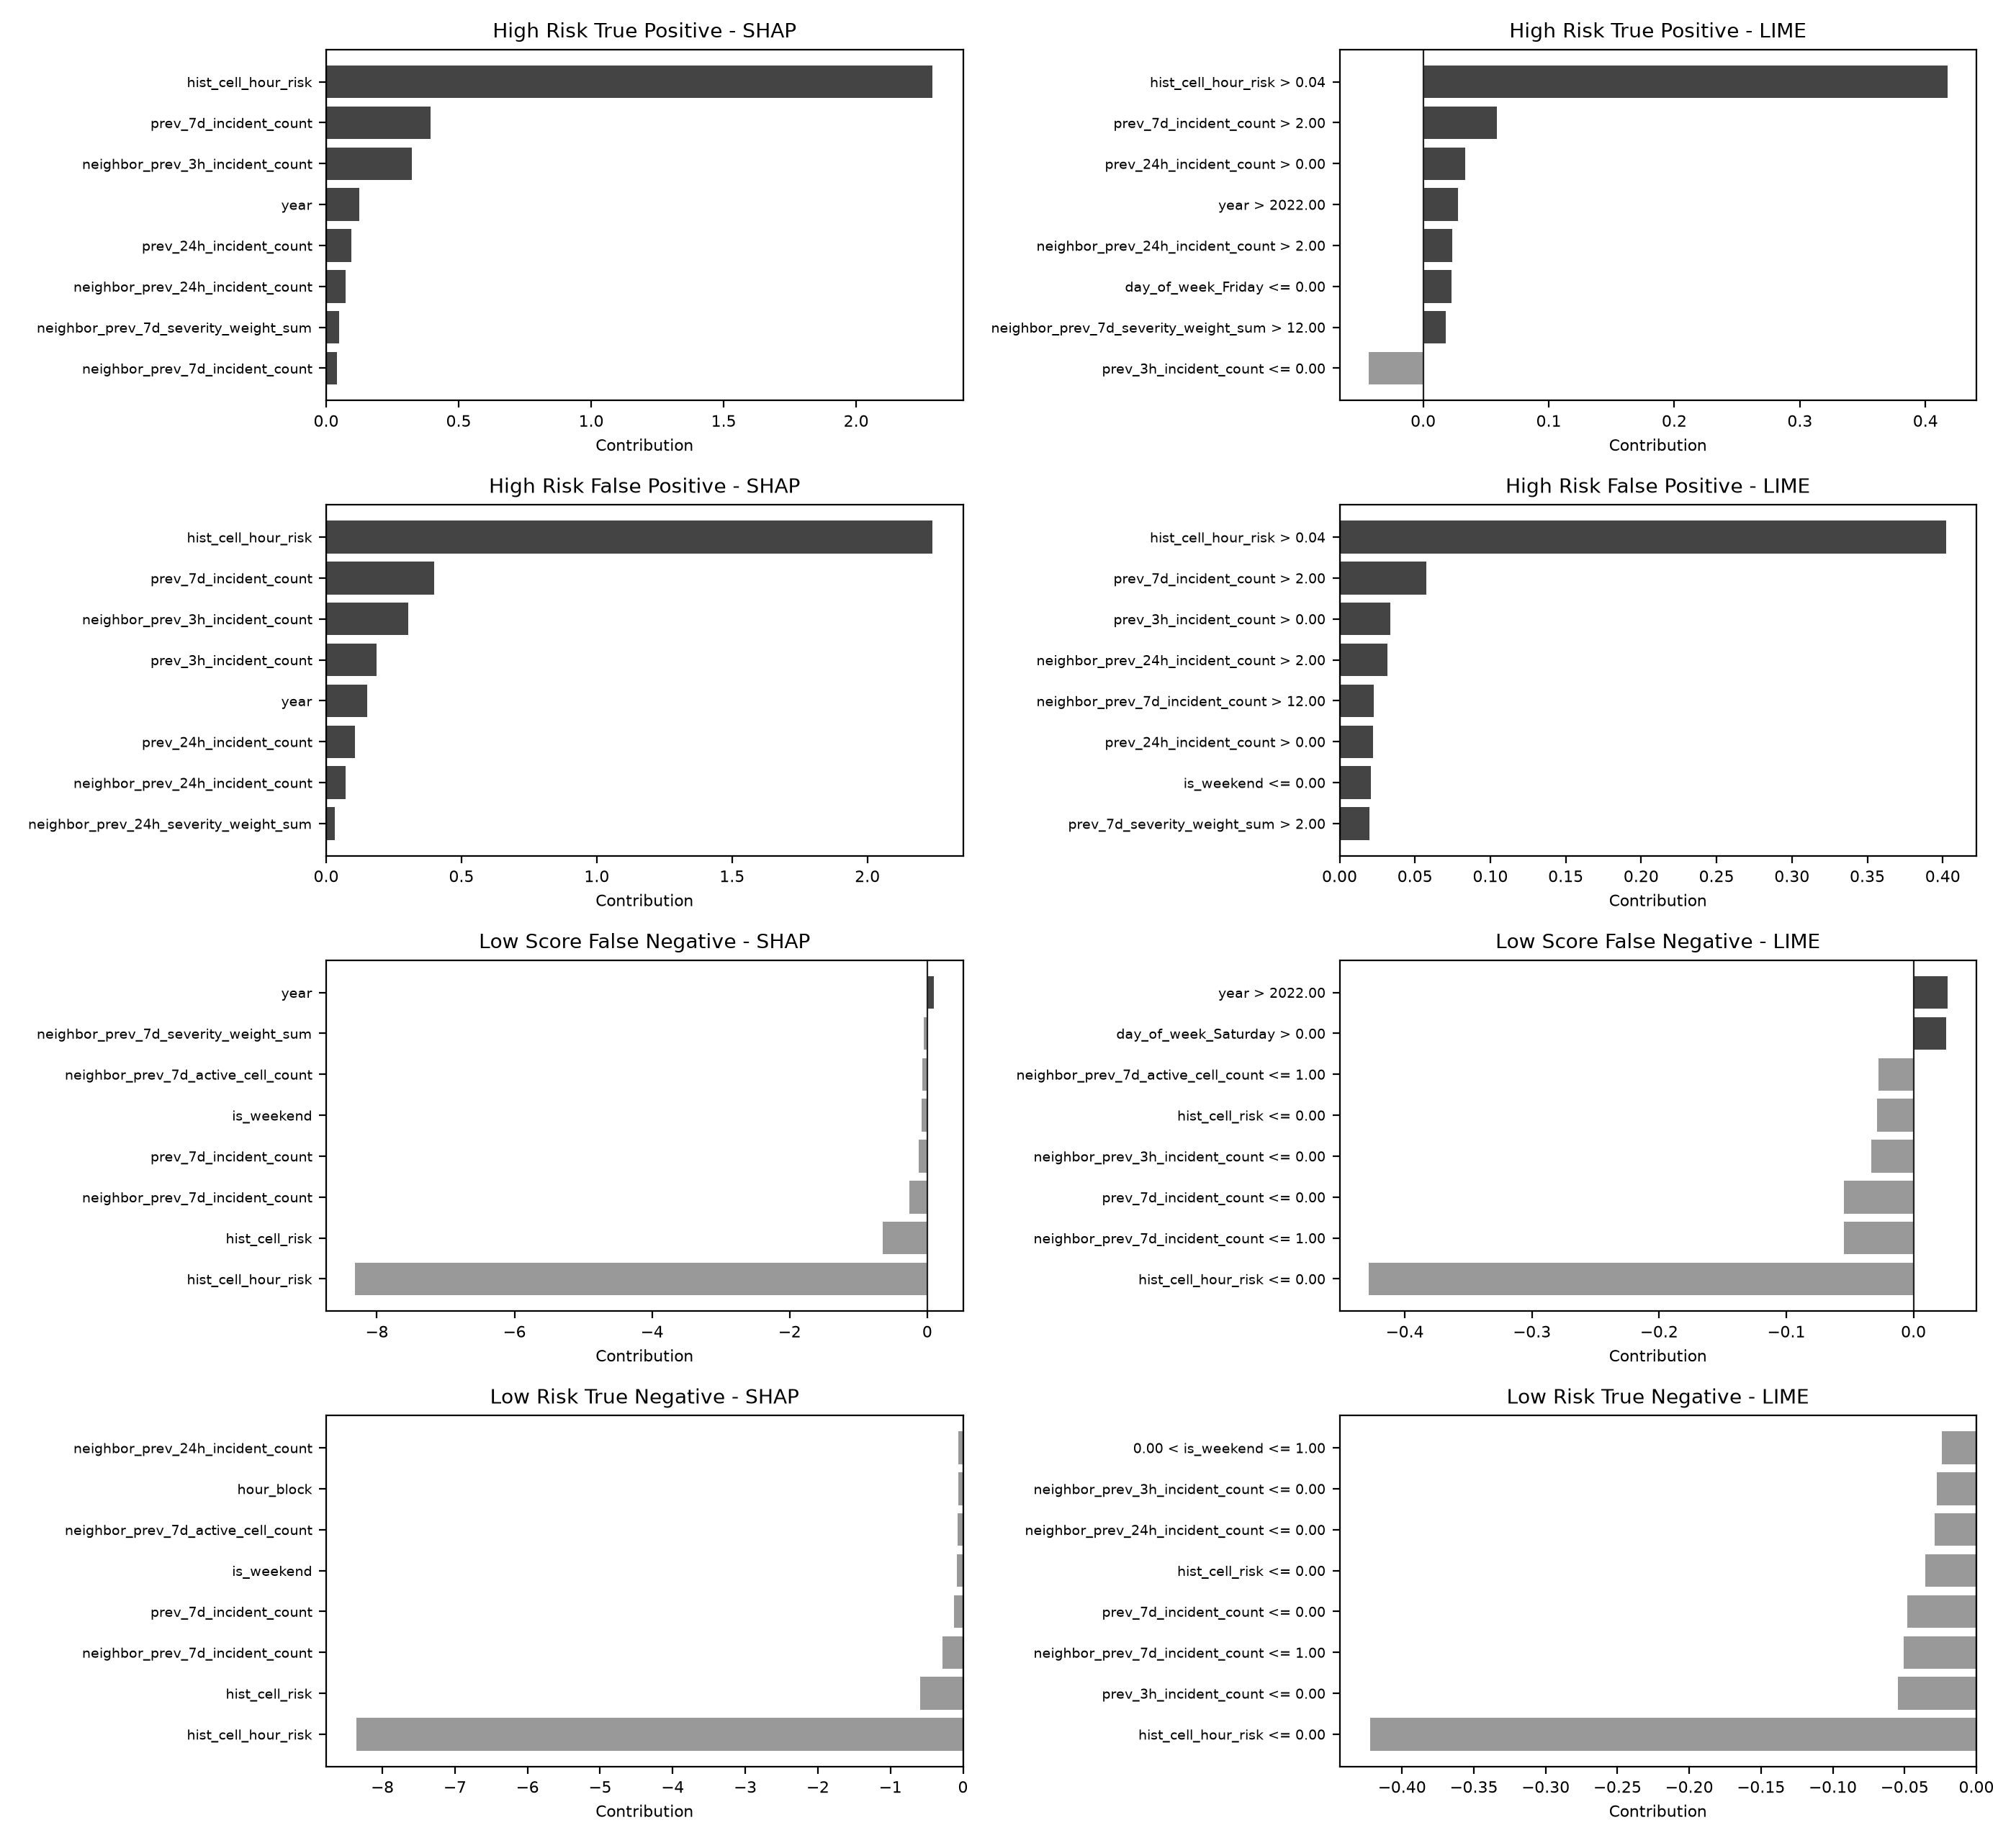
\includegraphics[width=0.9\textwidth]{lime_shap_local_comparison.png}
\caption{Final LIME and SHAP local explanation comparison}
\label{fig:final_lime_shap_comparison}
\end{figure}

\begin{figure}[H]
\centering
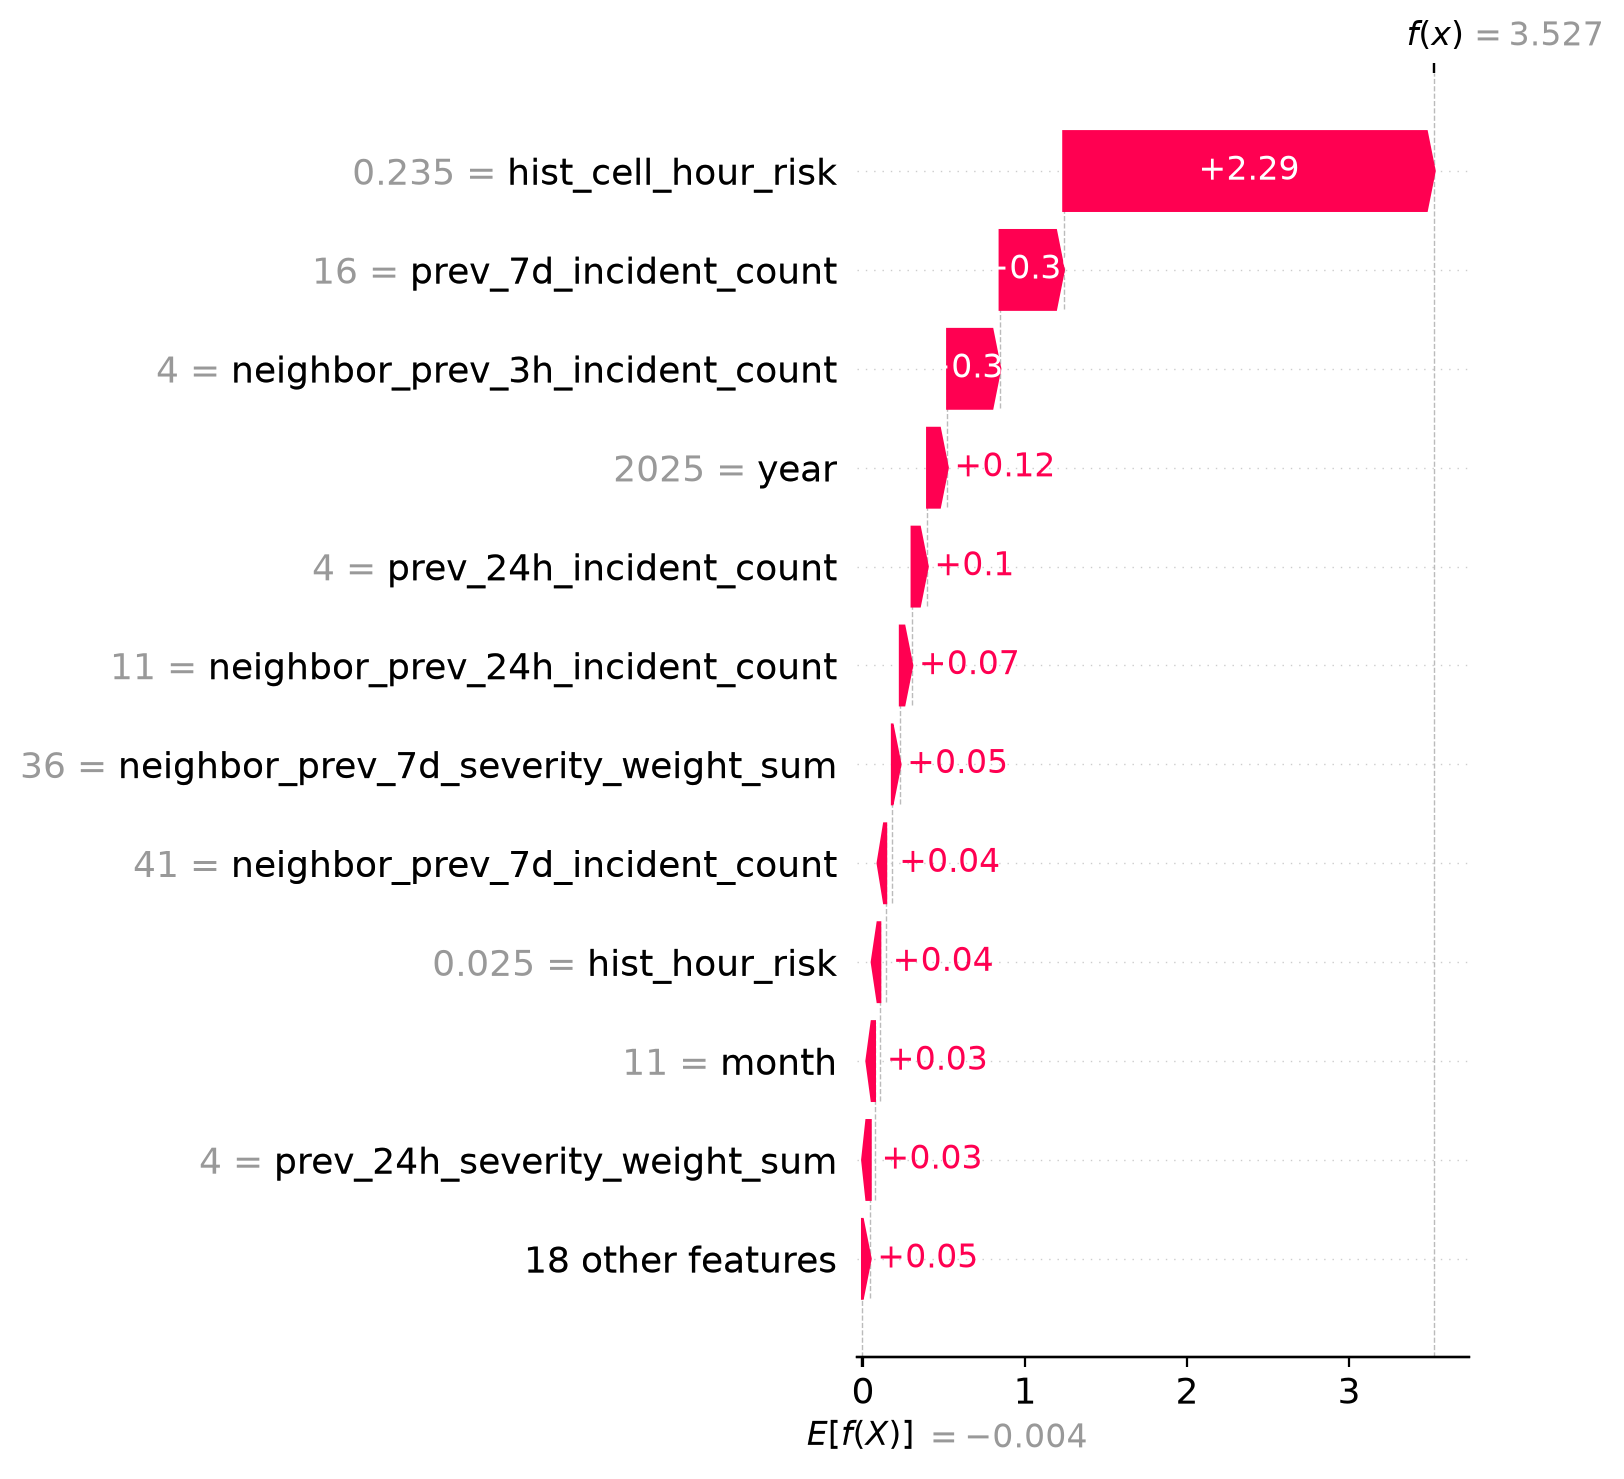
\includegraphics[width=0.82\textwidth]{shap_local_high_risk_tp.png}
\caption{Local SHAP explanation for the high-risk true-positive case.}
\label{fig:shap_local_high_risk_tp_final}
\end{figure}

\begin{figure}[H]
\centering
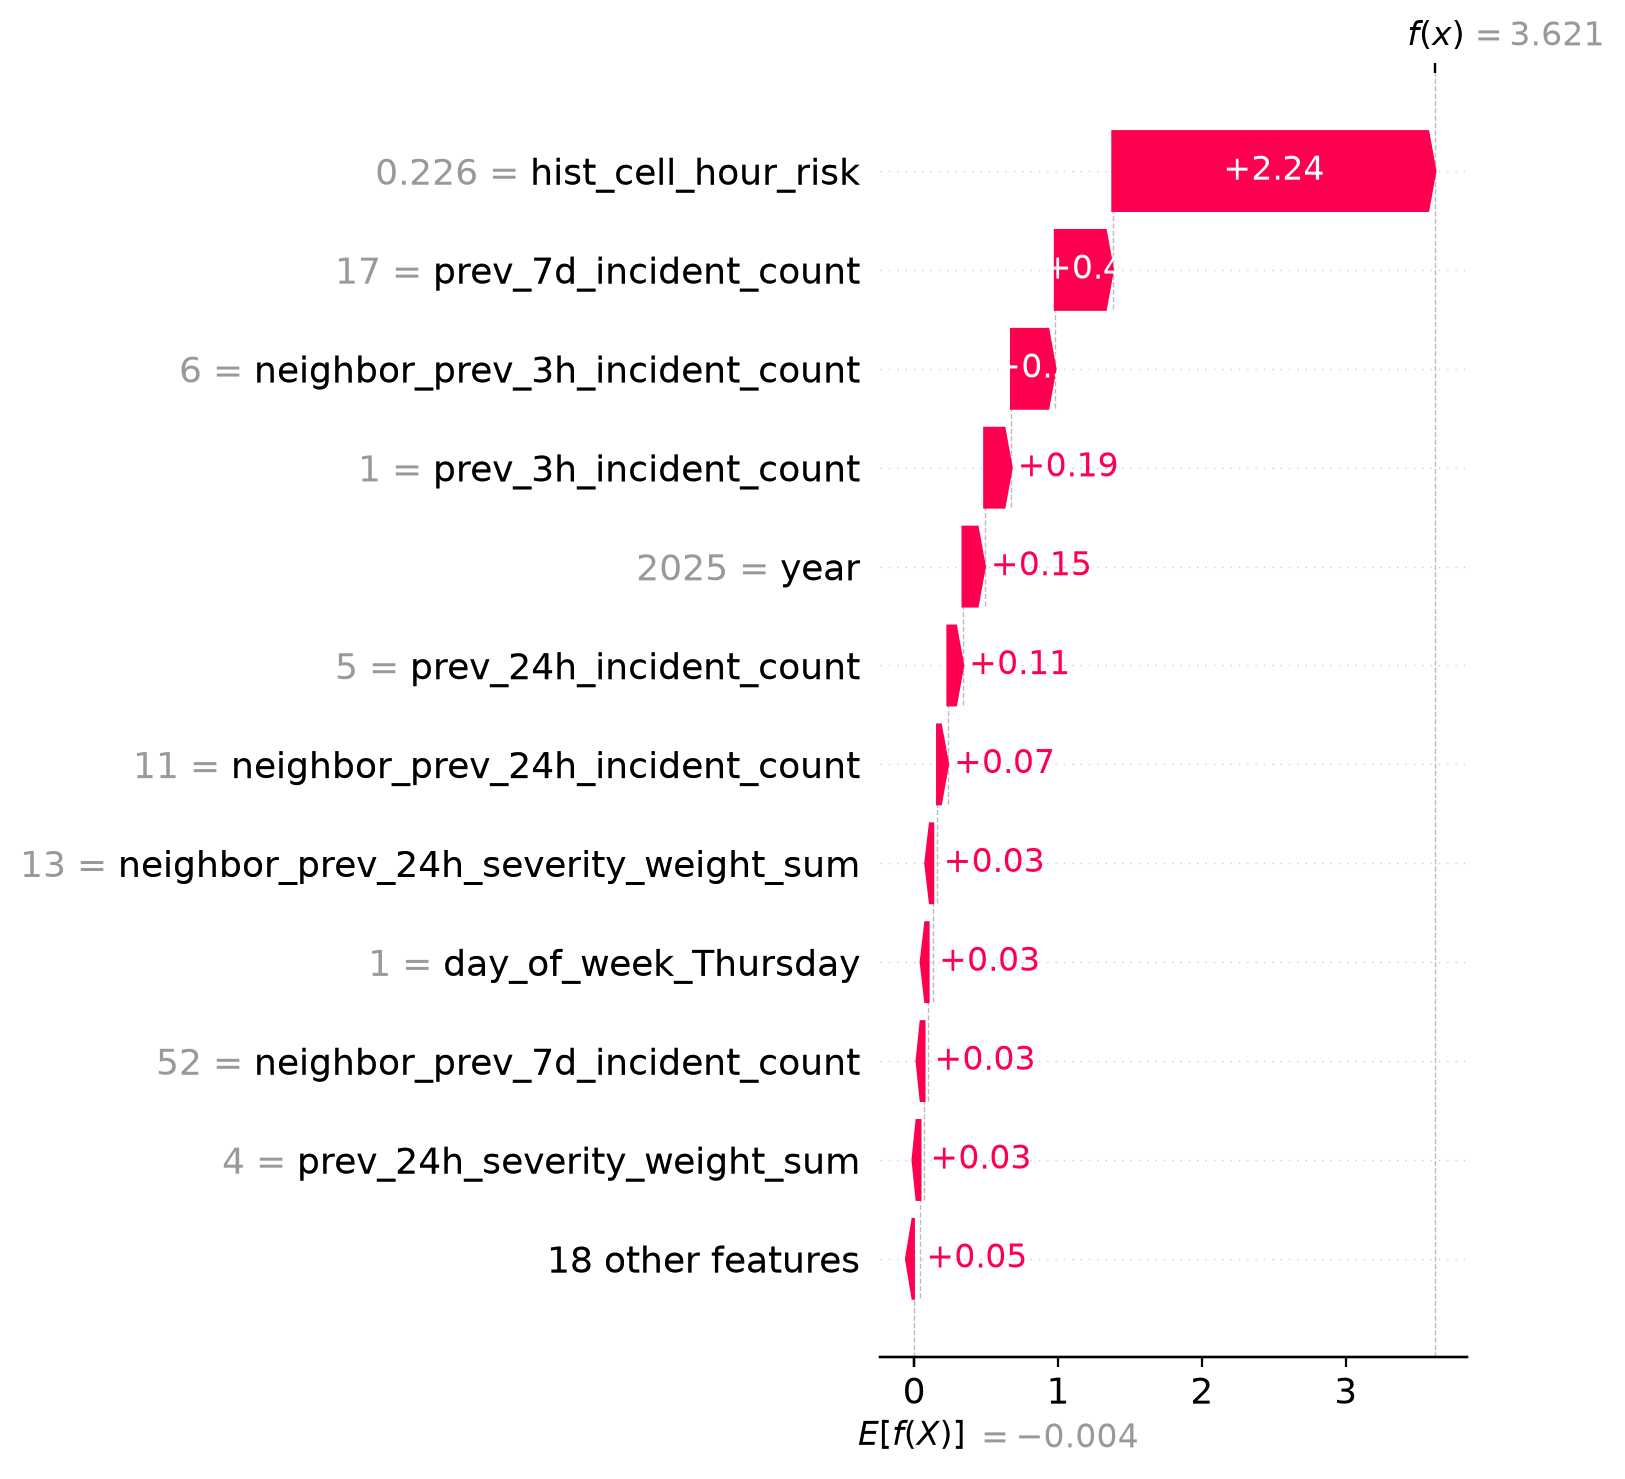
\includegraphics[width=0.82\textwidth]{shap_local_false_positive.png}
\caption{Local SHAP explanation for the high-risk false-positive case.}
\label{fig:shap_local_false_positive_final}
\end{figure}

\begin{figure}[H]
\centering
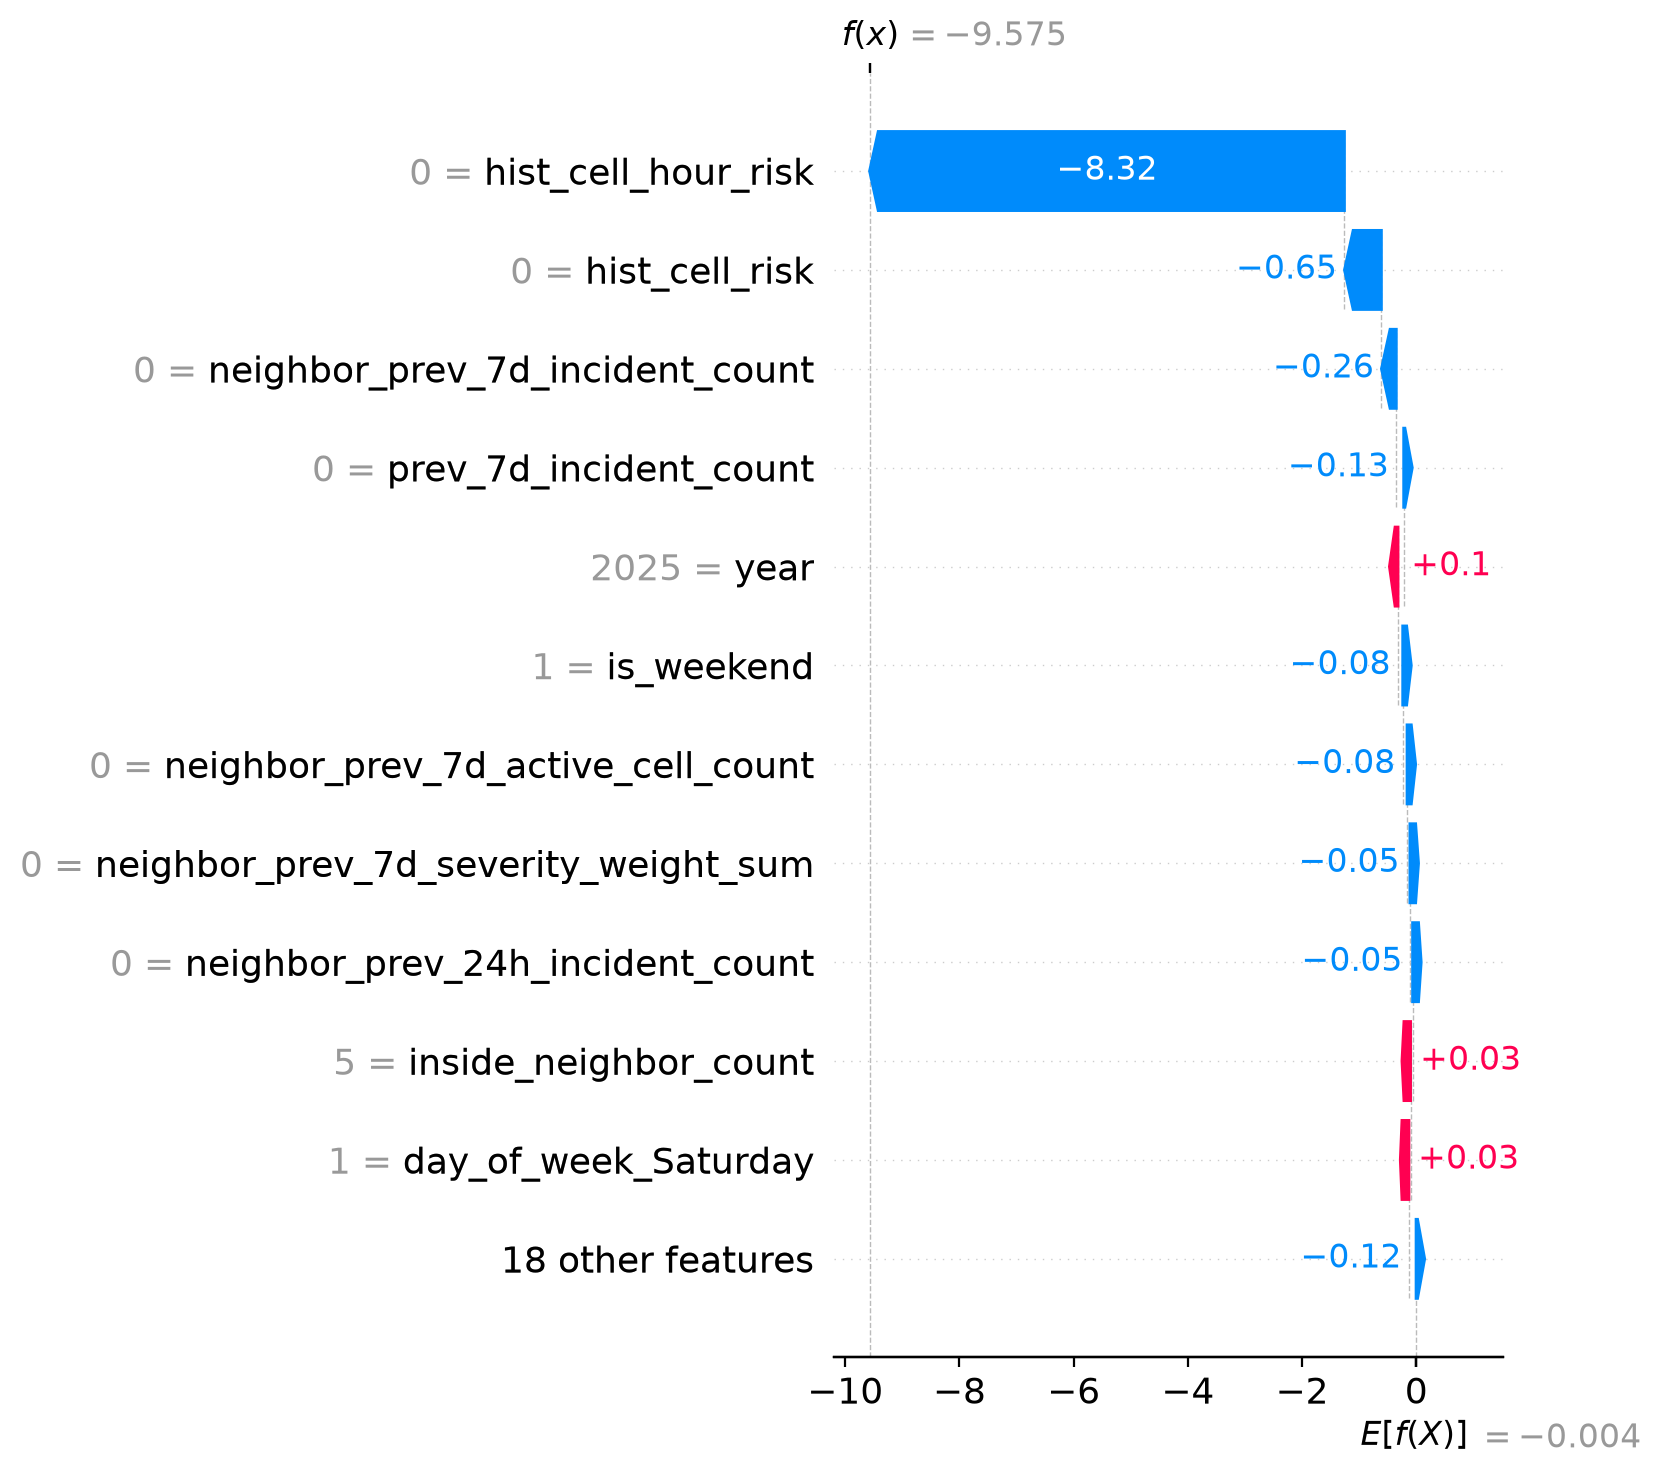
\includegraphics[width=0.82\textwidth]{shap_local_false_negative.png}
\caption{Local SHAP explanation for the low-score false-negative case.}
\label{fig:shap_local_false_negative_final}
\end{figure}

\begin{figure}[H]
\centering
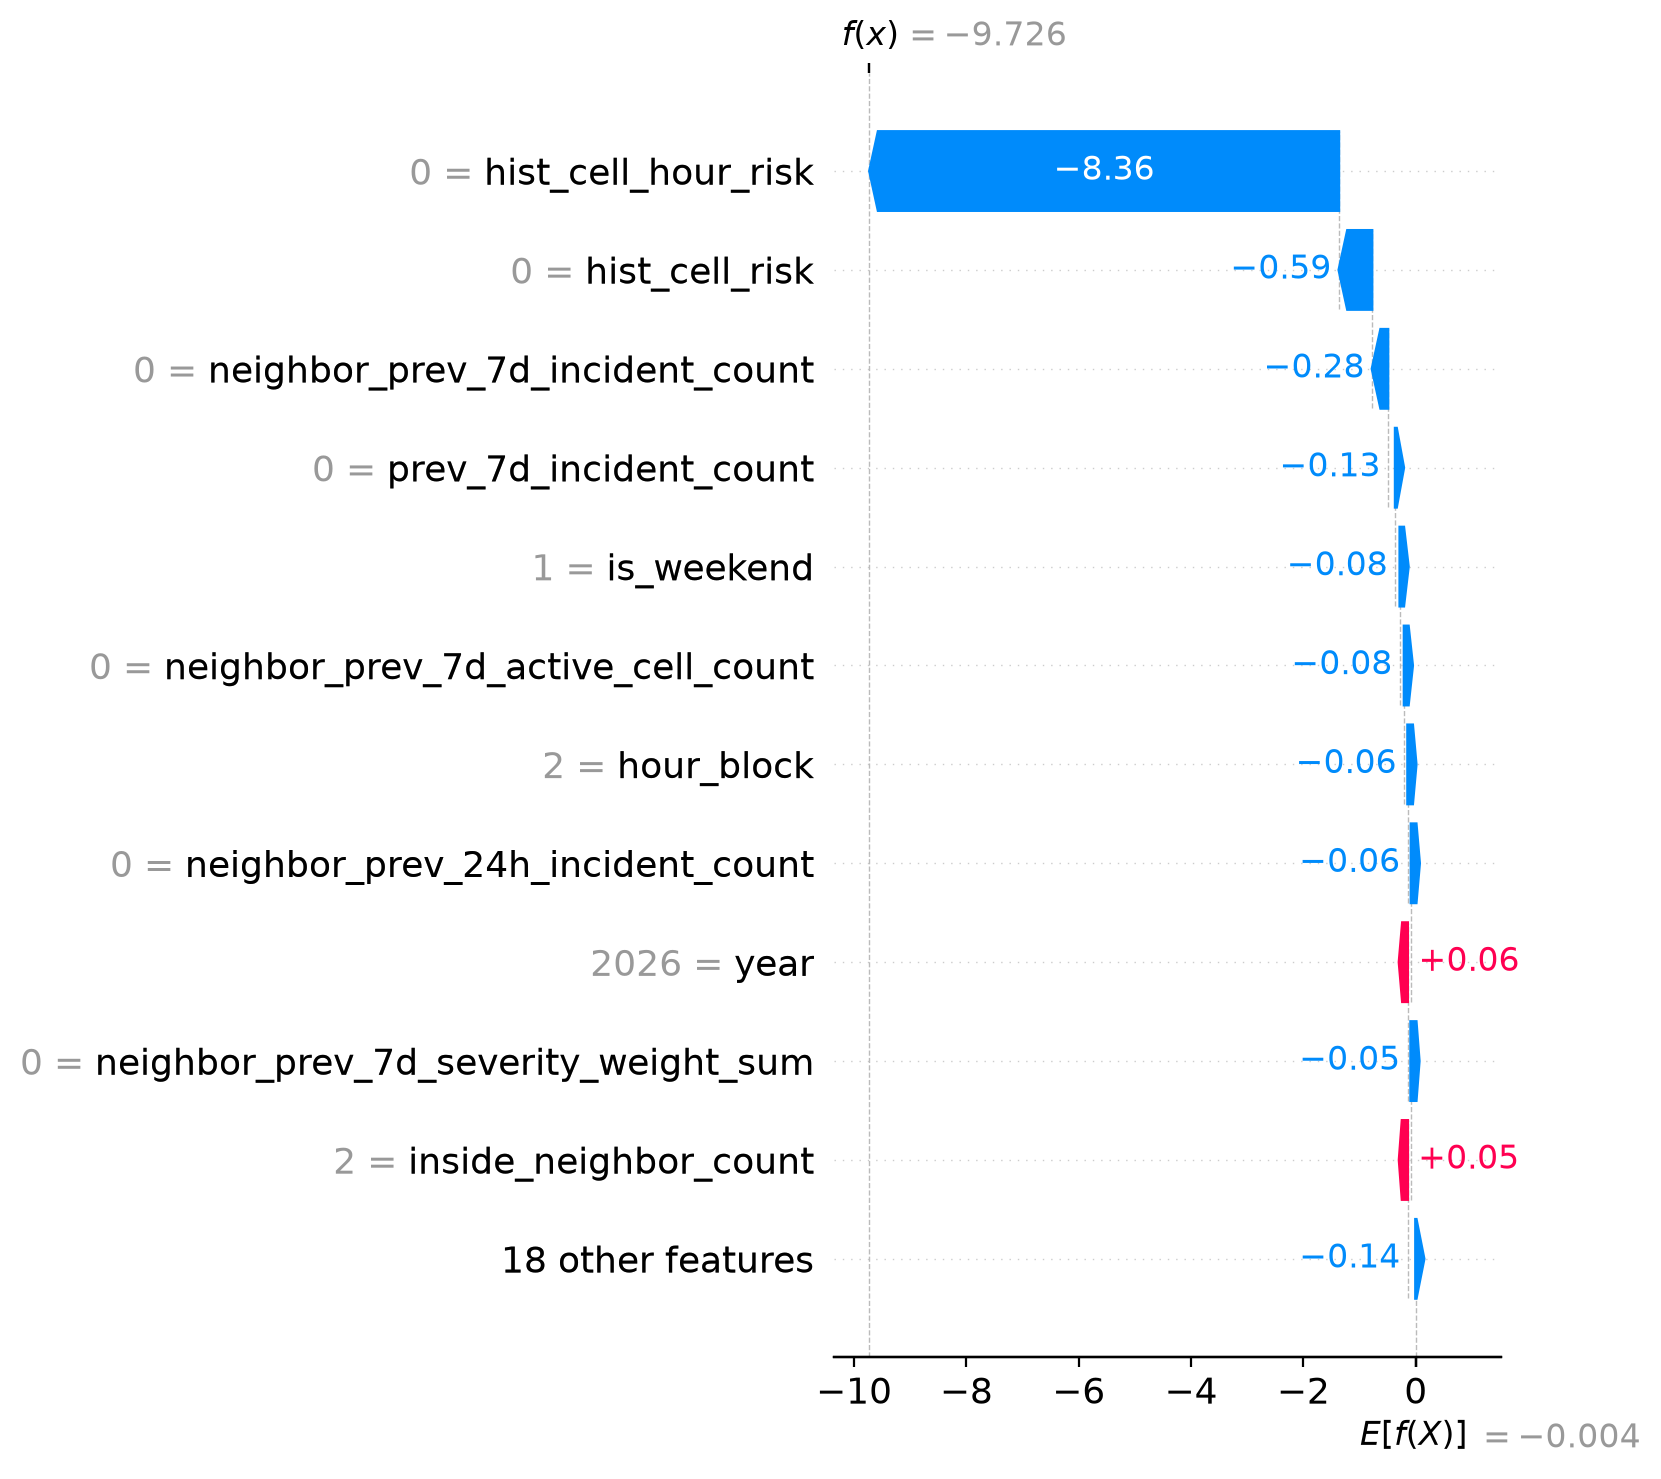
\includegraphics[width=0.82\textwidth]{shap_local_true_negative.png}
\caption{Local SHAP explanation for the low-risk true-negative case.}
\label{fig:shap_local_true_negative_final}
\end{figure}

\FloatBarrier

\section{Implication for final model selection}

The neighbor-feature experiment supports the use of short-range spatial history in the final modeling path. The hard-negative experiment does not support changing the training sample in its current 70/30 form, and the tested hyperparameter tuning run does not improve the untouched test result. The final model selection therefore keeps the default neighbor-feature XGBoost trained on the existing sampled-negative table as the current strongest experiment. For dashboard display, the model's raw score should be passed through sigmoid calibration before being shown as a probability-like risk value. SHAP is the main explanation method for the selected model, with LIME used as a supporting local comparison.

\chapter{Dashboard demonstration}

The dashboard is the practical demonstration layer for the thesis. It lets a supervisor, examiner, or technical reviewer inspect the model output without reading the modeling code. The dashboard does not claim live traffic monitoring or operational deployment. It uses the frozen historical incident snapshot, the selected inside-Dubai H3 resolution-8 grid, 3-hour windows, sigmoid-calibrated XGBoost risk values, and SHAP explanations.

\section{Dashboard purpose}

The purpose of the dashboard is to translate the modeling result into three simple questions:

\begin{enumerate}
    \item Where does the model rank incident risk highest?
    \item When does the selected risk window occur?
    \item Why does the model rank a selected zone and time as risky?
\end{enumerate}

These questions are easier to defend than a generic model-results page. The dashboard is not meant to show every row of the full test matrix. It focuses on ranked zones, map inspection, and explanation. The scientific evidence remains available in separate views, but the first interaction is centered on the prediction output.

\section{Rolling replay concept}

The main dashboard view is a rolling replay. It uses the final selected model, the default neighbor-feature XGBoost classifier, on complete observed days near the end of the available data. The replay is not a long-range forecast after the source-data cutoff. It is a historical demonstration of how the selected model behaves when the required recent lag features are available.

This design choice is important. The final model uses previous 3-hour, 24-hour, and 7-day incident counts for the same H3 cell and for neighboring H3 cells. These features can be computed for historical replay windows because the previous windows are known. They cannot be computed for dates after 1 June 2026 unless updated incident records are supplied. Showing a post-cutoff date without those updated records would either require a simplified model or missing lag features. The dashboard avoids that confusion and states the data-update requirement directly.

\section{Implementation structure}

The dashboard is implemented with Streamlit, PyDeck, and Plotly. It uses compact precomputed data instead of loading the raw incident file or the full 4.46 million-row historical test matrix during interaction. This keeps the application responsive while preserving the same grid and time-window formulation used in the modeling chapters.

The dashboard has five views:

\begin{enumerate}
    \item \textbf{Rolling replay}: date selector, 3-hour time-window selector, English dashboard map, top-ranked H3 zones, calibrated risk values, known replay outcomes, and a warning about post-cutoff forecasting.
    \item \textbf{Zone explanation}: the same replay controls, top SHAP reasons, feature values, and a local SHAP contribution chart for the selected zone.
    \item \textbf{Historical check}: comparison between ranked H3-cell predictions and known test-period outcomes.
    \item \textbf{Model evidence}: dataset summaries, EDA charts, full-grid evaluation metrics, hotspot ranking, and calibration reliability.
    \item \textbf{Scope notes}: limitations and deployment boundaries.
\end{enumerate}

The map uses a MapTiler vector style rendered through PyDeck. This was chosen because generic free raster basemaps can show local-language street labels in Dubai. H3 polygons are drawn over the MapTiler map, and the user can zoom, pan, inspect ranked zones, and select a zone for explanation. The displayed risk value is the sigmoid-calibrated XGBoost probability. SHAP is used for dashboard explanations because it is stable for the selected tree-based model and can explain the same model used for ranking. LIME remains a report-level comparison on selected local cases.

\section{Dashboard data flow}

The dashboard data is prepared offline. The preparation step retrains and scores the final default neighbor-feature XGBoost model, applies sigmoid calibration for displayed risk values, keeps compact top-risk records for replay windows, stores H3 polygons, and stores SHAP contributor rows for the displayed zones. The dashboard then reads these compact files at runtime.

This design avoids two problems. First, the dashboard does not need to retrain the model when opened. Second, it does not need to load the full raw incident file or the full-grid test matrix. The model evidence shown in the dashboard still matches the thesis results because the compact files are generated from the same final model path.

\section{Dashboard screenshots}

Figure~\ref{fig:dashboard-rolling-replay} shows the default replay page. The default replay date is selected automatically as the latest complete observed day before the data cutoff. The map uses MapTiler English labels and displays the highest-ranked H3 zones for the selected replay date. The visible message tells the reader that later forecasts require updated incident data.

\begin{figure}[H]
    \centering
    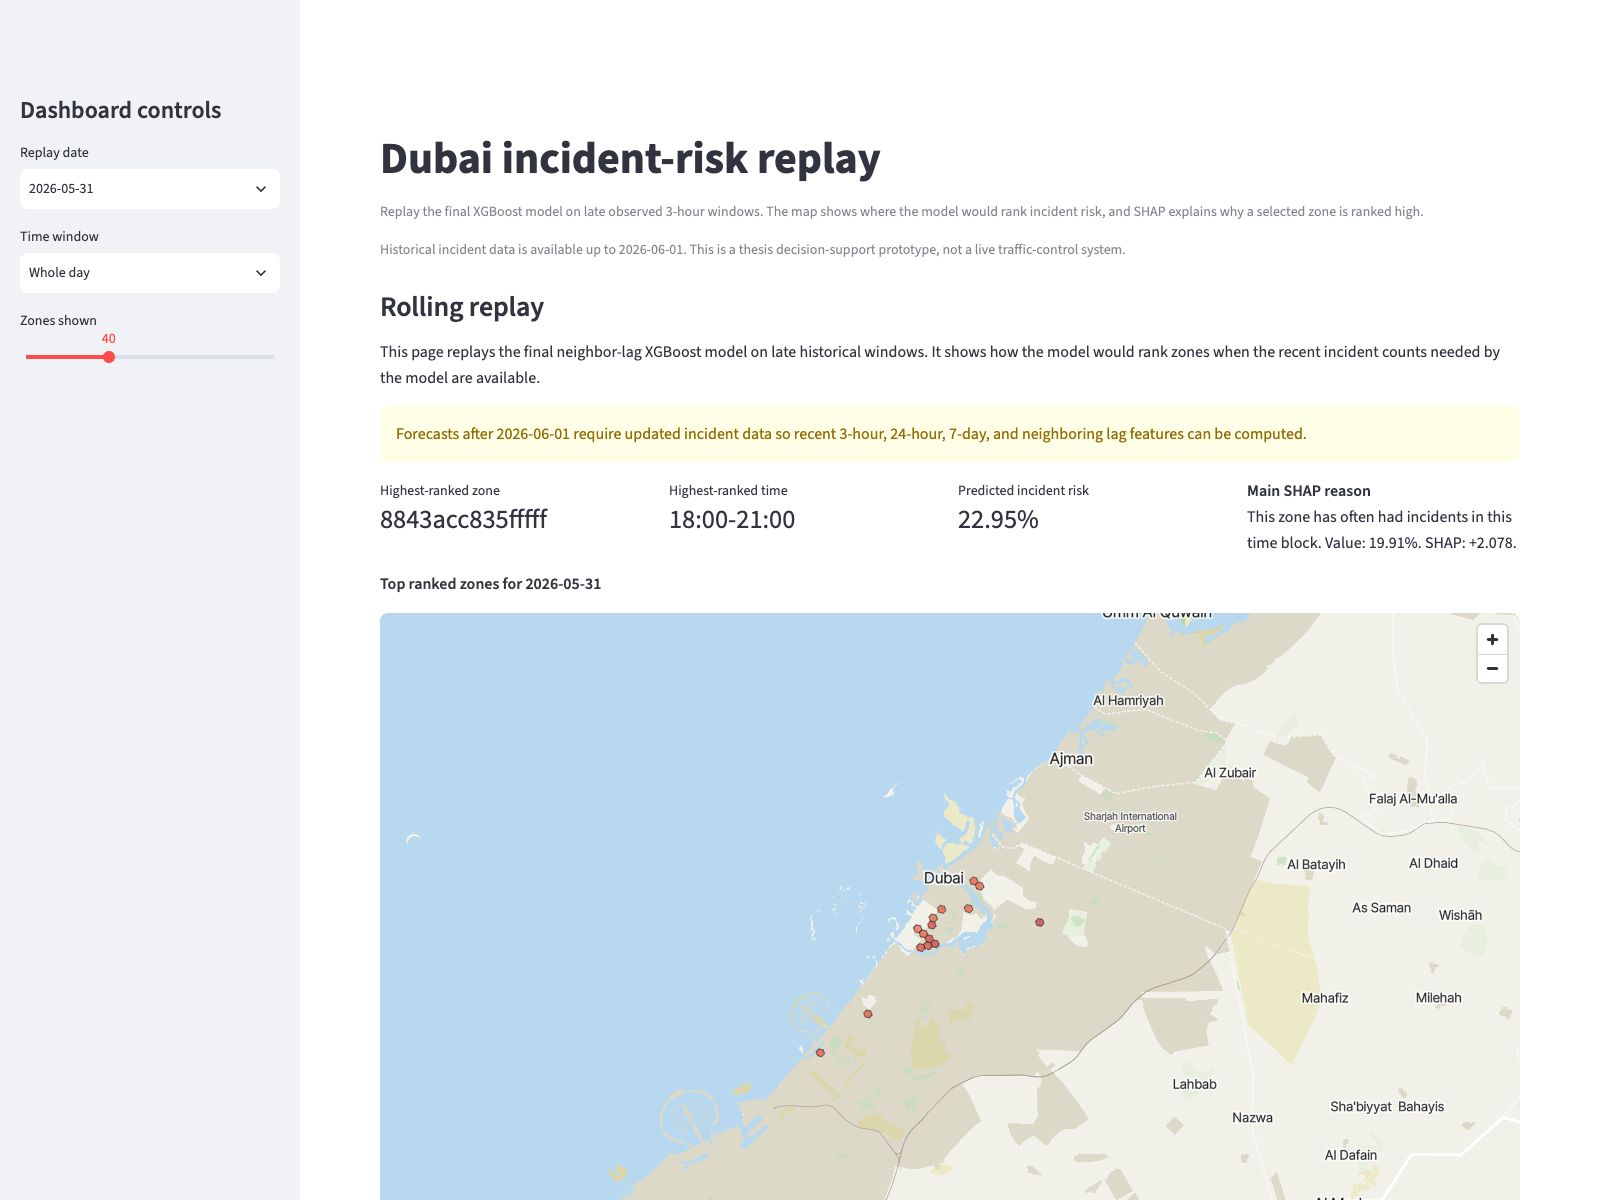
\includegraphics[width=\textwidth]{dashboard_rolling_replay.png}
    \caption{Rolling replay view with ranked H3 risk zones.}
    \label{fig:dashboard-rolling-replay}
\end{figure}

Figure~\ref{fig:dashboard-zone-explanation} shows the zone-explanation view. The selected zone has plain-language SHAP reasons, feature values, and a local contribution chart. This is the main dashboard answer to the question: why did the model rank this area and time as risky?

\begin{figure}[H]
    \centering
    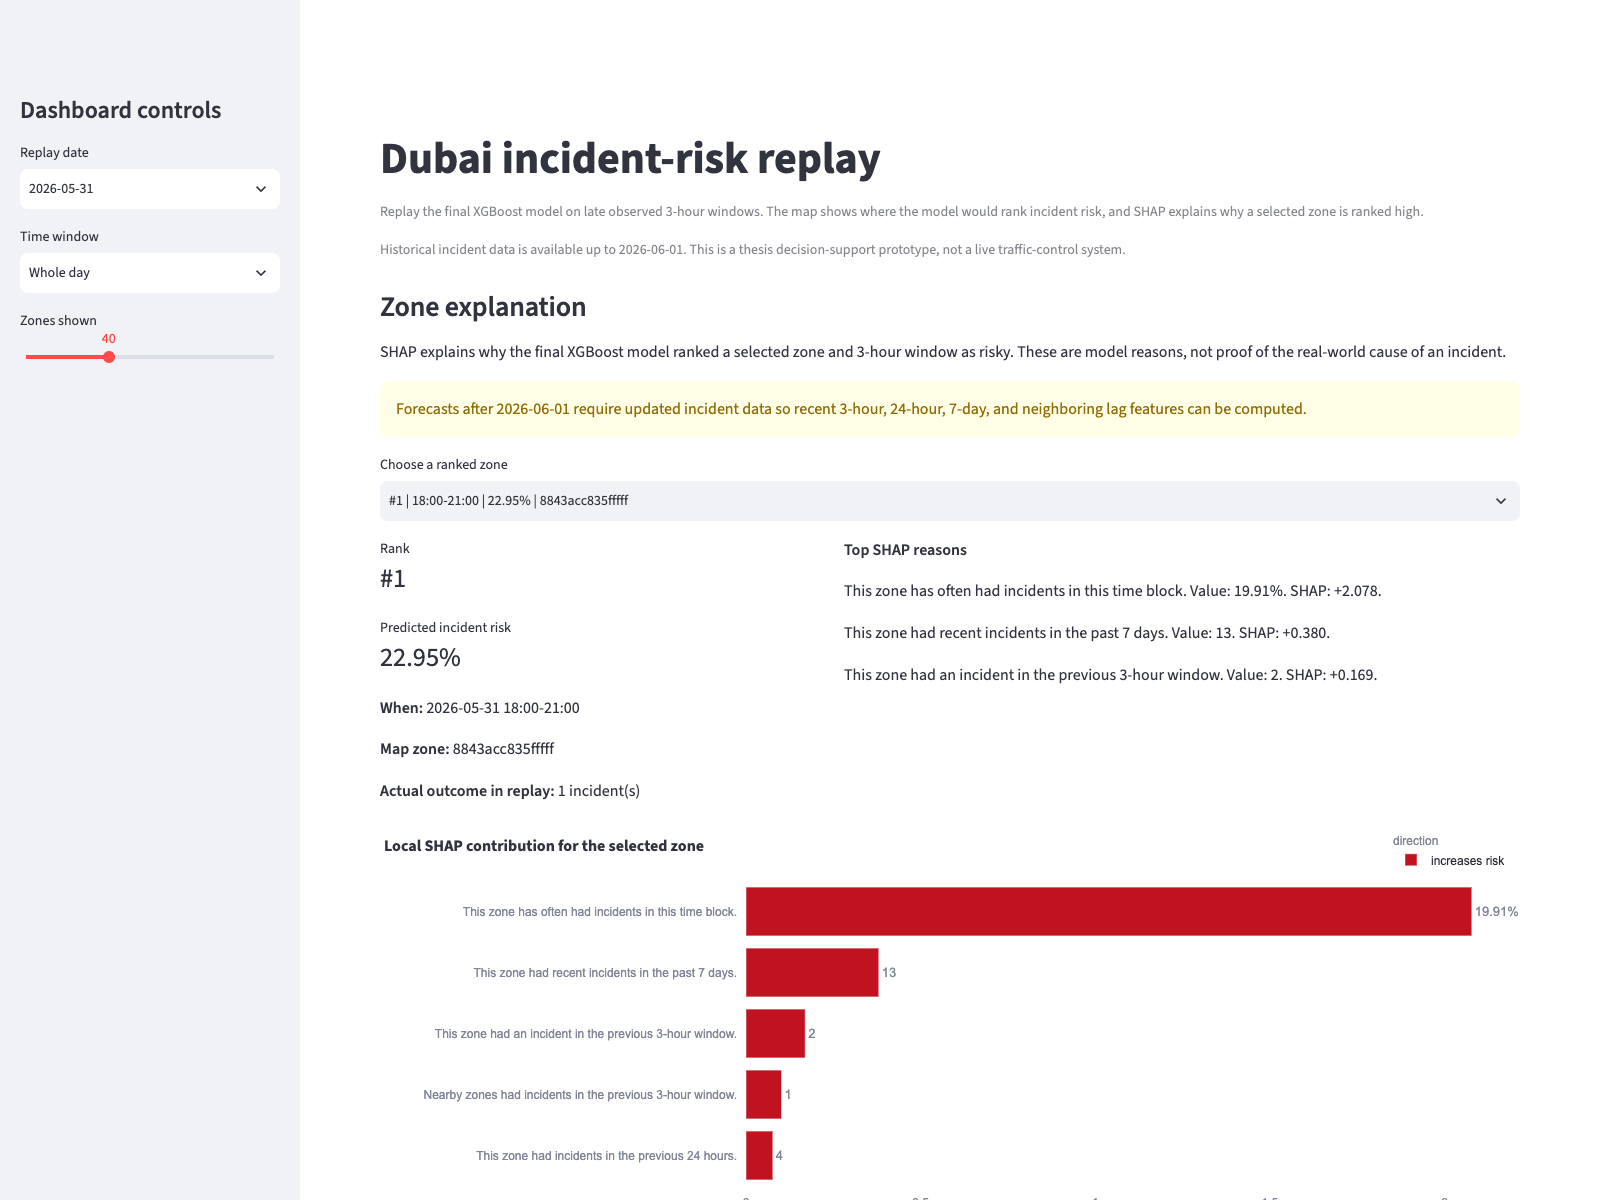
\includegraphics[width=\textwidth]{dashboard_zone_explanation.png}
    \caption{Zone-explanation view with SHAP reasons and local contribution chart.}
    \label{fig:dashboard-zone-explanation}
\end{figure}

The explanation wording is intentionally model-specific. It says that a feature increased or decreased the model's predicted risk. It does not say that the feature caused an incident. For example, a high previous 7-day incident count can be a reason for a high model score, but it is not proof that previous incidents physically caused the next one.

Figure~\ref{fig:dashboard-historical-check} shows the historical-check view. This view is kept for defense questions because it links the map output to known test-period outcomes. It helps explain the difference between a model demonstration and a claimed live forecast.

\begin{figure}[H]
    \centering
    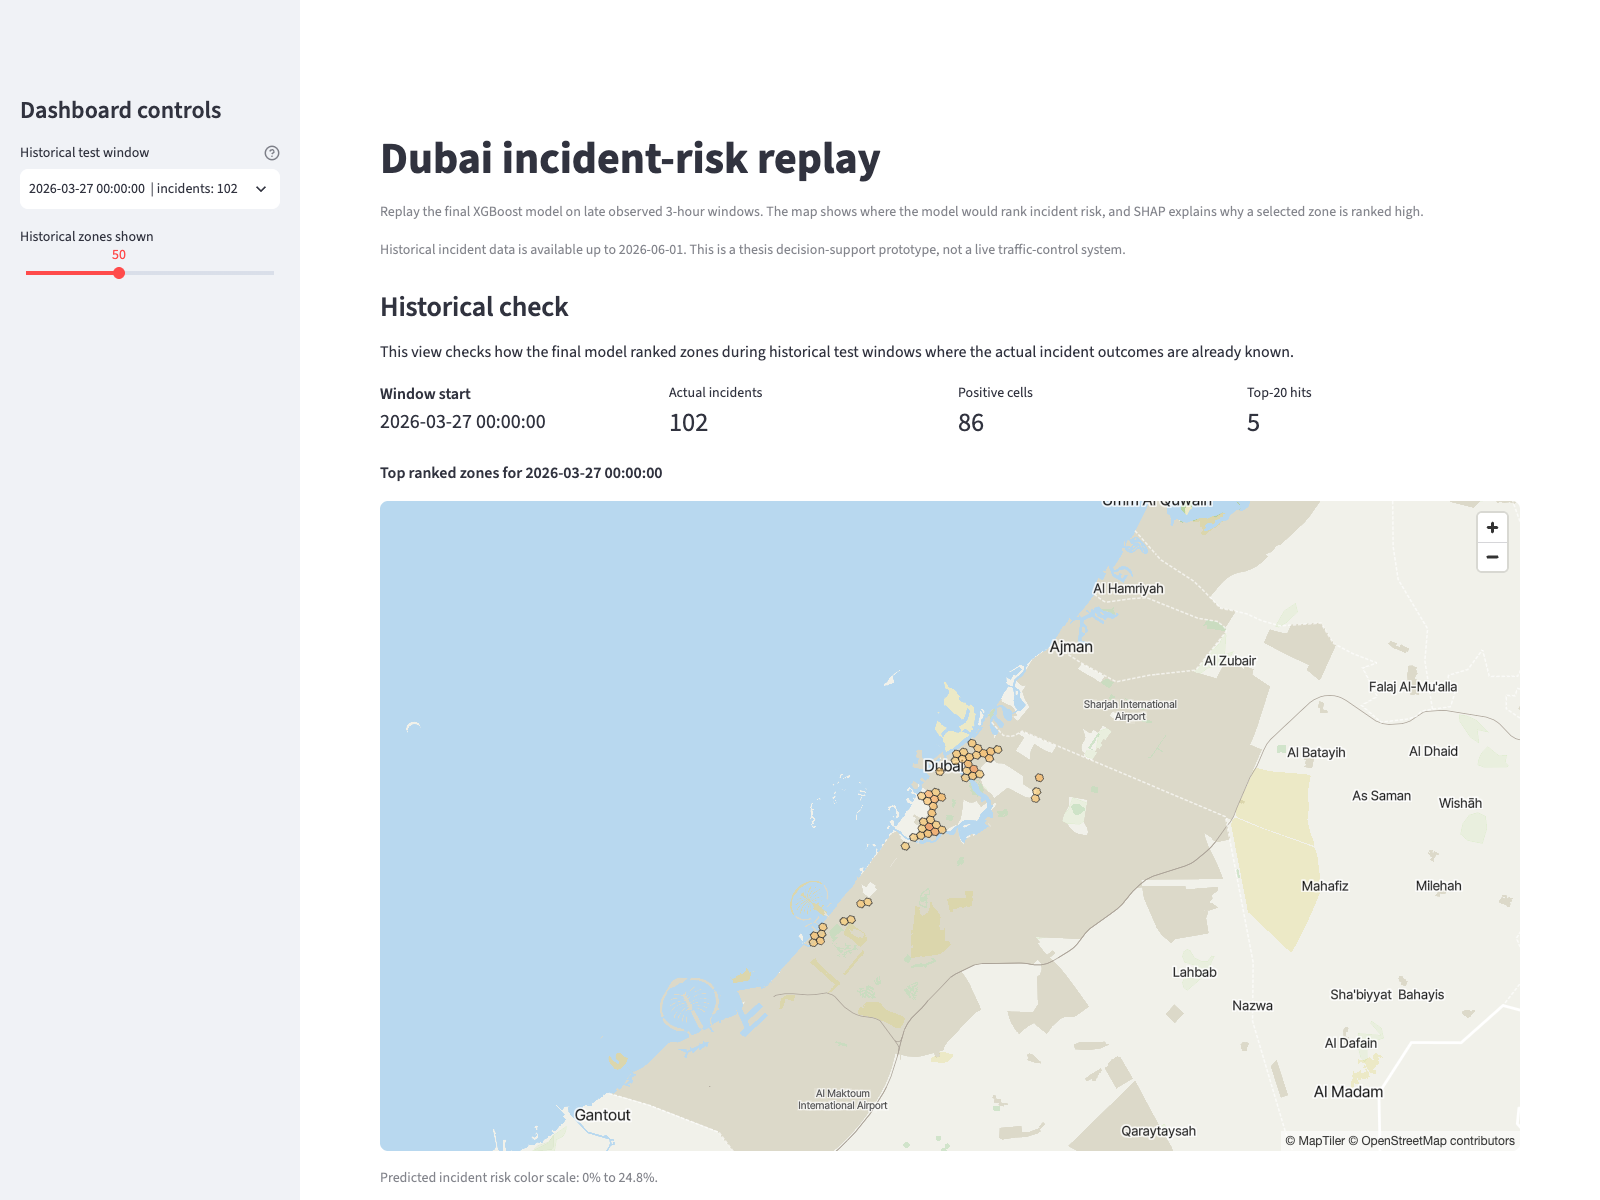
\includegraphics[width=\textwidth]{dashboard_historical_check.png}
    \caption{Historical-check view for comparing ranked H3-cell predictions with known outcomes.}
    \label{fig:dashboard-historical-check}
\end{figure}

Figure~\ref{fig:dashboard-model-evidence} shows the model-evidence view. It keeps the scientific material available without making it the first screen. This view includes the dataset scale, EDA summaries, full-grid historical evaluation metrics, hotspot ranking, and calibration reliability.

\begin{figure}[H]
    \centering
    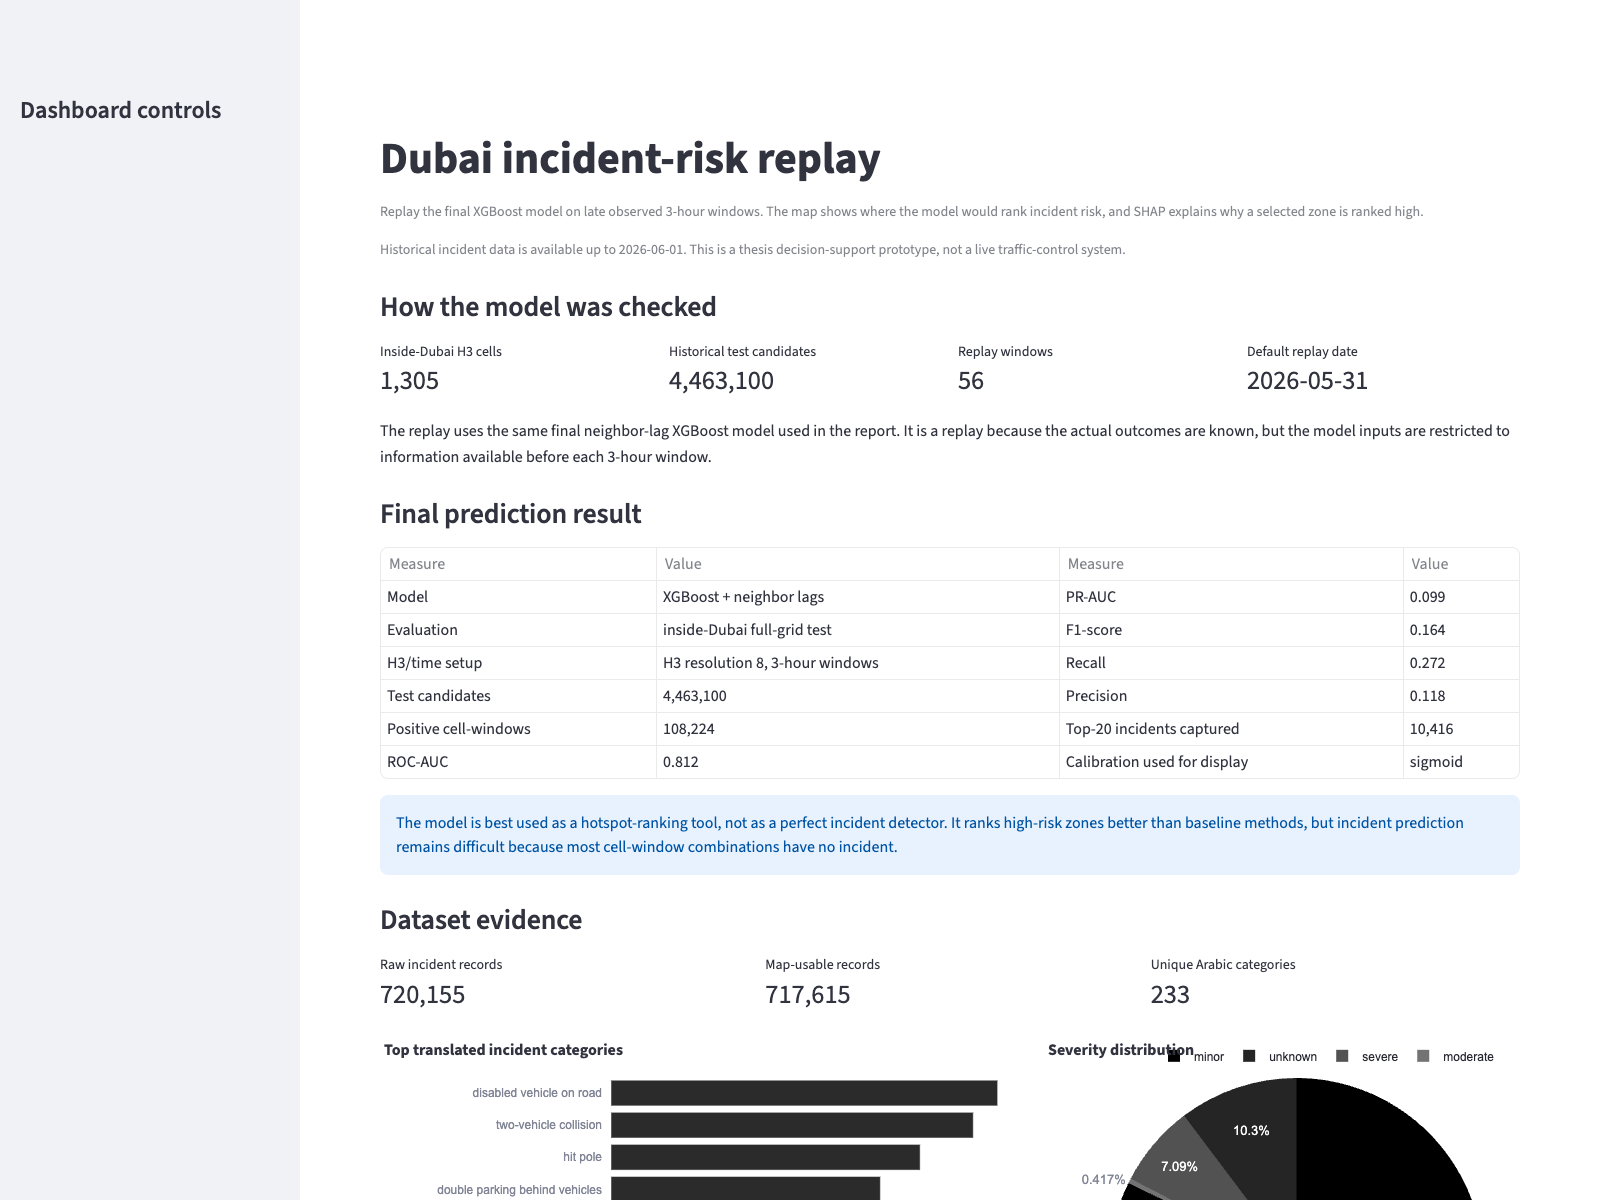
\includegraphics[width=\textwidth]{dashboard_model_evidence.png}
    \caption{Model-evidence view with EDA, full-grid metrics, hotspot ranking, and calibration reliability.}
    \label{fig:dashboard-model-evidence}
\end{figure}

\section{Use in defense}

The dashboard can be demonstrated in a short sequence. First, the rolling replay view shows where and when the final model ranks incident risk highest. Next, the zone-explanation view shows the SHAP reasons behind one selected zone. The historical-check view can then be used to show that the same grid-time formulation was evaluated against known outcomes. Finally, the model-evidence view connects the dashboard to the thesis metrics, calibration results, and EDA.

This sequence is useful for examiner questions because it separates the product story from the research evidence. The product story is where, when, and why. The research evidence is the full-grid evaluation, calibration, and explanation results. Both are needed for a final-year computer science thesis.

\section{Dashboard limitations}

The dashboard remains a prototype for inspection and communication. A real operational deployment would need live incident feeds, formal API integration, stakeholder approval, monitoring, retraining policy, and additional external features such as weather, planned events, road attributes, and traffic-flow measurements.

The current dashboard is also limited by the data cutoff. It can replay model behavior on observed windows before 1 June 2026. It cannot honestly produce rolling forecasts after that date unless consecutive updated incident records are provided. This limitation is stated in the dashboard so that the demonstration does not overclaim.

\chapter{Conclusion and future work}

This thesis built an end-to-end explainable incident-risk prediction framework for Dubai. The work began with raw Dubai Police incident records and produced a complete grid-time modeling pipeline: data audit, Arabic category translation, severity handling, coordinate correction, H3 cell assignment, 3-hour aggregation, binary target construction, chronological model evaluation, model-improvement experiments, calibration, SHAP/LIME explanation, and dashboard presentation.

\section{Completed objectives}

The first objective was to check whether the open dataset was usable for incident-risk modeling. This was achieved through the raw-data audit, checksum recording, date-range check, missing-value check, category translation map, coordinate normalization, and EDA. The audit found that the dataset is large enough for spatiotemporal modeling, with 720,155 raw records and 717,615 map-usable rows after cleaning and category filtering.

The second objective was to define a reproducible spatial and temporal formulation. This was achieved through the H3 resolution-8, 3-hour grid-time design. The final inside-Dubai evaluation grid contains 1,305 H3 cells. The target is binary: whether at least one incident occurs in a cell/window. This makes the prediction task clear and separates it from incident-duration or severity-outcome prediction.

The third objective was to compare baseline and machine-learning models. The first sampled-negative models verified that the supervised-learning pipeline worked. The stronger result used inside-Dubai full-grid validation and test scoring. In that setting, XGBoost improved over the historical-risk baseline, and ring-1 neighboring-cell lag features gave a further modest improvement.

The fourth objective was to test robustness and model choices. Historical-risk ablation showed that historical priors are important but did not reveal material training-time leakage in the expanding-history audit. H3/time-window sensitivity checks supported keeping H3 resolution 8 with 3-hour windows as the main thesis setting. The hard-negative training sample and tuned XGBoost configuration were tested but rejected because they reduced the untouched full-grid test result.

The fifth objective was explainability. SHAP was used as the main explanation method for the final XGBoost model, and LIME was used as a selected local comparison. The final SHAP results show that the model is mainly driven by historical cell-hour risk, historical cell risk, recent same-cell incident history, and neighboring-cell recent activity. The explanations are model explanations, not causal claims.

The sixth objective was a dashboard. The final dashboard presents the selected model through rolling replay on an English dashboard map. It shows ranked H3 risk zones, calibrated risk values, known replay outcomes, and SHAP reasons for selected zones. It also states that post-cutoff rolling forecasts require updated incident records because the selected model uses recent lag features.

\section{Final model choice}

The final selected model is the default XGBoost classifier with H3 resolution 8, 3-hour windows, inside-Dubai cells, historical-risk priors, same-cell lag features, and ring-1 neighboring-cell lag features. The neighboring features improve full-grid PR-AUC from 0.0967 to 0.0992 and F1-score from 0.1615 to 0.1645 compared with the same XGBoost setup without neighbor lags. At top 20 cells per test window, the final neighbor-feature model captures 10,416 incidents.

The selected model is not the most complex model tested. The hard-negative training sample reduced PR-AUC and top-k incident capture, so it was rejected. The tuned XGBoost configuration was selected using validation data but did not improve the untouched test result, so it was also rejected. The final model is therefore the simplest strong model after the completed checks, not just the last model trained.

\section{Main findings}

The first main finding is that open Dubai Police incident records can support grid-time incident-risk modeling after careful cleaning. The raw data cannot be used directly because the Arabic category field must be parsed and the coordinate order must be corrected for most valid records.

The second finding is that historical risk is a strong baseline. The model learns heavily from long-term cell/hour risk, which is expected in a spatial traffic-safety task. Machine learning improves over this baseline, but the improvement is modest rather than dramatic.

The third finding is that neighboring-cell recent activity adds useful signal. The improvement is small, but it is consistent across PR-AUC, F1, and top-k incident capture. This supports the idea that nearby H3 cells contain relevant spatial history even without a full road-network graph.

The fourth finding is that evaluation design strongly affects the reported metrics. Sampled-negative PR-AUC values are much higher than full-grid PR-AUC values because the sampled table has fewer non-incident rows. The full-grid inside-Dubai evaluation is the stronger denominator and should be treated as the main result.

The fifth finding is that calibrated risk display is necessary for the dashboard. The raw XGBoost score is useful for ranking but too confident as a probability. Sigmoid calibration reduces Brier score from 0.2127 to 0.0227 while preserving ranking metrics, making it the better dashboard-facing score.

\section{Limitations}

The work depends on a frozen open dataset ending on 1 June 2026. Forecasts after that date require updated incident records because the selected model uses recent 3-hour, 24-hour, 7-day, and neighboring-cell lag features. The dataset does not include verified traffic-flow measurements, weather, planned events, road-segment attributes, or true incident clearance time. The model therefore predicts incident occurrence risk, not duration, severity outcome, traffic delay, or signal-control action.

The coordinate correction, Arabic category translation, and H3 boundary assignment were audited, but source-data noise can still remain. The translation map should ideally be reviewed by an Arabic-speaking domain expert or the issuing entity before operational use. The Dubai boundary file may also omit some peripheral valid incident locations, which is why the final report focuses on inside-Dubai cells and keeps peripheral cells as an audit category.

SHAP and LIME explain the trained model's behaviour, not the causes of traffic incidents. The calibrated probability should be read as a model risk score tied to the training data and evaluation design, not as an official operational probability. The dashboard is a historical prototype for inspection and communication, not a deployed traffic-management system.

\section{Future work}

Future work can extend the framework in several directions. Updated incident feeds would allow rolling forecasts beyond the current cutoff and would make the dashboard closer to operational use. Weather, holidays, public events, speed limits, road attributes, and traffic-flow measurements could be added if reliable sources are available. These features may help the model distinguish recurring historical risk from current operating conditions.

Road-segment graph models could be tested after a verified Dubai road-network graph is prepared. Graph models may represent road connectivity more directly than H3 cells, but they require careful map matching and reliable road attributes. Severity-aware modeling could also be expanded beyond weighted summaries if severity labels are validated more deeply. Duration prediction would require verified clearance or resolution timestamps.

The dashboard could be extended into a controlled batch-update workflow after institutional approval. Such a workflow would need data-update checks, model monitoring, retraining policy, API design, user-access controls, and clear guidance on how risk scores should and should not be used.

Within the current thesis scope, the implemented pipeline shows that Dubai incident records can support explainable grid-time risk prediction. The strongest final claim is that the H3 resolution-8, 3-hour neighbor-feature XGBoost model gives a reproducible and interpretable baseline for ranking incident-risk zones in Dubai.


\appendix
\chapter{Literature review matrix}

This appendix provides the full citation-backed literature matrix used to support the review in Chapter 2. The main chapter keeps the synthesis compact; this appendix records the broader reviewed source base and how each source informed the thesis design.

\begingroup
\scriptsize
\setlength{\tabcolsep}{3pt}
\renewcommand{\arraystretch}{1.18}
\begin{longtable}{|p{0.8cm}|p{2.4cm}|p{3.0cm}|p{3.2cm}|p{3.9cm}|}
\caption{Literature survey for traffic incident-risk prediction and explainability}\label{tab:appendix_literature_matrix} \\
\hline
\textbf{Ref.} & \textbf{Study context} & \textbf{Target and spatial setup} & \textbf{Methods and evaluation} & \textbf{Use in this thesis} \\
\hline
\endfirsthead

\multicolumn{5}{c}{\bfseries \tablename\ \thetable{} -- continued from previous page} \\
\hline
\textbf{Ref.} & \textbf{Study context} & \textbf{Target and spatial setup} & \textbf{Methods and evaluation} & \textbf{Use in this thesis} \\
\hline
\endhead

\hline \multicolumn{5}{|r|}{Continued on next page} \\ \hline
\endfoot

\hline
\endlastfoot

\cite{aldah2010dubai} & Dubai road traffic crash thesis using crash and injury records. & Descriptive crash, casualty, and countermeasure analysis for Dubai. & Macro and micro crash analysis with injury and fatality measures. & Gives the local Dubai road-safety background and shows why Dubai needs context-specific analysis. \\ \hline
\cite{abdelfatah2015dubai} & Dubai accident trends and causes from 2003 to 2012. & City-level accident, injury, fatality, and cause trends. & Descriptive statistics and trend analysis. & Shows the limits of aggregate trend studies and supports using incident-level data. \\ \hline
\cite{abuzaid2024uae} & UAE road-user and traffic-safety variables. & Traffic-related safety/effect outcomes at UAE level. & Artificial neural network and statistical analysis. & Places AI-based traffic-safety work in the UAE context. \\ \hline
\cite{alsaleh2026dubaihotspots} & Dubai Police traffic collision records from late 2024 to mid-2025. & Temporal patterns and severity-weighted hotspots from incident points. & Temporal analysis, chi-square tests, Cramer's V, Getis-Ord Gi*, and IDW. & Confirms that Dubai Police incident records can support spatial and temporal hotspot analysis. \\ \hline
\cite{behboudi2024review} & Review of traffic accident analysis and prediction studies. & Accident occurrence, risk, severity, frequency, and duration across many settings. & Review of statistical ML, deep learning, and hybrid methods. & Positions the thesis within recent accident-prediction literature. \\ \hline
\cite{kashifi2022grid} & Chicago crashes aggregated into regular spatial grids. & Grid-time crash occurrence or risk. & Hybrid deep model with AUC-style comparisons and feature analysis. & Main support for a grid-based crash-risk formulation. \\ \hline
\cite{ren2017citywide} & Citywide accident records divided into urban regions. & Region-level accident risk over time. & Deep temporal modeling and comparisons with baselines. & Supports converting historical incidents into region/time risk labels. \\ \hline
\cite{zhou2020riskoracle} & Citywide accident forecasting with road-network and traffic features. & Fine-grained accident risk and likely subregions. & Graph neural framework, zero-risk handling, multi-task learning, and forecasting metrics. & Shows why sparsity and hotspot ranking matter in citywide risk prediction. \\ \hline
\cite{an2022hintnet} & Heterogeneous spatiotemporal accident datasets. & Accident risk or frequency across hierarchical regions. & Hierarchical knowledge-transfer network. & Supports the need to account for spatial heterogeneity between grid zones. \\ \hline
\cite{chen2024urbanrisk} & Urban accident datasets with remote sensing, POI, weather, and region features. & Urban accident risk across regions and granularities. & Multi-view graph encoding, adaptive temporal attention, and hierarchical loss. & Supports temporal, historical, and neighborhood-style features while showing richer data options. \\ \hline
\cite{saleh2022contextualvit} & Large-scale traffic accident datasets with contextual inputs. & Traffic accident risk forecasting. & Contextual Vision Transformer and baseline comparisons. & Advanced related work; contrasts with the thesis choice of simpler explainable tabular models. \\ \hline
\cite{gao2023uncertainty} & Road-level accident prediction with road-network structure. & Road-level accident frequency, severity, or risk. & Probabilistic graph neural network with uncertainty handling. & Supports future road-network extensions and uncertainty discussion. \\ \hline
\cite{kim2024sstgcn} & Seoul road-level and minute-level accident-risk dataset. & Road-level accident risk at high temporal resolution. & Sequential spatiotemporal graph convolutional network. & Shows why road-level prediction needs verified road-network data beyond the current incident snapshot. \\ \hline
\cite{ogungbire2026weather} & Weather-related crash forecasting using grid cells and external covariates. & Future crash risk or count in spatial grids. & Ensembled ConvLSTM with weather, traffic, and road data. & Supports optional weather and road-feature extension after the first incident-only model. \\ \hline
\cite{khulbe2019severe} & Accident data with spatial and temporal features. & Severe accident classification or modeling. & Machine-learning models using location and time features. & Supports the value of spatial and temporal feature engineering. \\ \hline
\cite{kalair2021duration} & Non-recurrent traffic incident duration data. & Dynamic incident-duration or hazard prediction. & Interpretable hazard-based models with Shapley-style explanations. & Clarifies that duration prediction needs clearance-time fields not yet confirmed in the Dubai data. \\ \hline
\cite{grigorev2022bilevel} & Traffic incident duration data with contextual variables. & Incident duration prediction. & Bi-level ML framework with outlier handling and feature optimization. & Supports non-recurrent incident terminology and future duration extensions. \\ \hline
\cite{grigorev2024sydney} & Sydney metropolitan traffic incident records. & Incident duration prediction and factor explanation. & XGBoost, LightGBM, and SHAP-style interpretation. & Supports tree-based incident analytics with explanation methods. \\ \hline
\cite{grigorev2022textencoding} & Incident descriptions plus traffic flow data. & Incident duration prediction. & Text encoding with ML, autoencoder, and LSTM-based components. & Supports parsing the Dubai \texttt{acci\_name} field as a useful categorical signal. \\ \hline
\cite{parsa2019realtime} & Expressway accident detection from traffic, weather, and congestion data. & Real-time accident versus non-accident detection. & LSTM, GRU, SMOTE, AUC, detection rate, and false-alarm rate. & Adjacent evidence that streaming traffic data can improve incident analytics, but outside the current open-data scope. \\ \hline
\cite{han2026secondary} & Florida freeway crash and traffic-flow data. & Secondary crash likelihood. & Hybrid ensemble and false-alarm/identification metrics. & Future-work reference for secondary incident management. \\ \hline
\cite{chen2025secondarygan} & Secondary crash data with dynamic and static variables. & Secondary crash occurrence and spatiotemporal distribution. & GAN and transformer framework for imbalance and sequence modeling. & Supports discussion of rare-event imbalance, but is too complex for the first Dubai model. \\ \hline
\cite{rifat2024explainable} & Dhaka crash database, 2017 to 2022. & Fatal versus non-fatal crash outcome. & Multiple ML models with SHAP global and local explanations. & Core example of explainable traffic-safety modeling with tree-based methods. \\ \hline
\cite{sufian2023severity} & UK road traffic accident severity data. & Accident severity prediction and analysis. & ML, econometric methods, time-series analysis, and SHAP. & Supports severity-aware secondary analysis and XAI for road safety. \\ \hline
\cite{castellani2025severity} & Crash-severity data with crash and contextual features. & Crash severity prediction. & Feature selection, AutoML-style modeling, and SHAP. & Supports transparent feature selection before final model explanation. \\ \hline
\cite{chakraborty2021severity} & Traffic crash injury severity dataset. & Injury severity classification and causal factor analysis. & Random Forest, XGBoost, DNN, and factor analysis. & Supports interpreting roadway, vehicle, and temporal factors in safety models. \\ \hline
\cite{salih2023xai} & General XAI methods review. & No traffic-specific target. & Conceptual comparison of SHAP and LIME. & Helps justify SHAP while acknowledging LIME as a comparator. \\ \hline
\cite{nobin2025starn} & FARS and ARI-BUET accident severity datasets. & Severity prediction with spatial and temporal graph attention. & STARN-GAT, macro F1, ROC-AUC, and recall. & Future-work support for graph-based severity extensions. \\ \hline
\cite{bibb2025severity} & Large accident-severity dataset and Texas subset. & Accident severity classification. & Autoencoder and dense neural network with cross-validation. & Contrasts deep severity classification with the thesis focus on explainable tabular risk models. \\ \hline
\cite{lundberg2017shap} & General model-explanation framework. & Any supervised model prediction. & Shapley additive explanations. & Main method used for global and local explanations. \\ \hline
\cite{ribeiro2016lime} & General local explanation method for black-box models. & Any black-box classifier prediction. & Comparator to SHAP for local prediction explanation. \\ \hline
\cite{chen2016xgboost} & Scalable boosted-tree learning system. & General structured supervised learning. & Regularized gradient boosting and benchmark comparisons. & Justifies XGBoost as a candidate model for the grid/time table. \\ \hline
\cite{ke2017lightgbm} & Efficient gradient-boosted decision-tree framework. & General large-scale supervised learning. & Gradient-based one-side sampling and exclusive feature bundling. & Candidate future model for large tabular incident-risk data. \\ \hline
\cite{saito2015prauc} & Imbalanced binary-classification evaluation. & General rare-positive classification. & ROC and precision-recall comparison. & Justifies PR-AUC and recall for incident-risk evaluation. \\ \hline
\cite{chawla2002smote} & General imbalanced classification. & Minority-class classification. & Synthetic minority over-sampling. & Optional imbalance reference if resampling is tested later. \\ \hline
\cite{getis1992distance} & Spatial association statistics. & Spatial clustering and hotspot detection. & Distance-based Getis-Ord statistics. & Foundation for hotspot analysis and comparison with predictive hotspots. \\ \hline
\cite{ord1995local} & Local spatial autocorrelation statistics. & Local clustering and hot/cold spot detection. & Supports severity-aware hotspot maps if included as secondary analysis. \\ \hline
\end{longtable}
\endgroup

\chapter{Model, data, and dashboard details}

This appendix records technical details that support the main chapters. The main report explains the research story; this appendix keeps the exact setup, feature list, metric definitions, and dashboard notes in one place.

\section{Data-preparation audit summary}

\begin{table}[H]
\centering
\caption{Data-preparation audit summary}
\label{tab:appendix_data_audit_summary}
\small
\begin{tabularx}{\textwidth}{L{0.36\textwidth}Y}
\toprule
\textbf{Audit item} & \textbf{Final value or decision} \\
\midrule
Raw row count & 720,155 incident-level records. \\
Raw incident period & 13 August 2018 08:17:21 to 1 June 2026 14:09:45. \\
Raw checksum & SHA-256 recorded in Chapter 3. \\
Unique raw category strings & 233. \\
Normalized category join keys & 226, because seven spacing or hyphen variants collapse during normalized joining. \\
Category exclusions & 426 rows excluded from category-level EDA because they are cancelled/admin labels or garbled source strings. \\
Category/temporal EDA rows & 719,729. \\
Valid normalized coordinates & 717,868 rows. \\
Map-usable EDA rows & 717,615 rows after category and coordinate filtering. \\
Unknown severity handling & Unknown severity is retained for incident occurrence but assigned severity weight 0 in weighted sums. \\
\bottomrule
\end{tabularx}
\end{table}

\section{Final spatial and temporal setup}

\begin{table}[H]
\centering
\caption{Final modeling setup}
\label{tab:appendix_final_setup}
\small
\begin{tabularx}{\textwidth}{L{0.34\textwidth}Y}
\toprule
\textbf{Item} & \textbf{Value} \\
\midrule
Spatial scope & Inside-Dubai H3 cells only \\
H3 resolution & 8 \\
Time window & 3 hours \\
Inside-Dubai cells & 1,305 \\
Training windows & Window index 0 to 15,955 \\
Validation windows & Window index 15,956 to 19,374 \\
Test windows & Window index 19,375 to 22,794 \\
Validation candidate rows & 4,461,795 \\
Test candidate rows & 4,463,100 \\
Test positive cell/windows & 108,224 \\
Test incidents & 115,298 \\
\bottomrule
\end{tabularx}
\end{table}

\section{Final feature list}

The final XGBoost model uses 23 input features before one-hot encoding of categorical variables.

\scriptsize
\begin{longtable}{L{0.34\textwidth}L{0.56\textwidth}}
\caption{Final neighbor-feature XGBoost inputs}
\label{tab:appendix_final_features}\\
\toprule
\textbf{Feature} & \textbf{Meaning} \\
\midrule
\endfirsthead
\toprule
\textbf{Feature} & \textbf{Meaning} \\
\midrule
\endhead
Hour block & 3-hour block of the day. \\
Day of week & Day of week for the prediction window. \\
Weekend flag & Whether the prediction window falls on a weekend. \\
Month and year & Calendar month and year. \\
Geo scope & Spatial-scope category retained for preprocessing consistency. \\
Previous 3h same-cell incidents & Same-cell incident count in the immediately previous 3-hour window. \\
Previous 24h same-cell incidents & Same-cell incident count in the previous 24 hours. \\
Previous 7d same-cell incidents & Same-cell incident count in the previous 7 days. \\
Previous 24h same-cell severity sum & Same-cell known-severity weighted sum in the previous 24 hours. \\
Previous 7d same-cell severity sum & Same-cell known-severity weighted sum in the previous 7 days. \\
Historical cell-hour risk & Train-period empirical risk for the H3 cell and hour block. \\
Historical cell risk & Train-period empirical risk for the H3 cell. \\
Historical hour risk & Train-period empirical risk for the hour block. \\
Historical global risk & Train-period global empirical risk. \\
Inside-neighbor count & Number of ring-1 H3 neighbors retained inside Dubai. \\
Previous 3h neighbor incidents & Neighboring-cell incident count in the immediately previous 3-hour window. \\
Previous 24h neighbor incidents & Neighboring-cell incident count in the previous 24 hours. \\
Previous 7d neighbor incidents & Neighboring-cell incident count in the previous 7 days. \\
Previous 24h neighbor severity sum & Neighboring-cell known-severity weighted sum in the previous 24 hours. \\
Previous 7d neighbor severity sum & Neighboring-cell known-severity weighted sum in the previous 7 days. \\
Previous 24h active-neighbor cells & Number of neighboring cells with at least one incident in the previous 24 hours. \\
Previous 7d active-neighbor cells & Number of neighboring cells with at least one incident in the previous 7 days. \\
\bottomrule
\end{longtable}
\normalsize

\section{Selected model settings}

\begin{table}[H]
\centering
\caption{Selected XGBoost configuration}
\label{tab:appendix_xgboost_settings}
\small
\begin{tabularx}{\textwidth}{L{0.34\textwidth}Y}
\toprule
\textbf{Parameter} & \textbf{Value} \\
\midrule
Model family & XGBoost binary classifier \\
Training rows used & 1,000,000 deterministic sampled rows \\
Negative sampling & Existing 5:1 sampled-negative training table, capped deterministically \\
Number of estimators & 160 \\
Maximum tree depth & 5 \\
Learning rate & 0.07 \\
Subsample & 0.85 \\
Column sample by tree & 0.90 \\
Minimum child weight & 1 \\
Tree method & Histogram-based CPU trees \\
Evaluation metric during training & Log loss \\
Class imbalance handling & \texttt{scale\_pos\_weight} computed from the training sample \\
Validation threshold & Selected on validation F1, then applied once to the test set \\
\bottomrule
\end{tabularx}
\end{table}

The tuned configuration selected by validation was not promoted because it reduced test PR-AUC, F1, and top-20 incident recall compared with the default neighbor-feature model.

\section{Metric definitions}

\begin{table}[H]
\centering
\caption{Metric definitions used in the report}
\label{tab:appendix_metric_definitions}
\small
\begin{tabularx}{\textwidth}{L{0.24\textwidth}Y}
\toprule
\textbf{Metric} & \textbf{Meaning in this thesis} \\
\midrule
ROC-AUC & Probability that the model ranks a randomly chosen positive cell/window above a randomly chosen negative cell/window, across thresholds. \\
PR-AUC & Area under the precision-recall curve. This is emphasized because positive cell/windows are rare in the full grid. \\
Precision & Share of predicted positive cell/windows that are actually positive at the selected threshold. \\
Recall & Share of actual positive cell/windows captured at the selected threshold. \\
F1-score & Harmonic mean of precision and recall at the selected threshold. \\
Brier score & Mean squared error between predicted probability and actual binary label; lower is better. \\
ECE & Expected calibration error, measuring the average gap between predicted risk and observed rate across bins. \\
Top-k recall & Share of positive cell/windows captured by the top-k ranked cells in each test window. \\
Top-k precision & Share of the top-k ranked cells that are positive, aggregated across evaluated windows. \\
Positive-window hit rate & Share of test windows with at least one positive where the top-k set captures at least one positive cell. \\
\bottomrule
\end{tabularx}
\end{table}

\section{Calibration and explanation settings}

\begin{table}[H]
\centering
\caption{Calibration and explanation settings}
\label{tab:appendix_explanation_settings}
\small
\begin{tabularx}{\textwidth}{L{0.34\textwidth}Y}
\toprule
\textbf{Item} & \textbf{Value} \\
\midrule
Calibration method selected & Sigmoid/Platt calibration \\
Calibration fitting data & Validation predictions and labels only \\
Dashboard risk value & Sigmoid-calibrated XGBoost probability \\
Raw validation threshold & 0.826884 \\
Calibrated threshold & 0.079937 \\
SHAP model explained & Final default neighbor-feature XGBoost model \\
SHAP scale & XGBoost raw-margin scale \\
SHAP background sample & 2,000 rows \\
SHAP global explanation sample & 10,000 deterministic full-grid test candidates \\
LIME background sample & 2,000 rows \\
Local explanation cases & High-risk true positive, high-risk false positive, low-score false negative, low-risk true negative \\
\bottomrule
\end{tabularx}
\end{table}

SHAP and LIME explain model behaviour. They do not establish causal effects of traffic, road, or temporal conditions.

\section{Completed experiment coverage}

\begin{table}[H]
\centering
\caption{Experiment coverage in the final report}
\label{tab:appendix_experiment_coverage}
\scriptsize
\begin{tabularx}{\textwidth}{L{0.25\textwidth}Y Y}
\toprule
\textbf{Experiment} & \textbf{Question answered} & \textbf{Final decision} \\
\midrule
Sampled-negative baseline & Does the end-to-end supervised pipeline train and score models correctly? & Kept as a pipeline check. \\
Inside-Dubai full-grid evaluation & How do models perform on the true inside-Dubai validation/test denominator? & Used as the main model-selection basis. \\
Historical-risk audit & Are historical features useful, and do they create material training-time leakage? & Historical priors retained; expanding-history result was stable. \\
H3/time sensitivity & Is the H3-8, 3-hour setting defensible? & H3-8 and 3-hour windows retained as the best balance. \\
Neighbor-lag features & Does adjacent-cell recent history improve the model? & Promoted into the final model path. \\
Hard-negative training & Does a 70/30 hard-negative sample improve the final model? & Rejected because full-grid PR-AUC and top-k capture fell. \\
XGBoost tuning & Does validation-selected tuning improve the untouched test result? & Rejected because the default neighbor-feature model remained stronger. \\
Calibration & Can risk scores be made more reliable for dashboard display? & Sigmoid calibration promoted for dashboard risk values. \\
SHAP/LIME & Can the selected model be explained globally and locally? & SHAP retained as main explanation method; LIME retained as supporting local check. \\
Dashboard & Can the result be inspected as where, when, and why? & Implemented as rolling replay with an English dashboard map and SHAP reasons. \\
\bottomrule
\end{tabularx}
\end{table}

\section{Dashboard reproducibility notes}

\begin{table}[H]
\centering
\caption{Dashboard implementation summary}
\label{tab:appendix_dashboard_summary}
\small
\begin{tabularx}{\textwidth}{L{0.32\textwidth}Y}
\toprule
\textbf{Item} & \textbf{Dashboard setting} \\
\midrule
Application stack & Streamlit for the app shell, PyDeck for MapTiler risk maps, and Plotly for charts. \\
Main view & Rolling replay on complete observed days before the 1 June 2026 data cutoff. \\
Map layer & H3 resolution-8 polygons over a MapTiler English-language map. \\
Displayed risk value & Sigmoid-calibrated XGBoost probability. \\
Explanation method in dashboard & SHAP top reasons and local contribution chart. \\
Runtime data design & Compact precomputed dashboard files; the app does not load the raw 720,155-row file or the full 4.46 million-row test matrix during interaction. \\
Forecast limitation & Dates after the cutoff require updated incident records so recent same-cell and neighboring lag features can be recomputed. \\
\bottomrule
\end{tabularx}
\end{table}

\chapter{Research paper draft attachment}

\begin{center}
\Large\textbf{Explainable grid-time traffic incident risk prediction in Dubai}\\[0.4cm]
\normalsize Sparsh Aggarwal\\
Department of Computer Science, BITS Pilani Dubai Campus
\end{center}

\section*{Abstract}

This paper presents an explainable machine-learning framework for non-recurrent traffic incident risk prediction in Dubai. The work uses 720,155 Dubai Police incident records from 13 August 2018 to 1 June 2026. Arabic category labels are translated and parsed, coordinates are normalized, and incidents are mapped to H3 cells and 3-hour time windows. The prediction target is binary: whether a cell/window contains at least one incident. Models are trained chronologically and evaluated on a full inside-Dubai grid. The selected model is an XGBoost classifier with historical-risk, same-cell lag, and ring-1 neighboring-cell lag features. Neighboring-cell features improve full-grid PR-AUC from 0.0967 to 0.0992 and F1-score from 0.1615 to 0.1645 compared with the same XGBoost setup without neighbor features. Sigmoid calibration improves dashboard probability reliability, and SHAP explanations identify historical cell-hour risk, same-cell recent incidents, and neighboring recent incidents as the main model drivers. The final dashboard demonstrates rolling replay on an English dashboard map with zone-level SHAP reasons.

\section*{Keywords}

Traffic incident prediction; explainable AI; H3 grid; XGBoost; SHAP; Dubai; road safety.

\section{Introduction}

Non-recurrent traffic incidents such as crashes, vehicle breakdowns, obstructions, and stalled vehicles create irregular disruptions in urban road networks. Dubai has been studied in earlier road-safety work, including crash-cause and trend analysis \cite{aldah2010dubai,abdelfatah2015dubai}. Recent Dubai hotspot work shows that Dubai Police records can support spatial and temporal collision analysis \cite{alsaleh2026dubaihotspots}. The remaining gap is an explainable prediction framework that converts incident records into a grid/time model and explains high-risk outputs.

The contribution of this paper is a reproducible incident-only framework for Dubai. It uses H3 cells as spatial units, 3-hour windows as temporal units, chronological evaluation, full-grid test scoring, calibrated XGBoost risk scores, and SHAP explanations. The work is designed as a historical decision-support prototype, not a live deployment.

\section{Related work}

Traffic accident prediction has moved from aggregate descriptive studies toward spatiotemporal modeling. Citywide risk models show that historical incident patterns can be converted into region/time risk estimates \cite{ren2017citywide,zhou2020riskoracle}. Grid-based crash-prediction work supports aggregating point crashes into spatial cells before prediction \cite{kashifi2022grid}. Recent urban accident-risk studies also show that spatial proximity, regionality, and sparsity affect predictive performance \cite{chen2024urbanrisk}.

Explainable traffic-safety models have mainly focused on fatality, severity, or duration prediction. SHAP has been used to explain traffic fatality and severity models \cite{rifat2024explainable,sufian2023severity}. LIME provides a model-agnostic local explanation alternative \cite{ribeiro2016lime}. This paper applies these ideas to a different target: whether a Dubai H3 cell contains at least one reported non-recurrent incident in a 3-hour window.

\section{Data and preprocessing}

The source data is an open Dubai Police traffic incident dataset from Dubai's Data and Statistics portal. The frozen snapshot contains 720,155 rows and six raw fields: incident ID, occurrence time, Arabic category, two coordinate fields, and load timestamp. The date range is 13 August 2018 08:17:21 to 1 June 2026 14:09:45.

The Arabic category field contains 233 unique values. These values are translated and parsed once, then joined back to the full dataset. Unknown severity is retained as a separate class and assigned severity weight 0 for weighted sums. Unknown-severity incidents remain in the binary incident-occurrence target because they are real incident records.

Coordinate validation showed that most valid source records used reversed coordinate order. The cleaning process keeps the raw coordinate fields and adds normalized longitude, latitude, and coordinate-status fields. After category and coordinate filters, 717,615 rows are usable for map-based EDA.

\section{Method}

Each incident is assigned to an H3 resolution-8 cell and a 3-hour window. For each inside-Dubai H3 cell and each time window, the target is 1 if at least one incident occurs and 0 otherwise. The final inside-Dubai grid contains 1,305 cells. The test period contains 4,463,100 candidate cell/windows and 108,224 positive cell/windows.

The final feature set includes calendar variables, same-cell lag features over 3 hours, 24 hours, and 7 days, train-period historical-risk priors, and ring-1 neighboring-cell lag features. Neighboring-cell features are computed from H3 ring-1 cells inside Dubai only. All lag features use windows before the target window.

Historical risk, Logistic Regression, Random Forest, and XGBoost are evaluated. The selected model is the default XGBoost classifier with the neighbor-lag feature set. SHAP explains global and local model behaviour \cite{lundberg2017shap}. LIME is used as a local model-agnostic comparison on selected cases \cite{ribeiro2016lime}.

The evaluation is chronological. Early windows are used for training, the next block of windows is used for validation and calibration, and the final block is used for test reporting. The test set is a full inside-Dubai grid, not a sampled-negative table. This matters because incident-positive cell/windows are rare. PR-AUC and top-k hotspot metrics are therefore reported along with ROC-AUC, recall, and F1-score.

\section{Results}

The first full-grid comparison shows that XGBoost improves over historical risk. Historical risk obtains PR-AUC 0.0882 and F1-score 0.1522. XGBoost with the initial feature set obtains PR-AUC 0.0967 and F1-score 0.1615. Adding ring-1 neighboring-cell lag features improves XGBoost to PR-AUC 0.0992, ROC-AUC 0.8120, recall 0.2720, and F1-score 0.1645.

\begin{table}[H]
\centering
\caption{Paper draft summary of final full-grid result}
\label{tab:paper_final_result}
\small
\begin{tabular}{lrrrr}
\toprule
\textbf{Model} & \textbf{ROC-AUC} & \textbf{PR-AUC} & \textbf{Recall} & \textbf{F1} \\
\midrule
Historical risk & 0.7990 & 0.0882 & 0.2679 & 0.1522 \\
XGBoost without neighbor lags & 0.8067 & 0.0967 & 0.2630 & 0.1615 \\
XGBoost with neighbor lags & 0.8120 & 0.0992 & 0.2720 & 0.1645 \\
\bottomrule
\end{tabular}
\end{table}

At top 20 cells per test window, the final neighbor-feature XGBoost model captures 9,138 positive cell/windows and 10,416 incidents. This supports its use as a hotspot-ranking model. A hard-negative sample and a tuned XGBoost configuration were also tested, but both reduced the untouched full-grid test result. Sigmoid calibration reduces Brier score from 0.2127 to 0.0227 while preserving PR-AUC and top-k ranking.

SHAP identifies historical cell-hour risk as the strongest feature group, followed by year, historical cell risk, previous 7-day same-cell incident count, and previous 7-day neighboring-cell incident count. LIME broadly agrees with SHAP on selected local cases. The explanations indicate that the model mainly learns long-term zone/time risk and recent local or nearby activity. These are model explanations, not causal claims.

\section{Discussion}

The strongest result is not that the model predicts every incident. It does not. The useful result is that the model gives a reproducible way to rank zones by incident risk and explain the ranking. Historical risk is already a strong baseline, so the machine-learning improvement is modest. The neighboring-cell feature experiment shows that nearby recent activity adds signal, but the final model is still mainly driven by long-term cell/hour risk.

The failed experiments are also informative. The tested hard-negative sample reduced full-grid PR-AUC and top-k incident capture, so it was not promoted. The tuned XGBoost candidate was selected using validation data but did not improve the untouched test period, so the default neighbor-feature model was retained. This gives a clearer final model-selection story than simply reporting the last model trained.

\section{Dashboard demonstration}

The dashboard presents the final model as a rolling replay. It defaults to the latest complete observed day before the data cutoff and shows top-ranked H3 zones on an English dashboard map. A separate zone-explanation view shows the top SHAP reasons, feature values, and contribution bars for a selected zone. The dashboard states that forecasts after 1 June 2026 require updated incident records because the final model uses recent lag features.

\section{Conclusion}

The study shows that open Dubai Police incident records can support explainable grid-time incident-risk prediction after careful cleaning, coordinate correction, and target construction. The final model does not solve live traffic management, but it provides a reproducible and interpretable baseline for ranking incident-risk zones in Dubai. Future work should add updated incident feeds, weather, road attributes, traffic-flow measurements, and road-network graph features if those data sources become available.


\bibliographystyle{ieeetr}
\bibliography{../../references}

\chapter*{List of publications or conference presentations}
\addcontentsline{toc}{chapter}{List of publications or conference presentations}
No external publication or conference presentation has been completed at the time of this report. A research-paper draft based on the thesis work is attached in Appendix C for the course submission requirement.

\end{document}
